\documentclass{gdutarticle}
%\usepackage[backend=biber,style=gb7714-2015]{biblatex}
%\addbibresource{References.bib}

\infosetup{
  subject = 本科毕业设计(论文),
  title  = 基于TUSS4470芯片的超声波接近传感器设计,
%   subtitle = Design of calculation and analysis system for automobile power economic performance
  college = 机电工程学院,
  major   = 机械电子工程,
  grade   = 2019级(2)班,
  stuid   = 3119000323,
  name    = 周浩能,
  teacher = 刘桂贤
}



\includeonly{
	chapter/ZhAbstract.tex,
	chapter/EnAbstract.tex,
	chapter/第一章.tex,
	chapter/第二章.tex,
	chapter/第三章.tex,
	chapter/第四章.tex,
	chapter/第五章.tex,
	chapter/第六章.tex,
	chapter/conclusion.tex,
	chapter/introduction.tex,
	chapter/analyze1.tex,
	chapter/analyze2.tex,
	chapter/thank.tex,
	chapter/appendix1.tex,
	chapter/appendix2.tex
}




\begin{document}

%!TEX root = ../main.tex
\begin{ZhAbstract}
    在自动化生产中,到位传感器的稳定性和精度有着十分重要的作用,本毕业设计拟基于TUSS4470集成芯片开发设计超声波接近传感器,主要用于钢化玻璃自动化生产线到位检测。相比传统的单片机控制,本设计采用CPLD芯片来产生传感器驱动控制信号,获得了比传统型控制信号精度更高、稳定性更好的驱动信号。\par
    传感器硬件设计包括了CPLD最小系统设计、TUSS4470芯片外围电路设计以及PCB设计,软件设计包括了芯片配置、脉冲产生、到位检测等部分。本设计采用多次发送脉冲波,设定检测阈值判断检测状态的检测策略,可以根据应用场景调整脉冲波发射的次数以及脉冲数,极大提高了传感器在生产应用中的灵活性和可靠性。\par
    实验表明:该传感器可以检测$100mm\sim200mm$范围内的物体,检测精度可达到$1mm$,检测周期为$10ms$。本设计已达到预期目的,具有稳定性好、精度高、适用场景丰富等特点。
    
    \ChineseKeyWord 超声波接近传感器、CPLD芯片、TUSS4470集成芯片、检测策略
    
\end{ZhAbstract}
%!TEX root = ../main.tex
\begin{EnAbstract}
    
    This design aims to solve the problem of detecting the positioning of tempered glass on the production line. A highly stable, flexible and widely applicable ultrasonic proximity sensor is developed. Compared with traditional single-chip control, this design uses a CPLD chip to generate sensor driving control signals. Combined with the TUSS4470 integrated chip, higher precision and more stable driving signals can be obtained. At the same time, the design uses a detection strategy of multiple pulse waves and a set detection threshold to judge the detection status. By adjusting the number of pulse wave emissions and the number of pulses, the flexibility and reliability of the sensor in production applications are improved.
    
    The design aims to create an ultrasonic proximity sensor capable of detecting objects within the range of $100mm \sim 200mm$ with a detection accuracy of $1mm$.
    
    This article will detail the design process and working principle of the ultrasonic proximity sensor's hardware and software components. After completing the simulation of the hardware and software components, physical welding and production will be performed, and the program will be debugged using an oscilloscope. Finally, an experimental plan will be designed to test the sensor's performance parameters and echo characteristics.
  
  
    \EnglishKeyWord ultrasonic proximity sensor, CPLD chip, TUSS4470 integrated chip , detection strategy
\end{EnAbstract}

\makecontent
	%------------------第一章---------------------------
	\newpage
	\section{绪论}
    \subsection{超声波接近传感器的研究背景和意义}
    \subsubsection{超声波接近传感器的发展}
    超声波接近传感器是一种常用的非接触式测距传感器,它能够将物体到传感器的距离转化为电信号,实现物体的远近判断。超声波接近传感器广泛应用于工业自动化、机器人、无人驾驶等领域。随着技术的发展,超声波接近传感器的性能不断得到提高。    
    超声波接近传感器的发展经历了三个阶段。第一代超声波接近传感器采用固定式超声波传感器,能够实现对物体距离的测量,但是存在精度不高、抗干扰能力弱等问题。第二代超声波接近传感器采用微机处理技术和数字滤波技术,在一定程度上提高了抗干扰能力。第三代采用了新型材料和新技术,如MEMS技术、FPGA技术等,进一步提高了系统的测量精度、稳定性。
    \subsubsection{超声波接近传感器国内外研究现状}
    \paragraph{国内研究现状}
	国内研究人员在超声波接近传感器方面取得了突破性进展,主要集中在回波信号检测、超声换能器研发、超声发射脉冲选取等方面。
	
	在超声波换能器设计方面,2004年,通过对Vmos场效应管开关元件发射电路进行分析,矿业研究所的马庆云等研究发现,触发脉冲对超声波换能器的发射功率产生影响,最大发射功率对应的触发脉冲宽度是其谐振周期的$\frac{1}{2}$\upcite{超声波测距传感器的研究6}。这一发现对新型超声波换能器发射电路的研究具有指导作用,因为它可以克服传统调频超声波系统必须使用宽带超声传感器的问题,通过调整触发脉冲宽度来控制发射功率,从而实现对超声波发射信号的精确控制。
	
	2005年,李希胜等人在北京科技大学进行了一项研究,即窄带调频超声波距离检测。该技术不仅能够以极低的瞬时超声波功率实现极高的平均发射功率,而且还可以通过普通的超声波传感器实现,大大降低了传感器的成本。
	
	2006年,潘仲明开展了大作用距离超声波传感技术的研究。该研究在谐振频率为24.5$kHz$基础上,研发出一种新型超声波传感器,其作用距离可以达到$31m$以上,测量误差低于$3\%$\upcite{超声波测距传感器的研究7}。
		
	在超声波发射脉冲选取方面,程晓畅在2006年提出了一种基于雷达信号处理中的脉冲压缩技术的超声波发射脉冲选取方法,使用伪随机二进制序列来提供超声波发射的压缩信号,获得更高的信号功率和更小的脉冲宽度,从而提高了超声波信号的分辨率和检测精度\upcite{超声波测距传感器的研究8}。这种方法有效地解决了传统超声波检测中信号功率不足、信号宽度大等问题,为超声波检测技术的提高提供了重要的理论基础和实验支持。
	
	2008年,在嵌入式应用中,杜晓同时考虑到测距量程和精度,利用$40kHz$与$20kHz$两种频率的超声波进行测距,将脉冲压缩技术很好的与双频超声测距技术超声波测距中相融合,使超声波接近传感器即可以增加检测范围,又可以得到更高的检测精度\upcite{超声波测距传感器的研究9}。
		
	2007年,在仪表技术中,陈平等人将超声波检测技术与测距算法相互融合,设计了一种液位监控传感器。该超声波传感器利用了温度传感器对声速进行温度补偿,从而提高了检测分辨率。
	
	在移动机器人视觉方面的研究中,田志宏在2007年设计了一种智能避障的自动轮椅车,并在传感器技术学报上发表了相关成果\upcite{超声波测距传感器的研究10}。王洪青研究出了一种并行超声波测距系统,在轮椅车上的各个方向安装了多组传感器,实现多传感器数据融合,实时检测距离的效果。
	
    \paragraph{国外研究现状}
	同样,超声波接近传感器在国外也有了很大的发展。
	
	2013年2月,在伦敦帝国大学,Joseph Jackson,Rahul Summa等采用渡越时间法来进行超声波测距,作者将该方法应用于移动机器人、物体结构探测和医学成像领域的研究\upcite{超声波测距传感器的研究11}。
	
	2010年12月,里斯本大学的研究人员Ricard Queiros和Francisc Corre Alegria提出了一种新型的超声波接近传感器测距方法。该方法利用了交叉相关联和正弦发生器技术,提高了在空气中测距的分辨率。交叉相关技术通过将发送信号与接收信号相融合,检测超声波在空气中传播的时间,从而精确测量距离;正弦发生器则可以检测超声波传播过程中的相移,进而提高测距的分辨率。
	
	2011年,JiDe Huang和Chih Kung Lee在康奈尔大学提出了一种新的高精度超声波测距系统,该系统采用基于峰值检测和干涉技术的方法。该超声波测距系统的特点是通过硬件设计提高了测距系统的精度,而不依赖于复杂的算法,在不增加成本的情况下提高了传感器的精度\upcite{超声波测距传感器的研究14}。
	
    
    \subsubsection{超声波接近传感器的研究意义}
    TUSS4470芯片作为一种新型的超声波传感器芯片,具有高精度、低功耗和多种工作模式等特点,可以满足现代工业和自动化控制对于测量、检测、控制和导航等方面的需求。因此,基于TUSS4470芯片的超声波接近传感器的研究成为了一个热门话题,其可以应用于智能家居、无人机、自动驾驶车辆、机器人等领域,具有广阔的应用前景和市场前景。\par
    此外,在传统的超声波驱动控制电路中,一般是采用模拟电路或者单片机来控制。由模拟电路驱动的超声波传感器抗干扰性差,而由单片机驱动的超声波传感器,由于其使用外部中断触发的机制,导致无法精确控制时序逻辑,从而难以达到与超声探头匹配的驱动频率,而超声波传感器的检测精度直接取决于其发出脉冲宽度的精度\upcite{CPLD在超声波传感器驱动控制电路中},当脉冲宽度无法匹配时将使得传感器的精度降低,因此使用CPLD芯片控制产生精确的脉冲宽度对提高传感器的检测精度有着十分重要的意义。\par
    本设计采用型号为EPM240T100C5N的MAX II系列芯片,它是一种高集成度、电可擦除、CMOS宏阵列可编程逻辑器件\upcite{基于STM32和超声波测距的倒车雷达预警系统设计},可以产生ns级别的控制信号\upcite{CPLD芯片介绍},配合TUSS4470超声驱动芯片,可精确控制发送脉冲的次数、频率以及脉冲宽度。同时,CPLD芯片编程采用时序逻辑,发送、接收、检测脉冲信号的时间可进行精确控制,这让超声检测策略可以变得更加丰富合理。
    \subsection{超声波接近传感器的原理}
    \subsubsection{超声波介绍}
      超声波是一种弹性机械波,可以在气体、液体和固体中传播。人们可以听到的声音频率范围是$20Hz\sim20kHz$,超出该范围的声音被称为低频声波或超声波。超声波在相同的传播介质里的传播速度相同,在大气条件下的传播速度约为$340m/s$,相对于电磁波的传播速度$3\times10^8m/s$来说非常慢。超声波的纵向分辨率较高,对许多干扰因素如光线、电磁波都不敏感,受环境因素的影响较小,且超声波在遇到物体反射时,入射角和反射角近似相等,方便用于测量较近目标的距离\upcite{车载可视倒车雷达预警系统的研制}。
      
      超声波的传播方向与振动方向一致,是纵向振动的弹性机械波,其波动方程描述方法与电磁波相似,如式\ref{波动方程}所示。
    \begin{equation}
    	A=A(x)cos(\omega t+kx)
    	\label{波动方程}
    \end{equation}
	式中\quad$x$---传播距离;\par
	\quad$\omega$---频率
	\begin{equation}
		A(x)=A_0 e^{-\alpha x}
		\label{振幅方程}
	\end{equation}
	式中\quad$A(x)$---振幅;\par
		\quad$\alpha$---衰减指数
	\begin{equation}
		\alpha=a f^2
		\label{衰减指数}
	\end{equation}
	式中\quad $a$---介质常数;\par
	   \quad $f$---振动频率\par
    根据式\ref{衰减指数}我们可以得出,当频率越高时,振幅衰减程度越大,传播的距离也就越短。这是因为声波在空气介质里传播时,会与空气分子间存在运动摩擦,导致能量被吸收损耗。但超声波频率越高时,其指向性就越强,有利于回波的反射和检测。权衡指向性和距离损耗两点因素,为达到良好的测距效果,在设计超声波接近传感器时,我们选用中心频率为$f=30kHz$的超声波换能器。
    \subsubsection{超声换能器的结构}
    超声换能器是一种将其它形式的能转换为超声能或是将超声能转换为其他形式的能的装置。在实际应用中,常用的超声换能器主要包括电声型和流体动力型两类\upcite{面向机器人安全避障的MEMS压电超声接近觉传感器的研究39}。
    电声型超声换能器主要包括压电换能器、磁质伸缩换能器和静电换能器三种。其中,压电换能器是最常用的一种,它利用压电效应将电能转化为机械能或将机械能转化为电能\upcite{车载可视倒车雷达预警系统的研制}。磁质伸缩换能器则是利用磁性材料的磁致伸缩效应实现能量转换,静电换能器则是利用静电场的作用实现能量转换。
    流体动力型超声换能器主要包括气体和液体两种类型。其中,气体型是利用气体流动产生的声波进行能量转换,液体型则是利用液体流动产生的声波进行能量转换。这两种传感器在实际应用中具有一定的局限性,主要是在响应频率、灵敏度、稳定性等方面存在一定的问题。
    超声换能器的结构形式是多种多样的,不同的超声换能器名称也不尽相同。在超声检测和诊断中,人们通常将超声传感器称作探头。在工业领域中,采用流体动力型传感器的常常被称为“哨”或“笛”,其结构形式也各异\upcite{车载可视倒车雷达预警系统的研制13}。\par
    压电式超声波换能器是一种电声型传感装置,它利用压电材料的特性将电能转换为机械振动,将机械振动转换为电能。压电式超声波换能器主要由压电晶片、楔块、接头等组成,是超声检测中最常用的一种传感装置,是超声波检测装置的重要组成部分。在医学影像诊断、非破坏性检测、声纳定位等领域中得到广泛应用。\par
    超声波换能器的核心是压电晶片,它可以产生逆压电效应和正压电效应。当压电晶片接收到发射电脉冲时,逆压电效应会使晶片振动并发射超声波;而当晶片接收到超声波时,正压电效应会使晶片发生机械变形,并将其转换成相应的电信号。通常采用双压电陶瓷晶片制成超声波换能器,其中一个晶片用于发射超声波,另一个用于接收超声波\upcite{车载可视倒车雷达预警系统的研制15}。
    \begin{figure}[!h]

    	\begin{minipage}{0.5\textwidth}
    		\centering
    		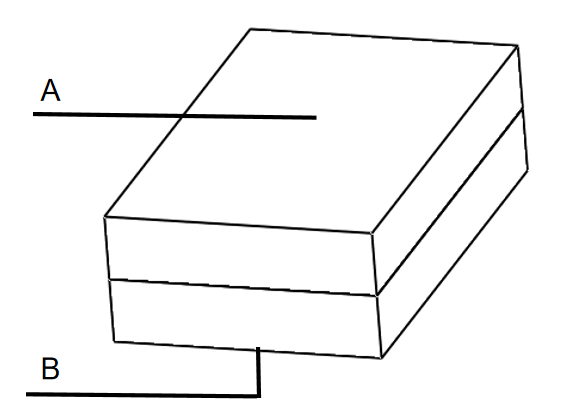
\includegraphics[height=4cm]{figure/双压电晶片示意图.png}
    		\caption{双压电晶片示意图}
    		\label{双压电晶片示意图}
    	\end{minipage}
    \begin{minipage}{0.5\textwidth}
    	\centering
    	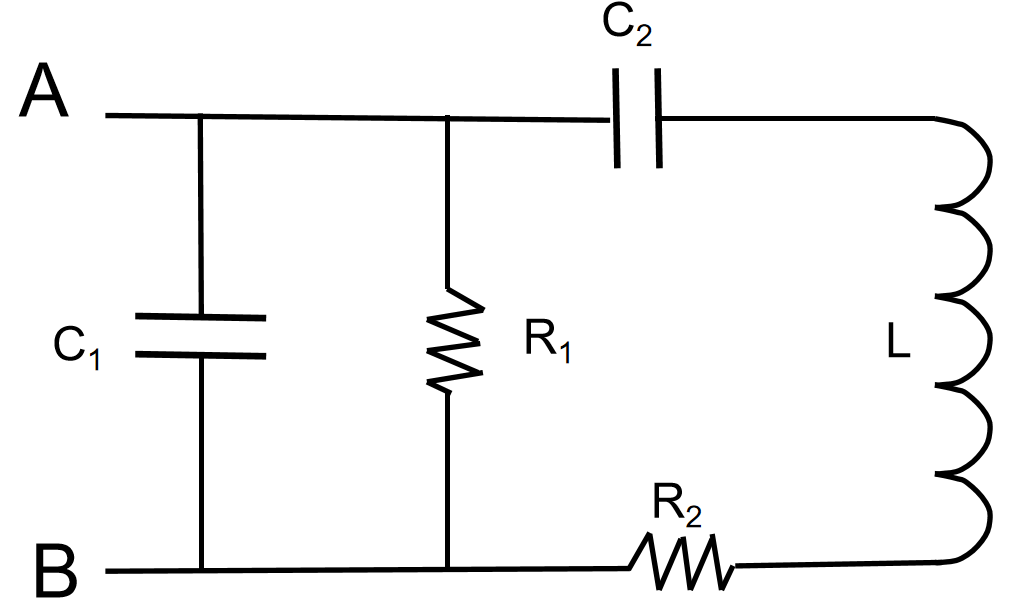
\includegraphics[height=4.25cm]{figure/双压电晶片等效电路.png}
    	\caption{双压电晶片等效电路图}
    	\label{双压电晶片等效电路图}.
    \end{minipage}
    \end{figure}

    双压电晶片如图\ref{双压电晶片示意图}所示,当在AB晶片间施加交流电压时,若片的电场方向与极化方向相同,则起到了增强极化作用的效果,若电场方向与极化方向相反,则对极化作用起到了削弱的效果,利用该原理,可使压电晶片产生与交变电场频率相同的交变形变,当这种形变传递到介质中时,就产生超声波。双压电晶片的等效电路如图\ref{双压电晶片等效电路图}所示。$C_1$为静电电容,$R_1$为陶瓷材料介电损耗并联电阻,$C_2$和$L$为陶瓷材料介电损耗并联电阻,$R_2$为损耗串联电阻\upcite{51单片机超声波测距仪防撞报警倒车雷达设计}。\par

    压电陶瓷晶片有一个固定的谐振频率,即中心频率$f_0$。发射超声波时,施加在其上的脉冲信号频率与固有频率越接近,传感器的分辨率越高。当所用的压电材料不变时,改变压电陶瓷晶片的几何尺寸,就可改变其固有谐振频率。利用这一特性就可制成各种固有频率的超声传感器\upcite{车载可视倒车雷达预警系统的研制16}。
    超声波传感器的结构如图\ref{超声换能器结构图}所示,其主要由金属网、外壳、圆锥形振子、双晶振子、底座和引脚等部分组成 。
    \begin{figure}[!h]
    	\centering
    	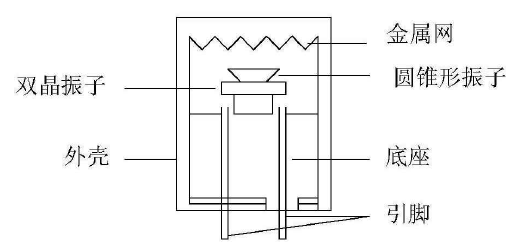
\includegraphics[width=7cm]{figure/超声换能器结构图.png}
    	\caption{超声换能器结构图}
    	\label{超声换能器结构图}
    \end{figure}

    \subsubsection{超声波接近传感器的检测原理}
    \paragraph{连续波相位检测法(CW法))}
    连续波相位检测法的测距原理如图\ref{连续波相位检测法}所示。发射换能器和接收换能器同时发射和接收超声波信号,通过检测信号之间的相位差来获取时间延迟,并计算出传感器与障碍物之间的距离\upcite{面向机器人安全避障的MEMS压电超声接近觉传感器的研究34}。\par
    \begin{figure}[!h]
    	\centering
    	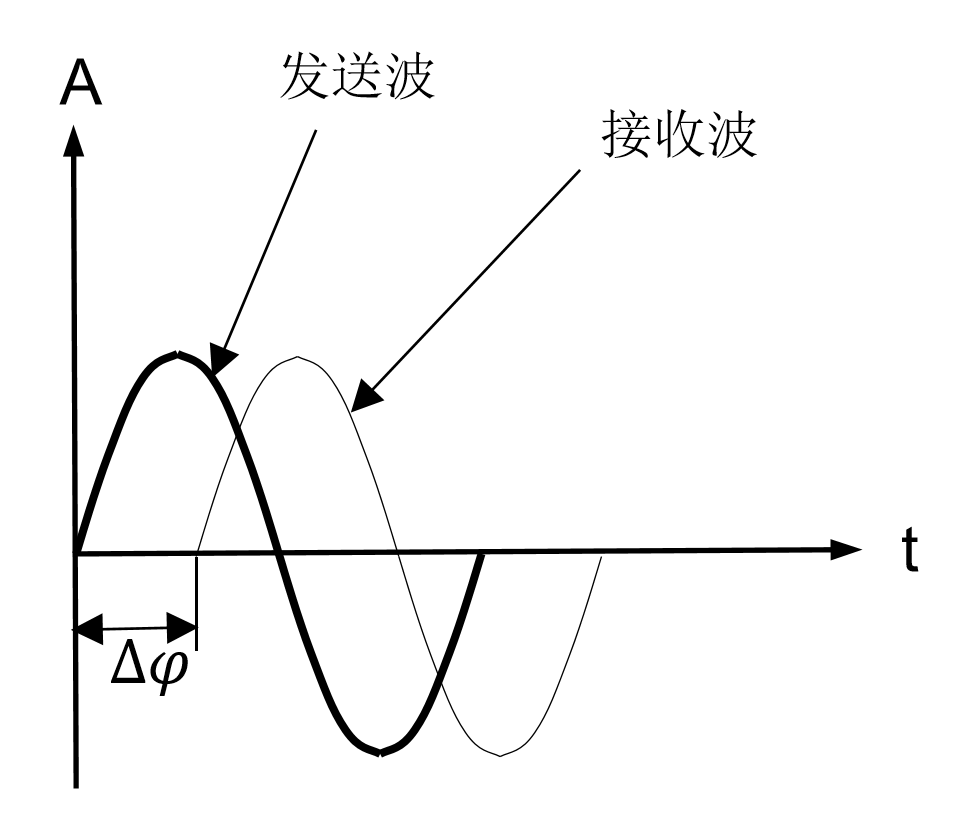
\includegraphics[width=6cm]{figure/连续波相位检测法.png}
    	\caption{连续波相位检测法}
    	\label{连续波相位检测法}
    \end{figure}\par


    假设 发射 的 声 波信 号 为 :
    \begin{equation}
    	u_1=A(x)sin(\omega t + \varphi)
    \end{equation}
式中\quad$\varphi$---初始相位角
接收到的回波信号为:
\begin{equation}
	u_2=A(x)sin(\omega t + \varphi + \omega \cdot{\frac{2D}{c}})
\end{equation}
式中\quad$c$---声速\par
发射声波与回波间的相位差为$\Delta \varphi=\frac{2D}{c}$,传感器与检测物体间的距离D为:
\begin{equation}
	D=\frac{c}{2\omega}\cdot \Delta \varphi=\frac{c}{4\pi f}\cdot(2\pi n + \varphi_i)
\end{equation}
式中\quad$n$---整周期的个数;
\quad$\varphi_i$---不完整周期的相位值。\par
虽然相位检测法的精度比较高,但处理电路的成本也高,需要设计比较复杂的处理电路才能准确地确定回波信号的相位,计算量大\upcite{面向机器人安全避障的MEMS压电超声接近觉传感器的研究35}。\par



    
    \paragraph{飞行时间法}
    飞行时间检测法又称脉冲一回波检测法(如图\ref{飞行时间检测法})。超声换能器发射一组脉冲,在遇到障碍物后脉冲进行反射,换能器在接收到反射回波时,会与发射时刻之间产生时间延迟,该时间延迟称为超声波的飞行时间$t$,飞行时间$t$与声波速度$c$和传播距离$L$有关,即$t=\frac{L}{c}$。
    \begin{figure}[!h]
    	\centering
    	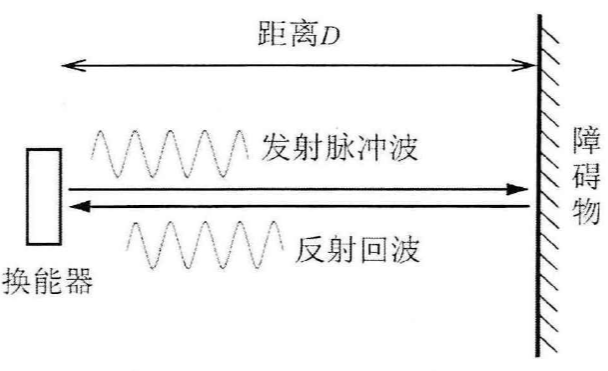
\includegraphics[width=6cm]{figure/飞行时间检测法.png}
    	\caption{飞行时间检测法}
    	\label{飞行时间检测法}
    \end{figure}\par
    飞行时间法最少使用一个换能器便可以实现超声波脉冲的发射和接受,对于自发自收的测距传感器,距离$D$的计算公式为:
    \begin{equation}
    	D=\frac{L}{2}=\frac{ct}{2}
    \end{equation}\par

	采用飞行时间检测法进行障碍物测距,如何简单准确地获得超声波自发射至接收时的飞行时间,是此方法的关键所在。获取飞行时间的方法有很多种,常见的飞行时间法有:互相关函数法、固定阈值法和包络峰值法。\par
	超声波的回波信号相较于发射信号而言,波形基本不变,但在时间上会有一定延迟,因此这两个信号具有相关性。为了准确获取超声波自发射至接收的飞行时间,可以采用相关函数法进行测量。互相关函数法是对超声波的发射信号和回波信号进行互相关函数计算,函数最大值处所对应的时刻就是收发信号相关性最大的时刻,也是回波信号的接收时刻\upcite{面向机器人安全避障的MEMS压电超声接近觉传感器的研究36}。通过计算超声波发射时刻与互相关函数最大值时刻之间的时间差,就可以准确获得超声波的飞行时间。除此之外,固定阈值法和包络峰值法也是常用的飞行时间法。\upcite{面向机器人安全避障的MEMS压电超声接近觉传感器的研究}\par
	固定阈值法是指预先设置一个确定的阈值,当接收的回波信号幅值大于此阈值时,认为此信号幅值所在时刻为回波信号的到达时刻,从而获取超声波的飞行时间。但是在回波信号达到预设阈值时,此时所确定的时刻并不是回波信号的起振时刻,具有一定的时间偏差进行时间补偿将其消除后便可获得飞行时间的估计值。阈值预设大小是固定阈值法用于测量距离的关键因素之一。在固定阈值法中,通过将预设阈值与回波信号的幅值进行比较来判断障碍物距离,而阈值的设置会直接影响到测量结果的精确度。如果阈值设置过高,当障碍物距离较远时,回波信号幅值无法达到阈值大小,导致无法获取飞行时间,从而无法准确测量距离。相反,如果阈值设置过低,噪声信号容易达到阈值大小,造成误触发,导致测量结果不可靠。此外,固定阈值法方法还存在其他问题,例如不同反射距离的回波信号波形幅值大小不同,所造成的时间偏差也不同,简单时间补偿无法获得真实飞行时间,进一步降低了测量结果的精确度。因此,虽然固定阈值法方法简单、易实现、计算量不大,但其精度不高,抗干扰能力差的缺点不能忽视。\par
	包络峰值法是一种常见的获取超声波飞行时间的方法。该方法利用回波信号包络线的峰值所在时刻来获取飞行时间。相比于固定阈值法,该方法更加准确,因为回波信号的幅值会随着传播距离的增加而发生变化,而峰值所在的位置相对回波信号的起振时刻并没有发生变化。此外,回波信号的上升时间与超声波发射信号的频率和周期有关,而与传播距离无关,这种特性也使得包络峰值法可以较好地弥补时间偏差,提高测量精度。值得一提的是,包络峰值法同样存在一些缺点,例如受噪声和杂波的影响较大,需要在实际应用中进行适当的干扰抑制和信号处理。\upcite{面向机器人安全避障的MEMS压电超声接近觉传感器的研究38}。
	       
\subsection{本设计的主要研究内容和论文结构安排}
\subsubsection{主要研究内容}
本设计针对生产线上检测钢化玻璃到位问题,设计了一种稳定性好、灵活性高、应用场景广的超声波接近传感器。
本设计的主要研究内容包括了超声波接近传感器的硬件设计、软件设计和实验设计。\par
硬件设计部分包括了原理图设计和PCB设计,软件设计包括了驱动芯片配置、脉冲信号产生、物体检测三个部分的程序设计以及波形仿真,实验设计部分包括了设计实验进行性能参数测试、稳定性测试和回波特性测试。

\subsubsection{论文结构安排}
本文各章节的主要内容如下:

第二章:提出了超声波接近传感器的总体设计,分为硬件设计、软件设计、实验设计三个部分,初步介绍各个部分的设计流程与方法步骤。然后讲解了在本设计所涉及到的检测原理。

第三章:对传感器的硬件电路设计进行研究,介绍了原理图设计和PCB设计的设计过程。原理图部分的设计分为三部分,分别为:超声波接近传感器控制电路设计、TUSS4470芯片外围电路设计、检测计数电路设计。PCB设计部分主要介绍了TUSS4470外围电路PCB设计,讲解了在PCB设计过程中遵循的几大原则,用于减小各类信号相互之间的干扰,包括了电容、二极管等器件摆放位置优先级,分离接地,铺铜规则等。

第四章:对传感器的软件设计进行研究,首先讲解了传感器所采取的检测策略,然后进行程序的总体设计,根据功能将程序分为了四个模块,分别为:控制模块、SPI模块、脉冲产生模块和检测计数模块。之后分别详细讲解了各个模块的功能、实现原理以及程序流程图。在完成了程序设计方面的工作后,又介绍了如何搭建仿真环境进行程序仿真模拟,最后,给出了仿真模拟后的波形图,并进行了分析。

第五章:设计实验测试传感器的性能以及检测策略的可行性。首先讲解了实物的焊接与调试流程,给出了调试过程中所测得的各引脚波形,然后介绍了实验所用的实验器材,包括虚拟示波器、直尺、各种板材等。最后进行实验,测试了传感器的性能参数、稳定性以及回波特性,给出了实验的结果以及后续分析。

第六章:对本设计存在的不足进行总结,提出了改进的方向,并且进行了对未来的展望。


    \subsection{本章小结}
    本章绪论主要介绍了超声波接近传感器的研究背景和意义,在研究背景中介绍了超声波接近传感器总体的发展情况以及国内外研究现状,然后引出本设计的研究意义是为了设计精度高、稳定性好的传感器。在第二节主要介绍了传感器主要涉及到的原理,包括超声波振幅衰减原理、超声换能器发射脉冲与检测回波信号的原理以及在本设计中的检测原理。在本章的最后一节,则是介绍了本设计的主要研究内容和论文结构安排
    ,并且简单介绍了后几章所包含的内容。
%------------------第三章---------------------------
    \newpage
	\section{超声波接近传感器硬件设计}
	
    \subsection{超声波接近传感器控制电路设计}
    本设计中所使用的CPLD芯片型号为EPM240T100C5N,涉及到的控制电路较简单,在最小系统板的基础上,增加了检测计数电路和TUSS4470外围电路。如图\ref{传感器整体原理图}为传感器整体的原理图,其中主要包括了电源模块、JTAG下载模块、检测计数模块、时钟模块以及复位模块\upcite{CPLD芯片设计指南}。电源
    \begin{figure}[ht]
        \centering
        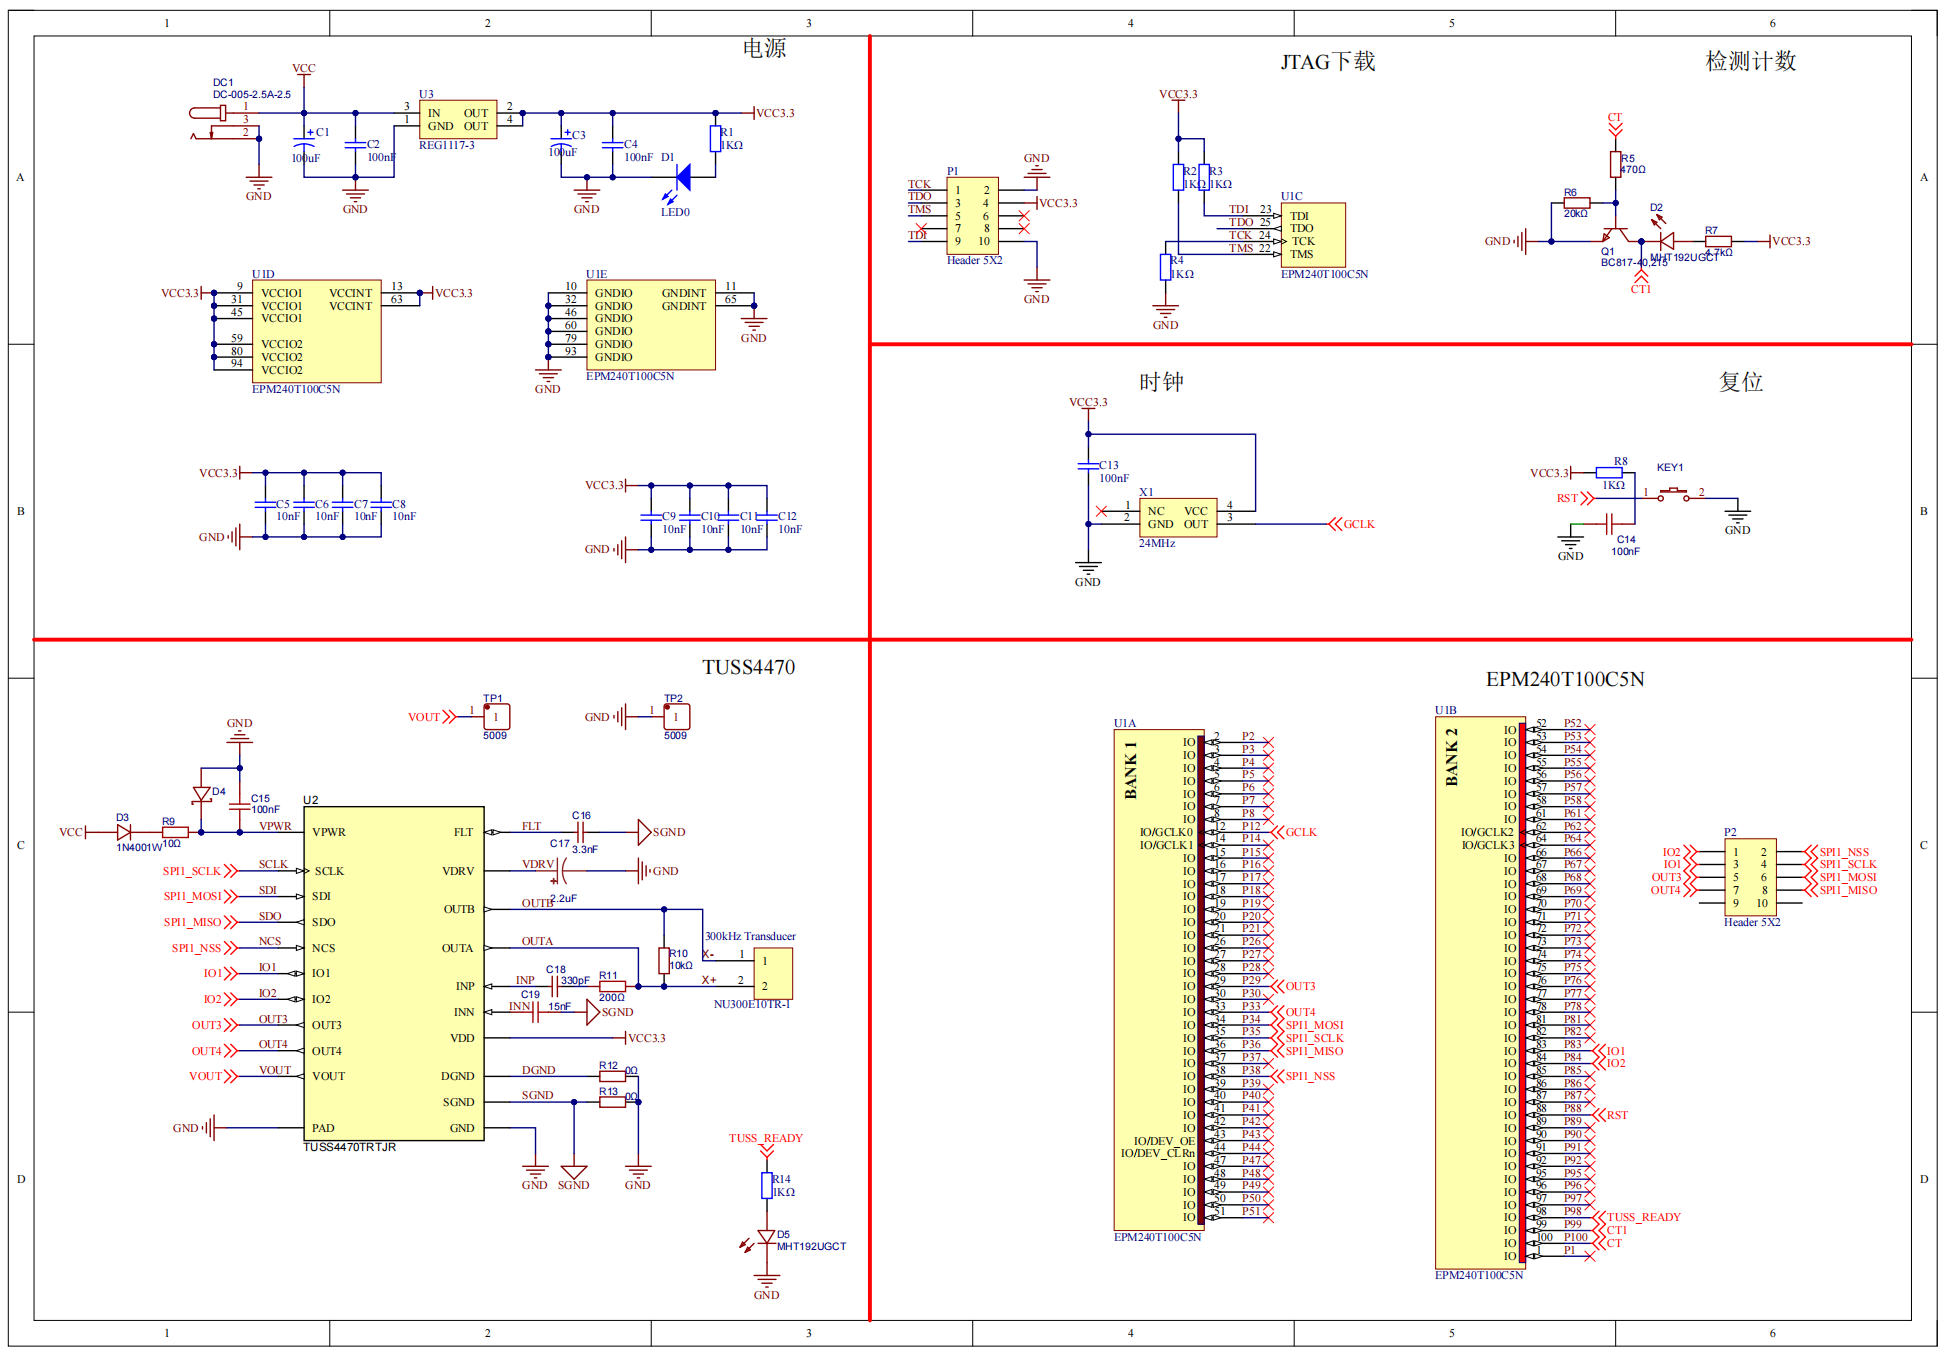
\includegraphics[width=12cm]{figure/Overall circuit.png}
        \caption{传感器整体原理图}
        \label{传感器整体原理图}
    \end{figure}
    \subsubsection{电源模块}
      根据查找芯片手册,可得知EPM240T100C5N的控制电压为:
    TUSS4470芯片的控制电压为3.3V,
    超声探头的驱动电压为:5V-30V\upcite{超声探头手册}。
    可得出电源的设计方案。电源由DC接口、降压芯片、滤波电容组成,可得到12V以及3.3V的电压为各模块供电。电源模块中还包括了一个红色LED指示灯,当模块正常工作时,LED灯就会被点亮。
    
    \subsubsection{JTAG下载模块}
    JTAG(Joint Test Action Group) 下载模块是一种用于编程和调试数字电路和嵌入式系统的通信接口。它通常由三个主要部分组成:JTAG控制器、JTAG下载模块和目标设备。JTAG下载模块的主要作用是将编译后的程序通过JTAG接口下载到目标设备中。在本设计中JTAG主要用于下载烧录调试MCU代码。
    图\ref{JTAG下载模块电路图}左侧为JTAG接头,用于连接下载器,右侧为MCU芯片的连接图其中TCK引脚为测试时钟,
    TDI引脚为测试数据输入,
TDO引脚为测试数据输出,
TMS为测试模式选择,
因为只有一条数据线,通信协议有必要像其他串行设备接口,如SPI一样为串列传输。时钟由TCK引脚输入。配置是通过TMS引脚采用状态机的形式一次操作一位来实现的。每一位数据在每个TCK时钟脉冲下分别由TDI和TDO引脚传入或传出。可以通过加载不同的命令模式来读取芯片的标识,对输入引脚采样,驱动(或悬空)输出引脚,操控芯片功能,或者旁路(将TDI与TDO连通以在逻辑上短接多个芯片的链路)。
    \begin{figure}[ht]
        \centering
        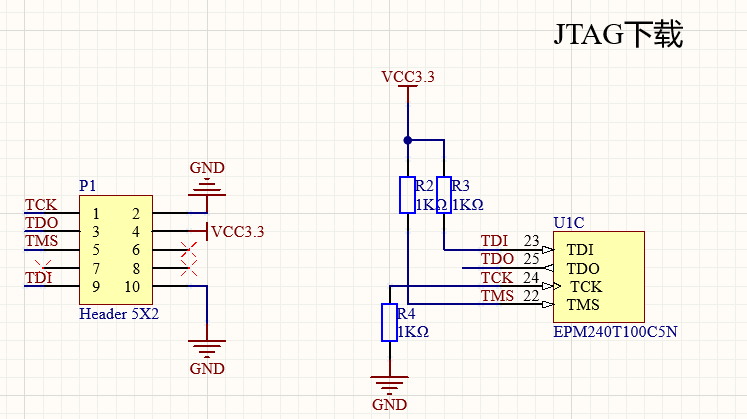
\includegraphics[width=7cm]{figure/JTAG download circuit.png}
        \caption{JTAG下载模块电路图}
        \label{JTAG下载模块电路图}
    \end{figure}
    
    \subsubsection{检测计数模块}
    检测计数模块的功能在于,亮灯提示钢化玻璃到位,并对经过的玻璃进行计数。如图\ref{检测计数模块电路图},CT引脚为MCU输出信号,当程序确定检测到物体后,CT引脚电压拉高,LED灯亮,当物体离开检测范围后,LED等灯灭。CT1引脚则是作为MCU的输入信号,当检测到一次物体后,CT1发出一次脉冲信号,计数加一,以此来实现计数功能。
    \begin{figure}[ht]
        \centering
        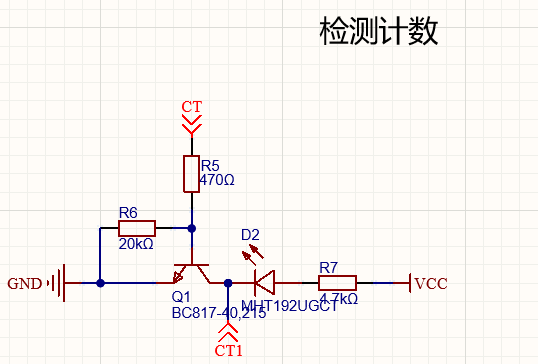
\includegraphics[width=7cm]{figure/detection count circuit.png}
        \caption{检测计数模块电路图}
        \label{检测计数模块电路图}
    \end{figure}
\newpage
       \subsubsection{超声波接近传感器控制电路PCB设计}
       在完成控制电路原理图的设计后,就将进行PCB部分的设计。如图\ref{超声波接近传感器整体PCB设计}为传感器PCB整体设计图,图\ref{超声波接近传感器控制电路PCB设计}为控制电路PCB的设计。
\begin{figure}[ht]
	\centering
	\subfloat[超声波接近传感器整体PCB设计]{
		\begin{minipage}[b]{0.5\textwidth}
			\centering
			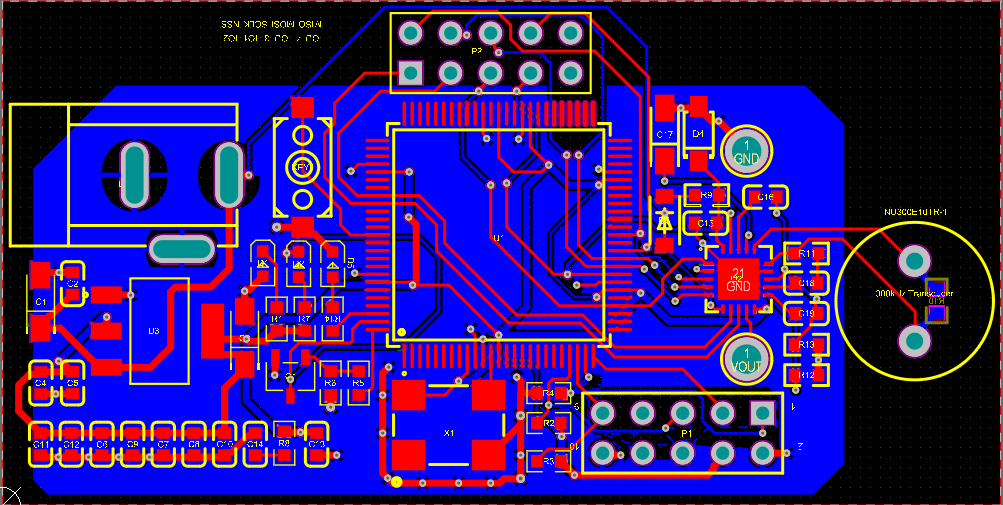
\includegraphics[height=4.5cm]{figure/overall pcb.png}
		\end{minipage}
		\label{超声波接近传感器整体PCB设计}
	}
	\subfloat[超声波接近传感器控制电路PCB设计]{
		\begin{minipage}[b]{0.5\textwidth}
			\centering
			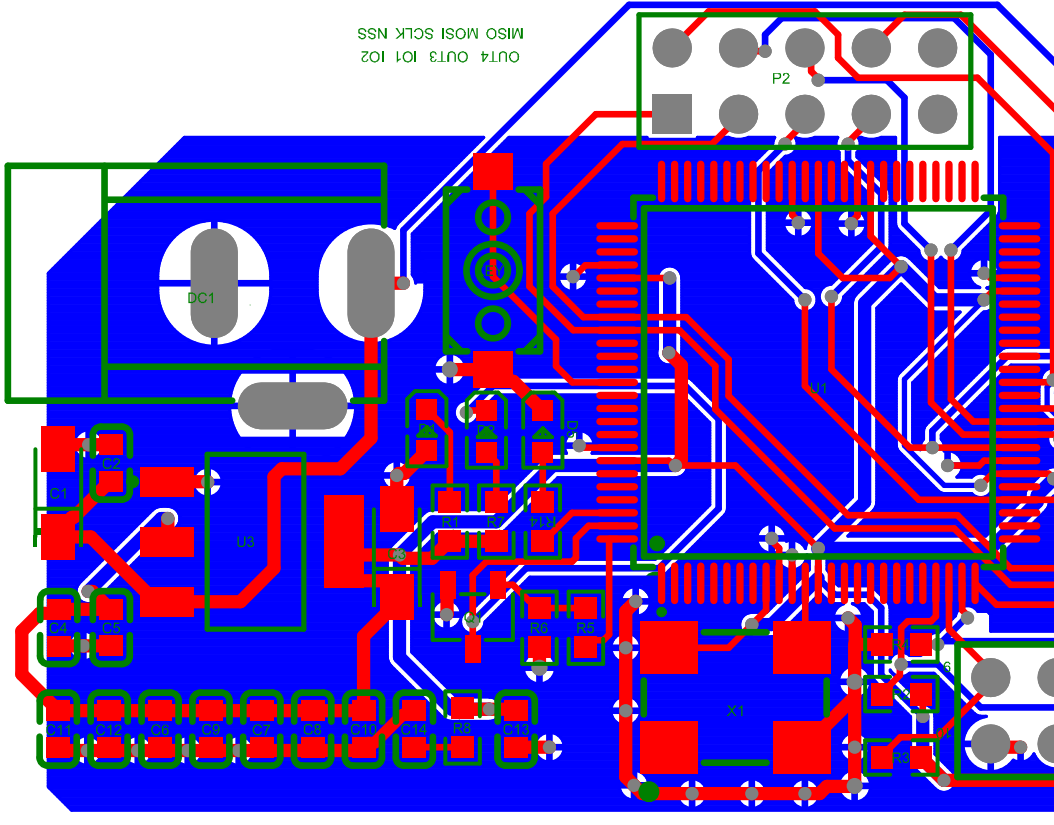
\includegraphics[height=4.5cm]{figure/cpld pcb.png}
		\end{minipage}
		\label{超声波接近传感器控制电路PCB设计}
	}
	\caption{超声波接近传感器PCB设计}
	\label{超声波接近传感器PCB设计}
\end{figure}
   \paragraph{线宽}
   对于功率较大的部分如电源、超声换能器驱动部分,需要对布线进行加宽处理,避免因发热而影响电路板正常工作,甚至产生损坏。\par
   \paragraph{时钟包地处理}
   对于速率较低的时钟,需进行包地处理。包地的作用主要有两点:一是拉开与其他信号的距离,从而减小干扰;二作为自身参考和屏蔽。包地处理还需要在地线上等间距打过孔。
  
 	\newpage
    \subsection{TUSS4470芯片外围电路}
    
    
    \begin{figure}[ht]
		\centering
		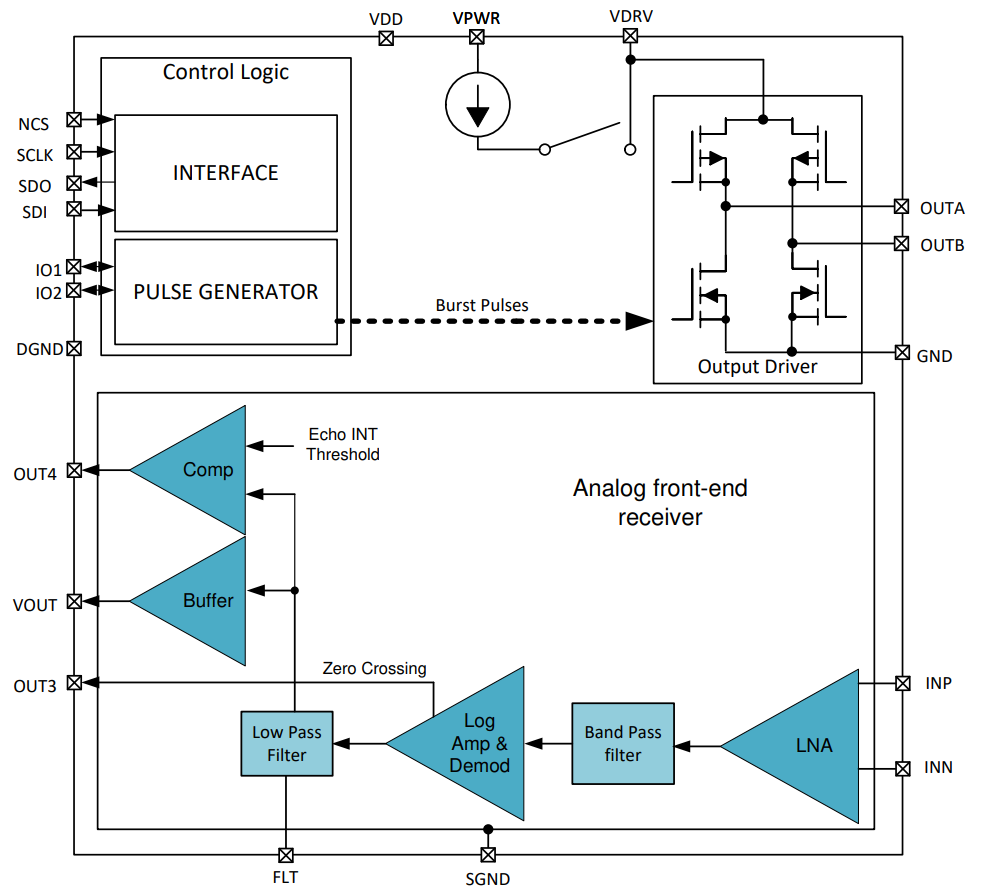
\includegraphics[width=12cm]{figure/Function Block Diagram.png}
		\caption{TUSS4470芯片功能框图}
		\label{TUSS4470芯片功能框图}%文中引用该图片代号
\end{figure}
 图\ref{TUSS4470芯片功能框图}为TUSS4470驱动芯片的整体功能框图\upcite{TUSS4470芯片手册},以此作为外围电路设计的参考资料。如图所示,芯片按照功能可分为逻辑控制、输出驱动、回波接收三个部分。其中逻辑控制部分又分为SPI通信和脉冲发生模块,SPI通信模块用于接收MCU芯片发送的芯片配置数据,脉冲发生模块的两个引脚IO1、IO2连接MCU芯片作为脉冲发生控制引脚,根据芯片不同的IO模式,两个引脚配合产生指定脉宽、脉冲数的脉冲信号;输出驱动模块的OUTA、OUTB引脚直接连接超声换能器,VDRV引脚连接外部电容,VPWR可对电容充电,在VDRV到达设定电压值后,VPWR停止对VDRV供电,这使得超声换能器的驱动电压可以保持在设定值,以此保证发出脉冲的声压水平可以稳定在一定水平,从而保证发射出稳定的脉冲波(其中VDRV的设定电压可通过SPI对芯片进行配置);回波接收模块的作用在于:对回波信号进行处理,输出可供MCU进行检测判断的信号其中INP、INN引脚连接超声波换能器的正负端,FLT连接外部电容作为低通滤波器对回波信号进行滤波处理。OUT3引脚内部连接至模块中的对数解调模块,当回波信号在模块内进完成放大进行解调时,将某阶段信号作为零点,输出过零信号,以验证接收信号的频率, 提高对其他信号的抗干扰性。OUT4作为检测到位的指示信号,当VOUT输出电压超过芯片配置数据中设定的阈值时,OUT4拉高。(VOUT引脚的电压值由公式\ref{VOUT公式}决定)。
  
    \begin{equation}
        V_{OUT}=G_{VOUT} \cdot SL_{LOG}\cdot20log_{10}(\frac{G_{LNA} \cdot G_{BPF} \cdot V_{IN}}{INT_{LOG} \cdot K_X})
        \label{VOUT公式}
    \end{equation}
式中\quad $G_{VOUT}$---对数放大器斜率增益调整(Slope or gain adjustment);\par
\quad$SL_{LOG}$---对数运算放大器斜率调整(slope of logarithmicamplifier);\par
\quad$G_{LNA}$---回波增益;\par
\quad$G_{BPF}$---$0.9v/v$;\par
\quad$V_{IN}$---INN引脚输入;\par
\quad$INT_{LOG}$---对数放大器截距( logarithmic amplifier intercept);\par
\quad$K_X$---对数截距平差(log intercept adjustment)\par
    回波接收模块的详细工作框图如图\ref{回波接收模块}所示。
    \begin{figure}[ht]
        \centering
        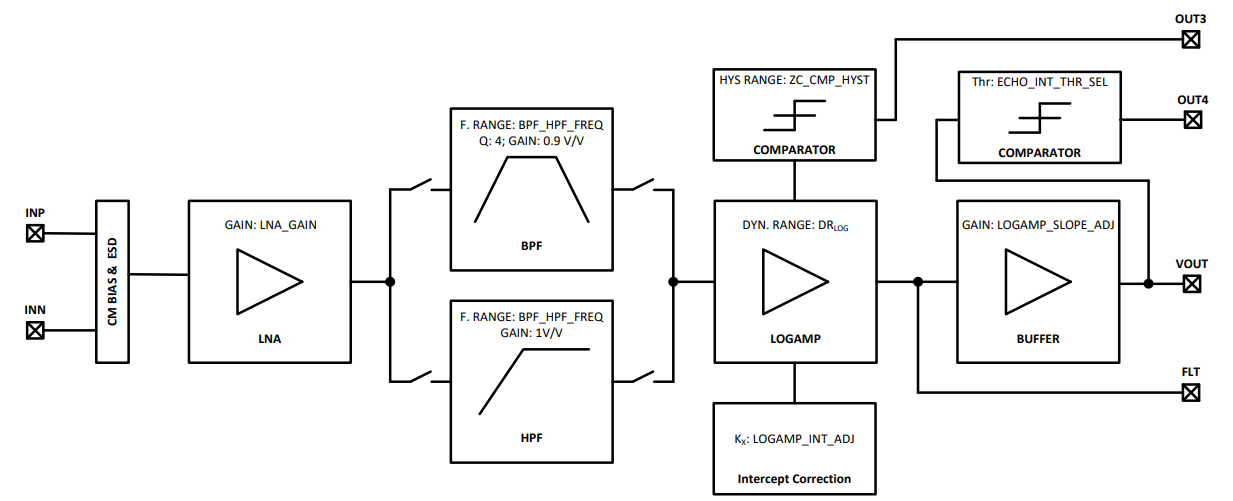
\includegraphics[width=10cm]{figure/Analog Front-End Block Diagram.png}
        \caption{回波接收模块}
        \label{回波接收模块}
    \end{figure}\par

    参考芯片手册相关内容,进行了TUSS4470芯片外围电路的设计,如图\ref{TUSS4470芯片外围电路}所示。
    \begin{figure}[!h]
        \centering
        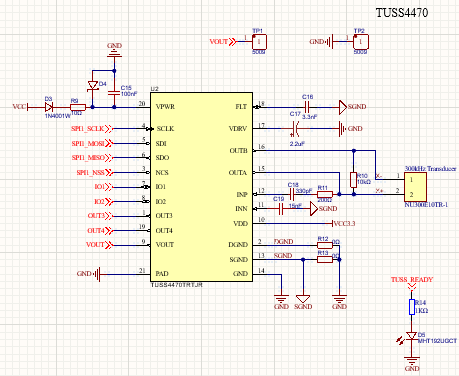
\includegraphics[width=9cm]{figure/TUSS4470 peripheral circuit.png}
        \caption{TUSS4470芯片外围电路}
        \label{TUSS4470芯片外围电路}
    \end{figure}
\newpage
    \subsubsection{VPWR引脚电路}
    VPWR引脚输入电压范围为5V到36V,TUSS4470设备可能受到电池瞬变和反向电流的影响,因此采用外部组件保护芯片十分必要。图\ref{VPWR引脚}中除了靠近引脚的电容C15,二极管D3、D4和电阻R9就起到了保护芯片的作用。
     \begin{figure}[ht]
    	\centering
    	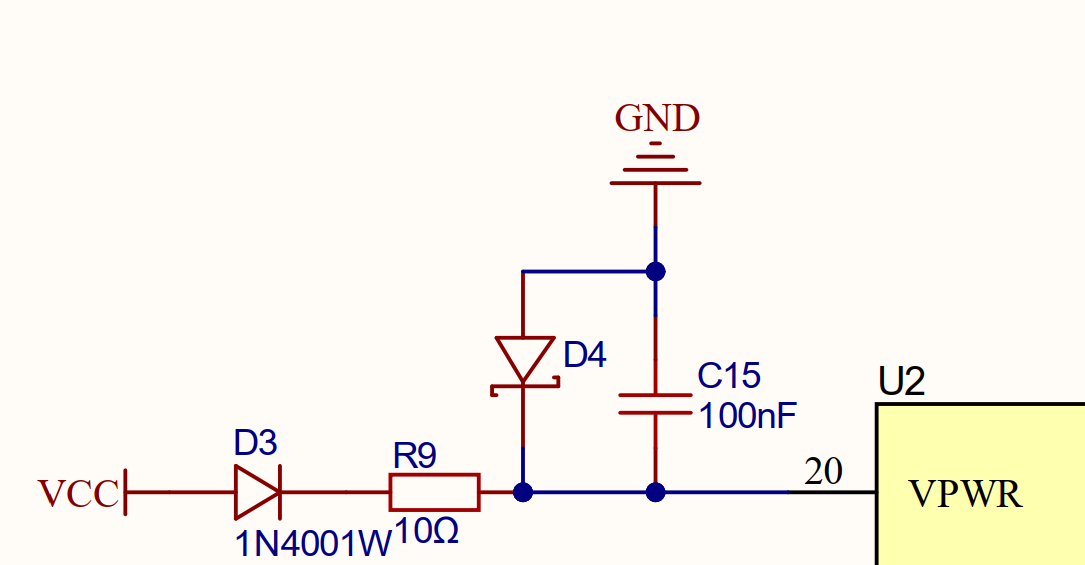
\includegraphics[width=10cm]{figure/VPWR PIN.png}
    	\caption{VPWR引脚电路}
    	\label{VPWR引脚}
    \end{figure}
        \subsubsection{FLT外接滤波电容}
    FLT引脚外接滤波电容,对应图\ref{TUSS4470芯片功能框图}回波检测模块中的低通滤波器。该滤波电容的作用在于,去除对数放大器输出中的高频信号,使解调包络信号有足够的峰值保持时间,而截止频率的大小则由FLT引脚的阻抗以及外接电容的电容量所决定,该电容虽然可以抑制高频信号的波动,但同样会减缓信号的响应速度。大电容量可以使VOUT引脚输出的电压峰值变化减小,并且减缓上升下降到峰值的时间,而最优电容量则需在应用中不断进行优化。本设计初步使用电容量为3.3nF的电容。
    \subsubsection{VDRV引脚电路}    
    VDRV引脚连接外部电容,TUSS4470芯片通过VPWR引脚为外部的电容充电,当其达到设定电压时则停止充电,此时该电容将为超声换能器H桥驱动电路供能。
     \subsubsection{超声换能器驱动电路}
    在TUSS4470的芯片手册中,超声换能器有四种不同的驱动方式,不同驱动方式产生脉冲的方式也不同,本设计中采用最典型的HALF\_BRG\_MODE\_0来进行驱动,如图\ref{参考配置方式}为参考配置方式,图\ref{实际配置方式}为本设计中所采用的方式。
    
\begin{figure}[ht]
	\centering
	\subfloat[参考配置方式]{
		\begin{minipage}[b]{0.5\textwidth}
			\centering
			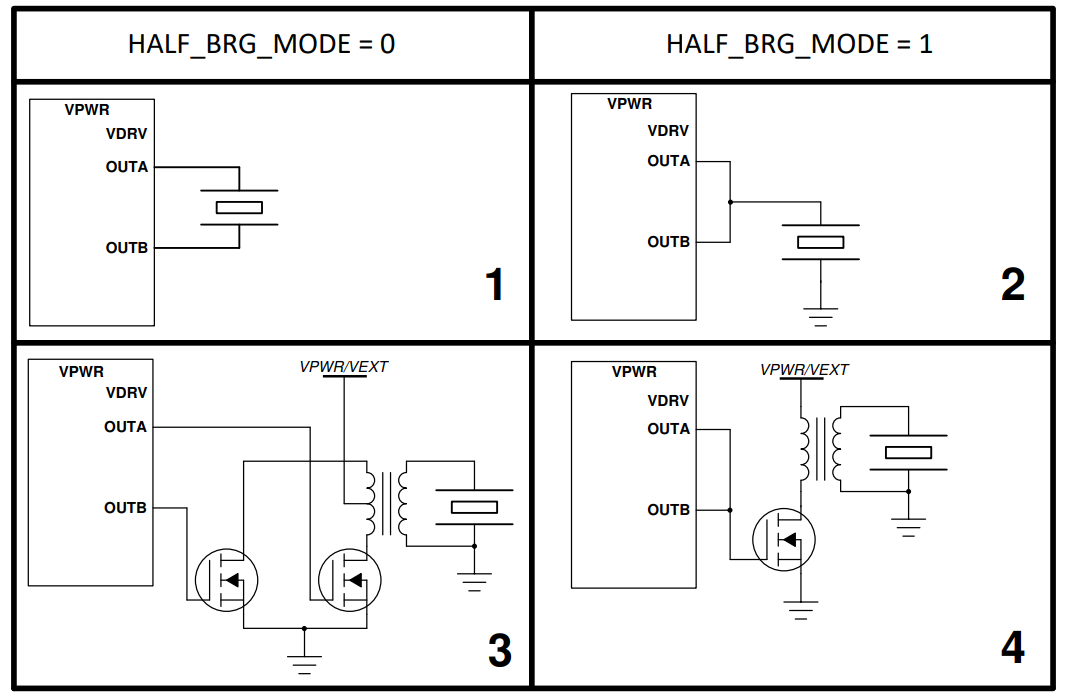
\includegraphics[height=4.5cm]{figure/TUSS4470 Transducer Drive Options.png}
		\end{minipage}
		\label{参考配置方式}
	}
	\subfloat[实际配置方式]{
		\begin{minipage}[b]{0.5\textwidth}
			\centering
			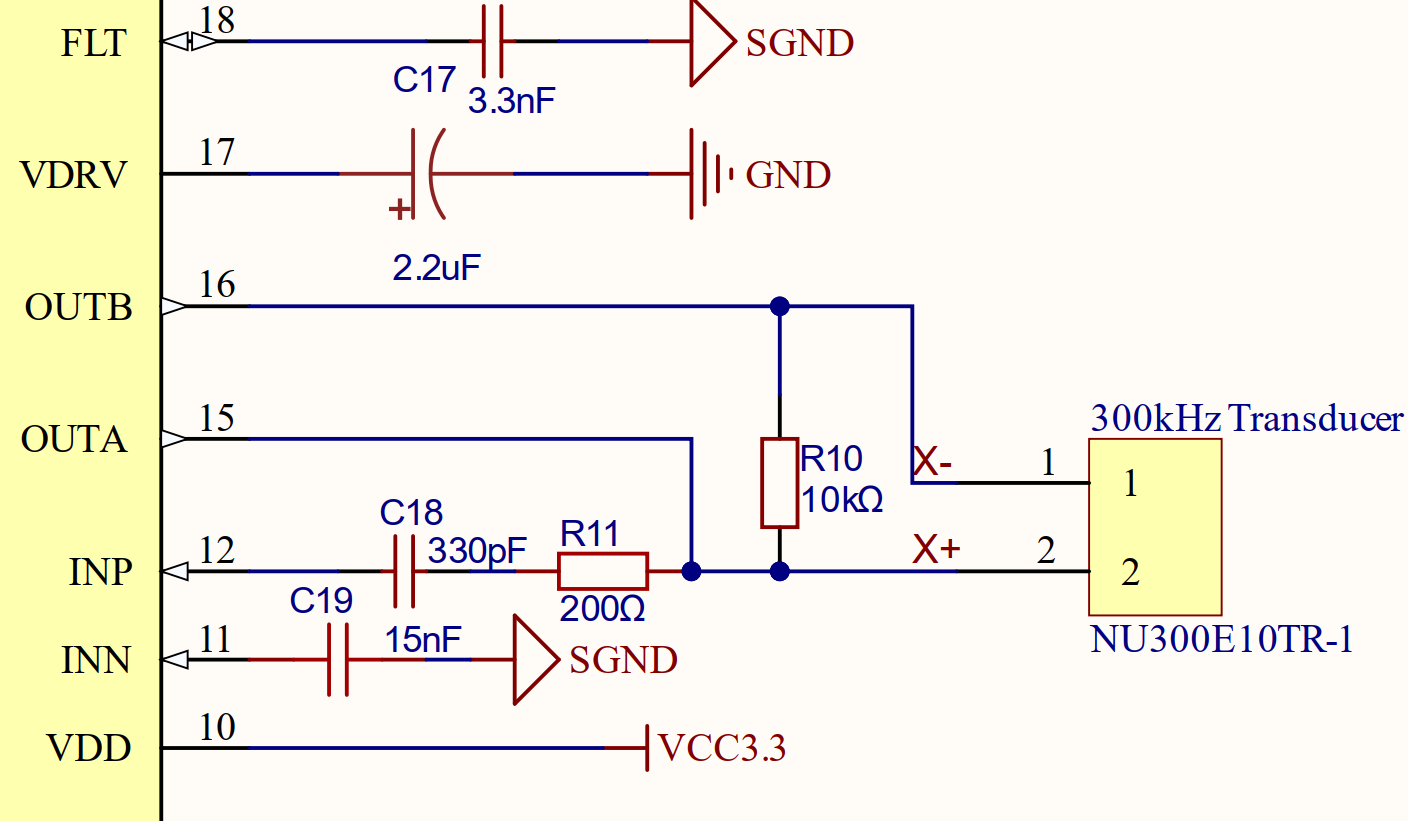
\includegraphics[height=4.5cm]{figure/OUTA PIN.png}
		\end{minipage}
		\label{实际配置方式}
	}
	\caption{超声换能器驱动电路设计}
	\label{超声换能器驱动电路设计}
\end{figure}
    \subsubsection{芯片配置指示电路}
    CPLD芯片通过SPI协议向TUSS4470芯片发送配置数据,并接收其反馈回数据。在芯片返回的数据当中,有一位的状态位用来反映芯片是否准备就绪,当芯片准备就绪后该位置1,可供MCU进行下一步的工作。如图为芯片配置指示电路,当芯片配置就绪后,MCU该引脚拉高,LED灯亮,用来指示芯片的配置状态。
    \subsubsection{分离接地电路}
    由于外围电路中包含多种类型的信号,例如VPWR引脚的电源信号,VOUT引脚的模拟信号,VOUT引脚的模拟信号,SCLK等引脚的数字信号。当产生数字信号的引脚产生脉冲时,其变换速度较快,将会在数字地产生较大的噪声;而模拟信号又容易受到外接的干扰,如果将数字信号和模拟信号直接接入同一个大地,将会严重影响模拟信号的准确性,对于超声波传感器而言,是非常致命的。本设计在原理图设计的过程中便解决了不同类型分离接地\upcite{分离接地}的问题,采用的方法是:先将不同类型的信号连接到0$\Omega$电阻,再连接到大地,0$\Omega$电阻相当于很窄的电容通道,能够有效的限制环路电流,使噪声得到抑制。起分离接地作用的电路如\ref{分离接地电路}所示。
     \begin{figure}[!h]
        \centering
        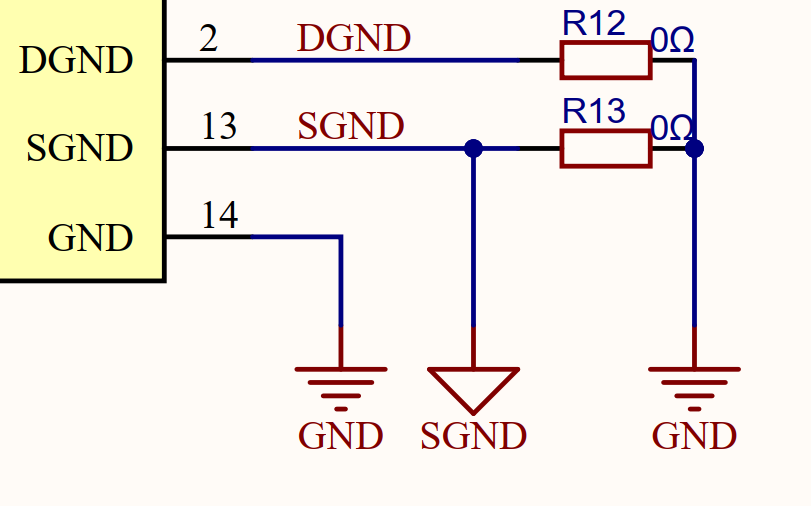
\includegraphics[width=7cm]{figure/seperate ground.png}
        \caption{分离接地电路}
        \label{分离接地电路}
    \end{figure}
	\subsubsection{TUSS4479芯片外围电路PCB设计}
    由于本设计中涉及到的信号类型较多,包括了数字信号、模拟信号、高频信号、大功率信号,各信号间会存在较大的干扰,因此在布线过程中将各信号分离十分重要,直接关系到传感器的稳定性和精度。如图\ref{TUSS4470芯片外围电路PCB设计}为TUSS4470芯片外围电路PCB设计,图\ref{TUSS4470芯片引脚图}为芯片对应的引脚图。本设计采用两层板来完成布线。
  \begin{figure}[!h]
   		\begin{minipage}[t]{0.5\linewidth}
  			\centering
  			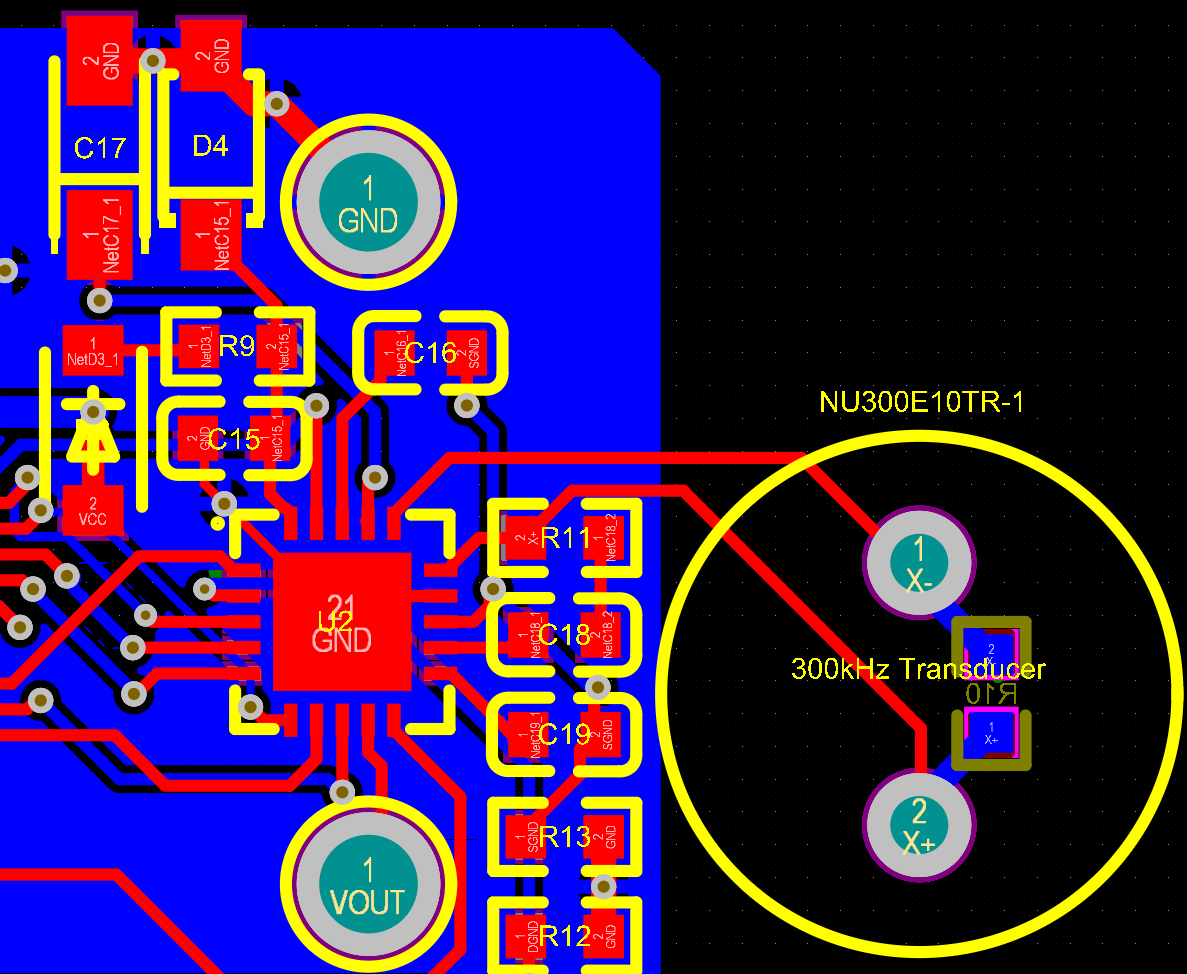
\includegraphics[height=5cm]{figure/TUSS4470 pcb.png}
  			\caption{TUSS4470芯片外围电路PCB设计}
  			\label{TUSS4470芯片外围电路PCB设计}
  		\end{minipage}
   		\begin{minipage}[t]{0.5\linewidth}
  			\centering
  			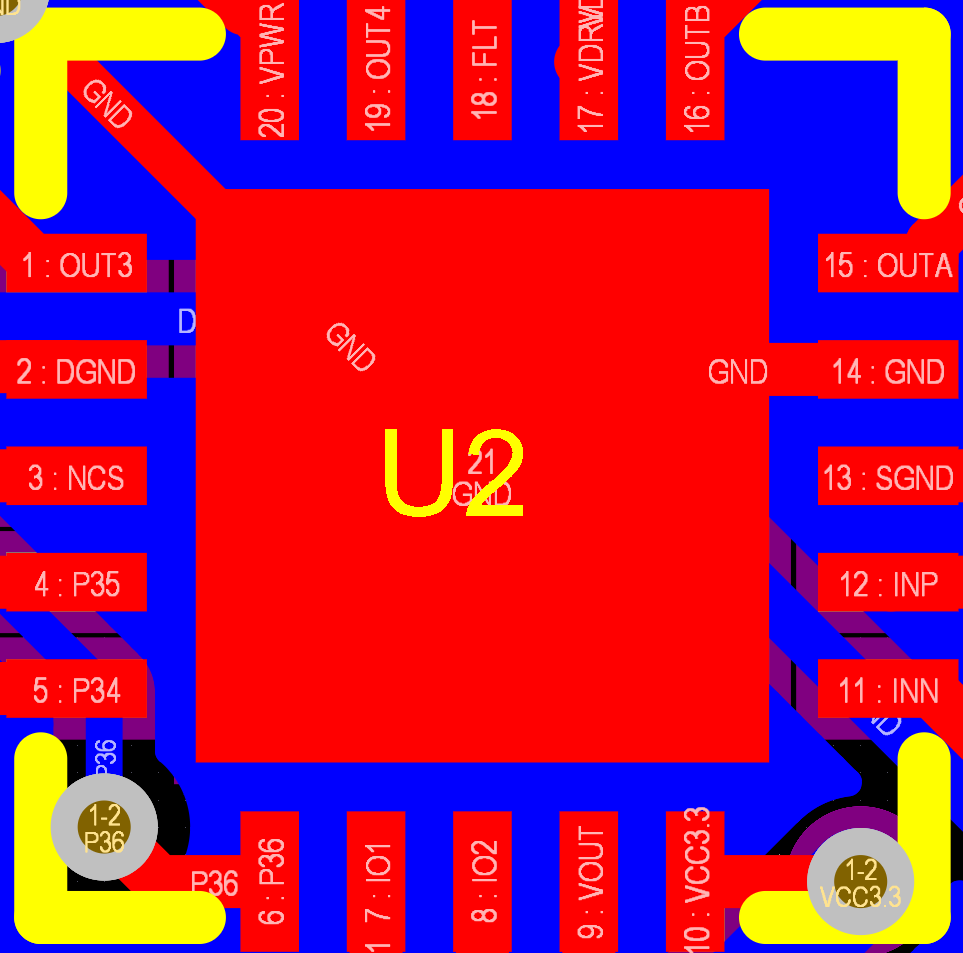
\includegraphics[height=5cm]{figure/TUSS4470 PIN.png}
  			\caption{TUSS4470芯片引脚图}
  			\label{TUSS4470芯片引脚图}
  		\end{minipage}  		 
  \end{figure}\par
    在TUSS4470驱动芯片的PCB设计过程中,最重要的就是将芯片的电源信号、数字信号以及模拟信号进行分离。参考芯片手册\upcite{TUSS4470芯片手册},在布线时考虑到了如下事项。\par
    \paragraph{各类信号分离接地}
    在连接到主地前,数字接地、传感器接地、回波接地都要先通过0$\Omega$电阻或者铜迹线,如图\ref{分离接地电路},本设计在原理图设计时采用了0$\Omega$电阻的方式来实现分离接地,因此在布线时就不需要考虑该问题。
     \paragraph{回波接收引脚}
    INN、INP引脚作为回波信号的接收引脚,对噪声干扰十分敏感,所以其布线必须要短且直,并且保证INN引脚的电容尽量靠近芯片引脚,以减少干扰,但考虑到后续需手工焊接,电容与芯片引脚间仍要保持一定的间隙,以减小手工焊接的难度。假设不考虑测试成本,采用贴片工艺,电容与芯片引脚间的距离还可再进一步减小,以获得到具有更高稳定性的回波信号。
    \paragraph{VOUT引脚}
    VOUT引脚作为模拟信号输出端,与外界的连线应该尽量短直,避免产生寄生效应\upcite{寄生效应},以及外部噪声干扰引起的噪声耦合。\par
    \paragraph{超声换能器驱动}
    芯片与OUTA、OUTB引脚间的布线应尽可能短且直,以保证发出脉冲信号的质量,从而提高传感器的精度。考虑到两个引脚输出的是大功率、高频率的模拟信号,连接到两引脚的线宽应不能太小。\par
    \paragraph{VPWR引脚}
        根据芯片手册推荐,VPWR的解调电容应尽可能靠近引脚。\par
     \paragraph{信号分离}
     数字信号引脚如TXD、RXD、 SCLK、 NCS、IO1、 IO2、 OUT3、OUT4应远离模拟信号引脚,避免信号间的干扰。\par
\subsection{本章小结}
本章主要介绍了超声波接近传感器硬件部分的设计,首先介绍了超声波接近传感器控制电路的设计,该部分包括了原理图设计和PCB设计,重点讲解了JTAG下载模块的设计和时钟包地处理。然后又详细介绍了TUSS4470芯片外围电路的设计,该部分讲解了各管脚连接器件的选型以及PCB设计过程中需要注意的事项,原理图设计部分详细介绍了VPWR引脚、VDRV引脚以及各类信号分离接地处理的设计,而PCB设计部分则详细介绍了各类器件的布局原则,以减少信号间的相互干扰。\par
至此已介绍完成了超声波接近传感器原理图设计和PCB设计部分的工作,下一章将详细讲解传感器的软件设计部分。

      
    
    
    
%------------------第三章---------------------------
    \newpage
	\section{超声波接近传感器硬件设计}
	
    \subsection{超声波接近传感器控制电路设计}
    本设计中所使用的CPLD芯片型号为EPM240T100C5N,涉及到的控制电路较简单,在最小系统板的基础上,增加了检测计数电路和TUSS4470外围电路。如图\ref{传感器整体原理图}为传感器整体的原理图,其中主要包括了电源模块、JTAG下载模块、检测计数模块、时钟模块以及复位模块\upcite{CPLD芯片设计指南}。电源
    \begin{figure}[ht]
        \centering
        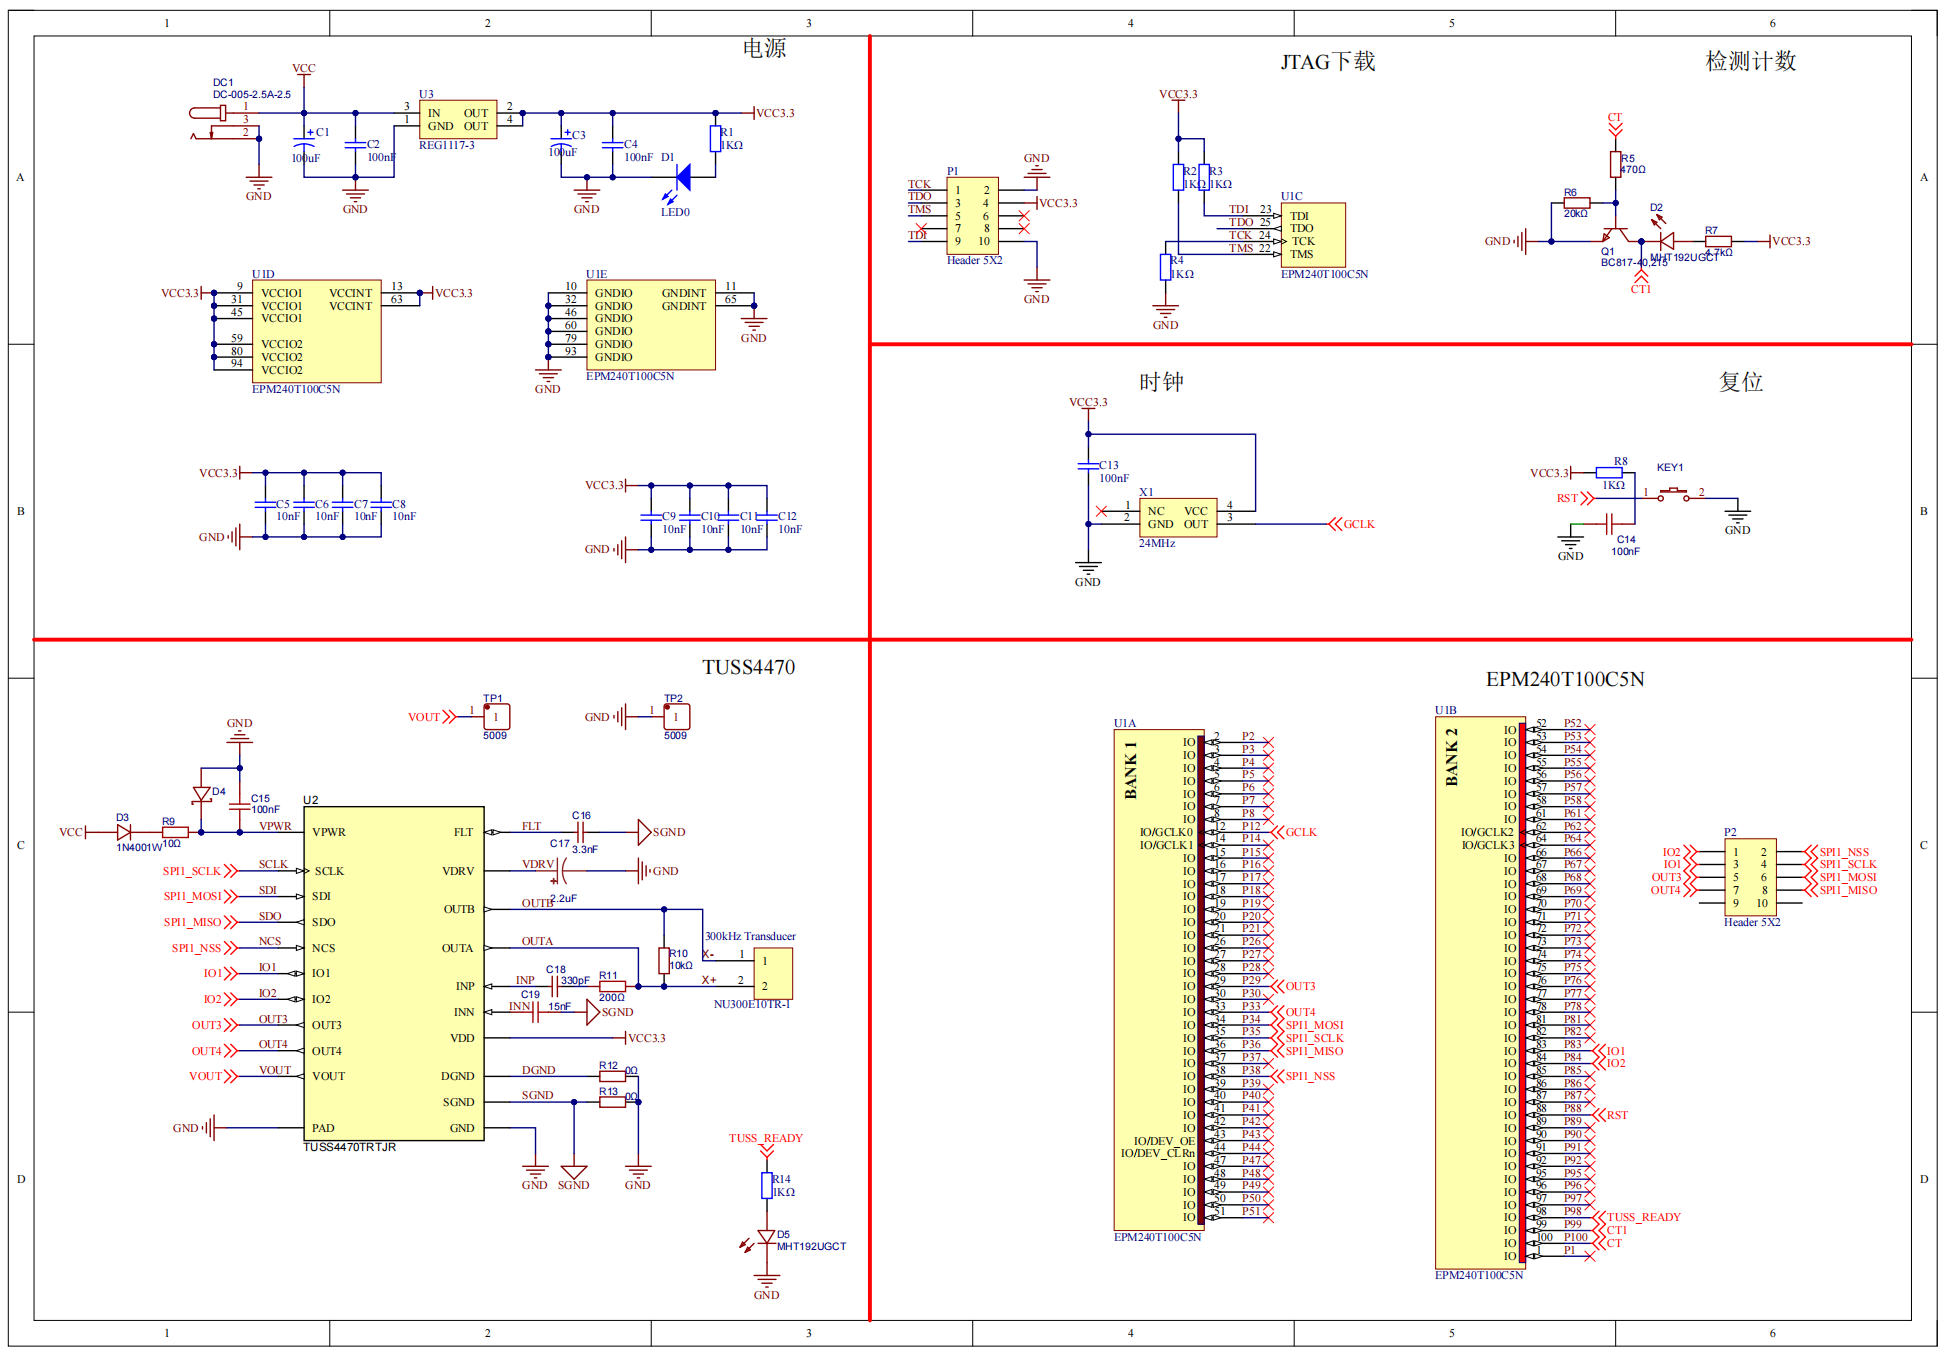
\includegraphics[width=12cm]{figure/Overall circuit.png}
        \caption{传感器整体原理图}
        \label{传感器整体原理图}
    \end{figure}
    \subsubsection{电源模块}
      根据查找芯片手册,可得知EPM240T100C5N的控制电压为:
    TUSS4470芯片的控制电压为3.3V,
    超声探头的驱动电压为:5V-30V\upcite{超声探头手册}。
    可得出电源的设计方案。电源由DC接口、降压芯片、滤波电容组成,可得到12V以及3.3V的电压为各模块供电。电源模块中还包括了一个红色LED指示灯,当模块正常工作时,LED灯就会被点亮。
    
    \subsubsection{JTAG下载模块}
    JTAG(Joint Test Action Group) 下载模块是一种用于编程和调试数字电路和嵌入式系统的通信接口。它通常由三个主要部分组成:JTAG控制器、JTAG下载模块和目标设备。JTAG下载模块的主要作用是将编译后的程序通过JTAG接口下载到目标设备中。在本设计中JTAG主要用于下载烧录调试MCU代码。
    图\ref{JTAG下载模块电路图}左侧为JTAG接头,用于连接下载器,右侧为MCU芯片的连接图其中TCK引脚为测试时钟,
    TDI引脚为测试数据输入,
TDO引脚为测试数据输出,
TMS为测试模式选择,
因为只有一条数据线,通信协议有必要像其他串行设备接口,如SPI一样为串列传输。时钟由TCK引脚输入。配置是通过TMS引脚采用状态机的形式一次操作一位来实现的。每一位数据在每个TCK时钟脉冲下分别由TDI和TDO引脚传入或传出。可以通过加载不同的命令模式来读取芯片的标识,对输入引脚采样,驱动(或悬空)输出引脚,操控芯片功能,或者旁路(将TDI与TDO连通以在逻辑上短接多个芯片的链路)。
    \begin{figure}[ht]
        \centering
        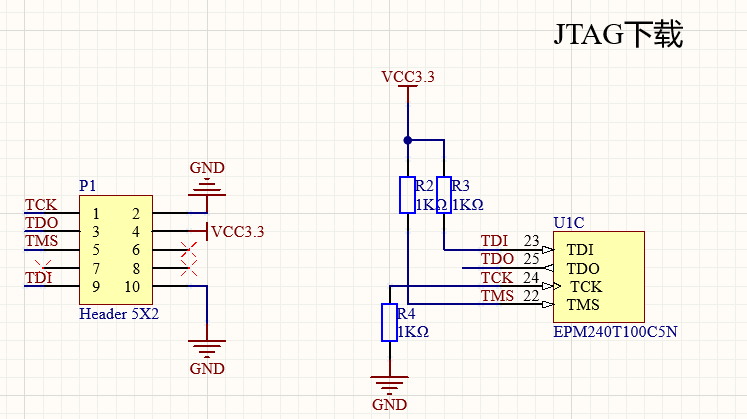
\includegraphics[width=7cm]{figure/JTAG download circuit.png}
        \caption{JTAG下载模块电路图}
        \label{JTAG下载模块电路图}
    \end{figure}
    
    \subsubsection{检测计数模块}
    检测计数模块的功能在于,亮灯提示钢化玻璃到位,并对经过的玻璃进行计数。如图\ref{检测计数模块电路图},CT引脚为MCU输出信号,当程序确定检测到物体后,CT引脚电压拉高,LED灯亮,当物体离开检测范围后,LED等灯灭。CT1引脚则是作为MCU的输入信号,当检测到一次物体后,CT1发出一次脉冲信号,计数加一,以此来实现计数功能。
    \begin{figure}[ht]
        \centering
        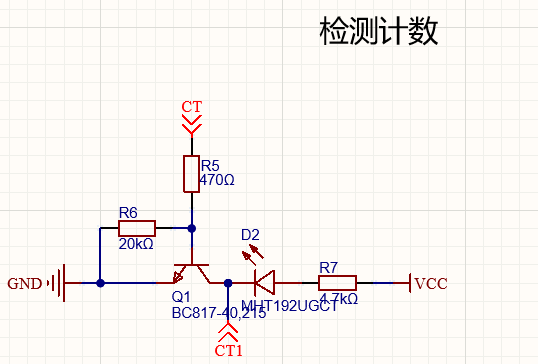
\includegraphics[width=7cm]{figure/detection count circuit.png}
        \caption{检测计数模块电路图}
        \label{检测计数模块电路图}
    \end{figure}
\newpage
       \subsubsection{超声波接近传感器控制电路PCB设计}
       在完成控制电路原理图的设计后,就将进行PCB部分的设计。如图\ref{超声波接近传感器整体PCB设计}为传感器PCB整体设计图,图\ref{超声波接近传感器控制电路PCB设计}为控制电路PCB的设计。
\begin{figure}[ht]
	\centering
	\subfloat[超声波接近传感器整体PCB设计]{
		\begin{minipage}[b]{0.5\textwidth}
			\centering
			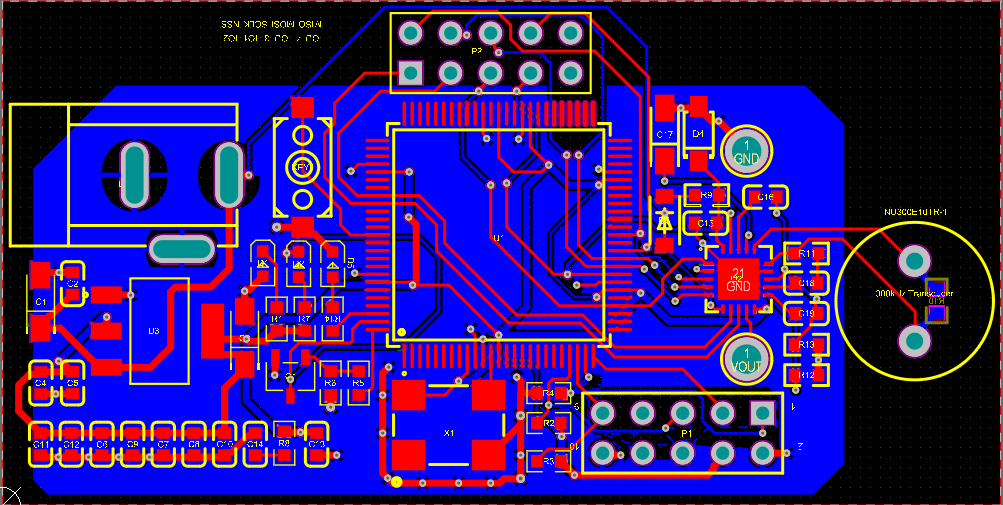
\includegraphics[height=4.5cm]{figure/overall pcb.png}
		\end{minipage}
		\label{超声波接近传感器整体PCB设计}
	}
	\subfloat[超声波接近传感器控制电路PCB设计]{
		\begin{minipage}[b]{0.5\textwidth}
			\centering
			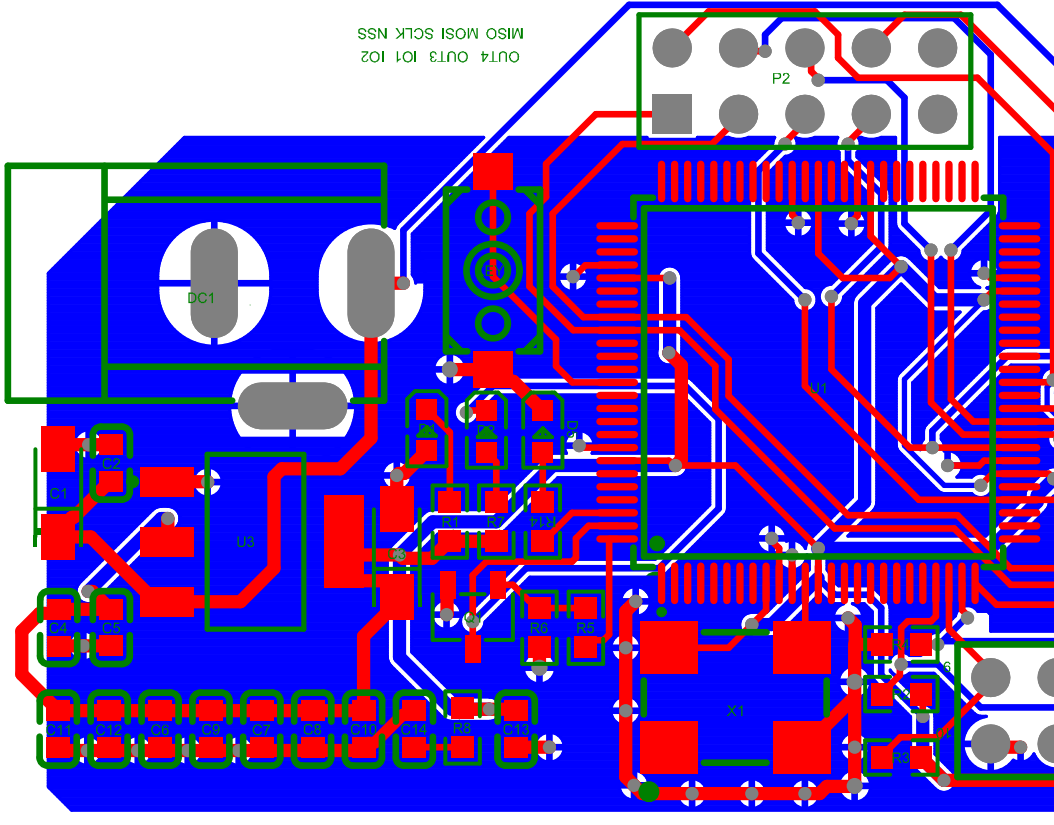
\includegraphics[height=4.5cm]{figure/cpld pcb.png}
		\end{minipage}
		\label{超声波接近传感器控制电路PCB设计}
	}
	\caption{超声波接近传感器PCB设计}
	\label{超声波接近传感器PCB设计}
\end{figure}
   \paragraph{线宽}
   对于功率较大的部分如电源、超声换能器驱动部分,需要对布线进行加宽处理,避免因发热而影响电路板正常工作,甚至产生损坏。\par
   \paragraph{时钟包地处理}
   对于速率较低的时钟,需进行包地处理。包地的作用主要有两点:一是拉开与其他信号的距离,从而减小干扰;二作为自身参考和屏蔽。包地处理还需要在地线上等间距打过孔。
  
 	\newpage
    \subsection{TUSS4470芯片外围电路}
    
    
    \begin{figure}[ht]
		\centering
		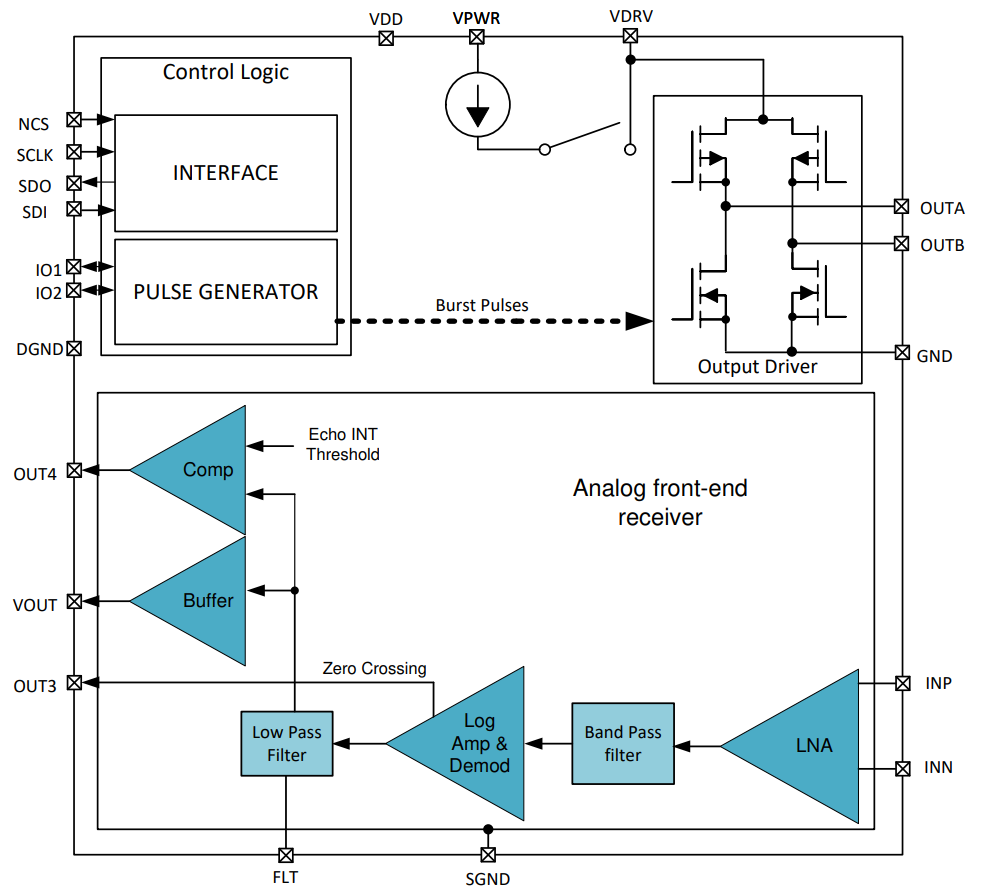
\includegraphics[width=12cm]{figure/Function Block Diagram.png}
		\caption{TUSS4470芯片功能框图}
		\label{TUSS4470芯片功能框图}%文中引用该图片代号
\end{figure}
 图\ref{TUSS4470芯片功能框图}为TUSS4470驱动芯片的整体功能框图\upcite{TUSS4470芯片手册},以此作为外围电路设计的参考资料。如图所示,芯片按照功能可分为逻辑控制、输出驱动、回波接收三个部分。其中逻辑控制部分又分为SPI通信和脉冲发生模块,SPI通信模块用于接收MCU芯片发送的芯片配置数据,脉冲发生模块的两个引脚IO1、IO2连接MCU芯片作为脉冲发生控制引脚,根据芯片不同的IO模式,两个引脚配合产生指定脉宽、脉冲数的脉冲信号;输出驱动模块的OUTA、OUTB引脚直接连接超声换能器,VDRV引脚连接外部电容,VPWR可对电容充电,在VDRV到达设定电压值后,VPWR停止对VDRV供电,这使得超声换能器的驱动电压可以保持在设定值,以此保证发出脉冲的声压水平可以稳定在一定水平,从而保证发射出稳定的脉冲波(其中VDRV的设定电压可通过SPI对芯片进行配置);回波接收模块的作用在于:对回波信号进行处理,输出可供MCU进行检测判断的信号其中INP、INN引脚连接超声波换能器的正负端,FLT连接外部电容作为低通滤波器对回波信号进行滤波处理。OUT3引脚内部连接至模块中的对数解调模块,当回波信号在模块内进完成放大进行解调时,将某阶段信号作为零点,输出过零信号,以验证接收信号的频率, 提高对其他信号的抗干扰性。OUT4作为检测到位的指示信号,当VOUT输出电压超过芯片配置数据中设定的阈值时,OUT4拉高。(VOUT引脚的电压值由公式\ref{VOUT公式}决定)。
  
    \begin{equation}
        V_{OUT}=G_{VOUT} \cdot SL_{LOG}\cdot20log_{10}(\frac{G_{LNA} \cdot G_{BPF} \cdot V_{IN}}{INT_{LOG} \cdot K_X})
        \label{VOUT公式}
    \end{equation}
式中\quad $G_{VOUT}$---对数放大器斜率增益调整(Slope or gain adjustment);\par
\quad$SL_{LOG}$---对数运算放大器斜率调整(slope of logarithmicamplifier);\par
\quad$G_{LNA}$---回波增益;\par
\quad$G_{BPF}$---$0.9v/v$;\par
\quad$V_{IN}$---INN引脚输入;\par
\quad$INT_{LOG}$---对数放大器截距( logarithmic amplifier intercept);\par
\quad$K_X$---对数截距平差(log intercept adjustment)\par
    回波接收模块的详细工作框图如图\ref{回波接收模块}所示。
    \begin{figure}[ht]
        \centering
        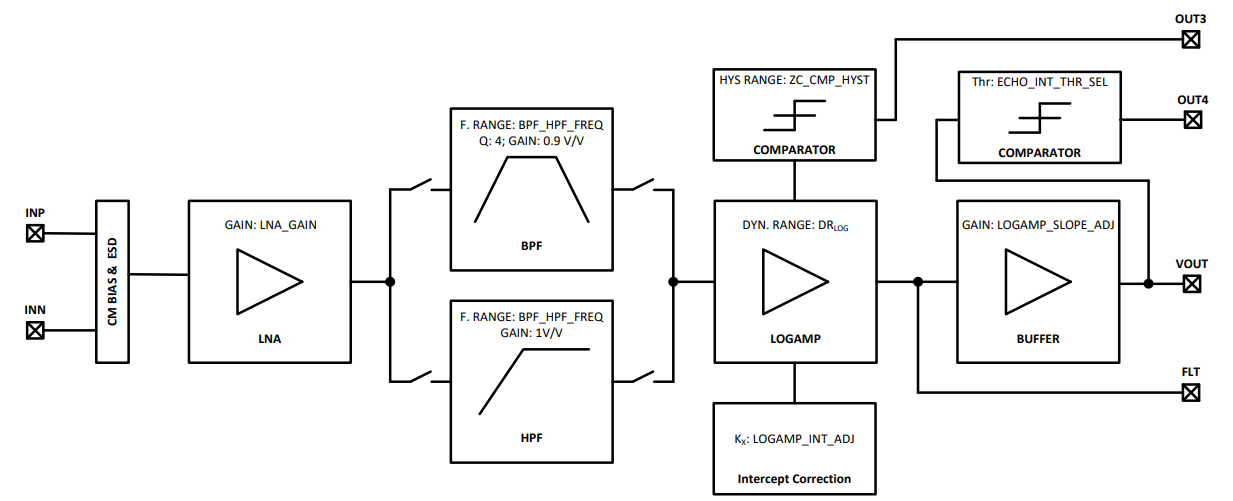
\includegraphics[width=10cm]{figure/Analog Front-End Block Diagram.png}
        \caption{回波接收模块}
        \label{回波接收模块}
    \end{figure}\par

    参考芯片手册相关内容,进行了TUSS4470芯片外围电路的设计,如图\ref{TUSS4470芯片外围电路}所示。
    \begin{figure}[!h]
        \centering
        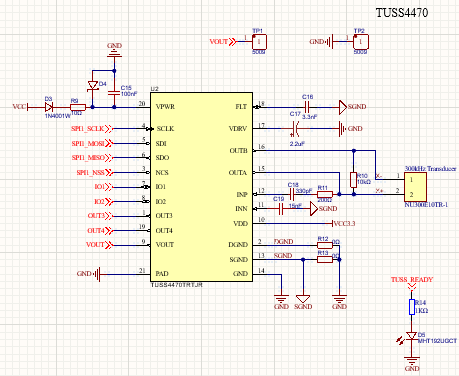
\includegraphics[width=9cm]{figure/TUSS4470 peripheral circuit.png}
        \caption{TUSS4470芯片外围电路}
        \label{TUSS4470芯片外围电路}
    \end{figure}
\newpage
    \subsubsection{VPWR引脚电路}
    VPWR引脚输入电压范围为5V到36V,TUSS4470设备可能受到电池瞬变和反向电流的影响,因此采用外部组件保护芯片十分必要。图\ref{VPWR引脚}中除了靠近引脚的电容C15,二极管D3、D4和电阻R9就起到了保护芯片的作用。
     \begin{figure}[ht]
    	\centering
    	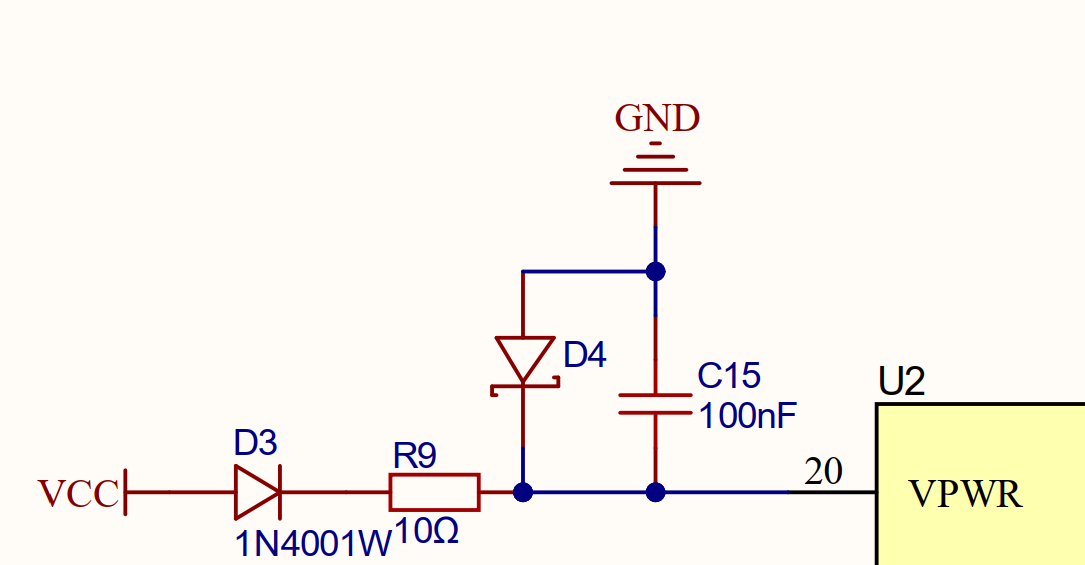
\includegraphics[width=10cm]{figure/VPWR PIN.png}
    	\caption{VPWR引脚电路}
    	\label{VPWR引脚}
    \end{figure}
        \subsubsection{FLT外接滤波电容}
    FLT引脚外接滤波电容,对应图\ref{TUSS4470芯片功能框图}回波检测模块中的低通滤波器。该滤波电容的作用在于,去除对数放大器输出中的高频信号,使解调包络信号有足够的峰值保持时间,而截止频率的大小则由FLT引脚的阻抗以及外接电容的电容量所决定,该电容虽然可以抑制高频信号的波动,但同样会减缓信号的响应速度。大电容量可以使VOUT引脚输出的电压峰值变化减小,并且减缓上升下降到峰值的时间,而最优电容量则需在应用中不断进行优化。本设计初步使用电容量为3.3nF的电容。
    \subsubsection{VDRV引脚电路}    
    VDRV引脚连接外部电容,TUSS4470芯片通过VPWR引脚为外部的电容充电,当其达到设定电压时则停止充电,此时该电容将为超声换能器H桥驱动电路供能。
     \subsubsection{超声换能器驱动电路}
    在TUSS4470的芯片手册中,超声换能器有四种不同的驱动方式,不同驱动方式产生脉冲的方式也不同,本设计中采用最典型的HALF\_BRG\_MODE\_0来进行驱动,如图\ref{参考配置方式}为参考配置方式,图\ref{实际配置方式}为本设计中所采用的方式。
    
\begin{figure}[ht]
	\centering
	\subfloat[参考配置方式]{
		\begin{minipage}[b]{0.5\textwidth}
			\centering
			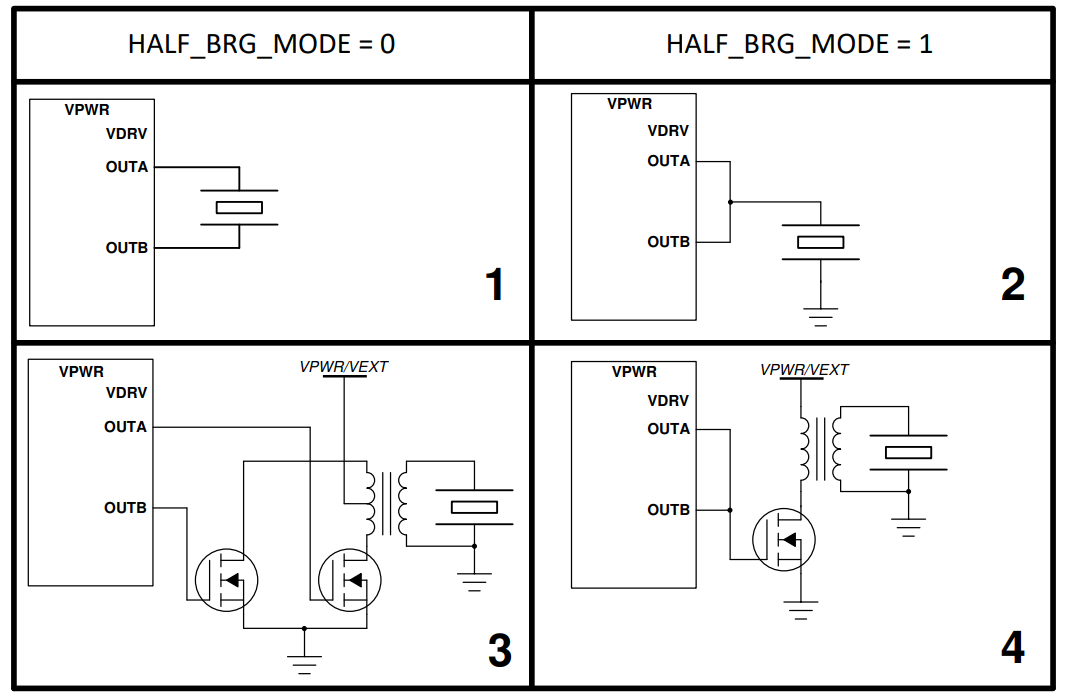
\includegraphics[height=4.5cm]{figure/TUSS4470 Transducer Drive Options.png}
		\end{minipage}
		\label{参考配置方式}
	}
	\subfloat[实际配置方式]{
		\begin{minipage}[b]{0.5\textwidth}
			\centering
			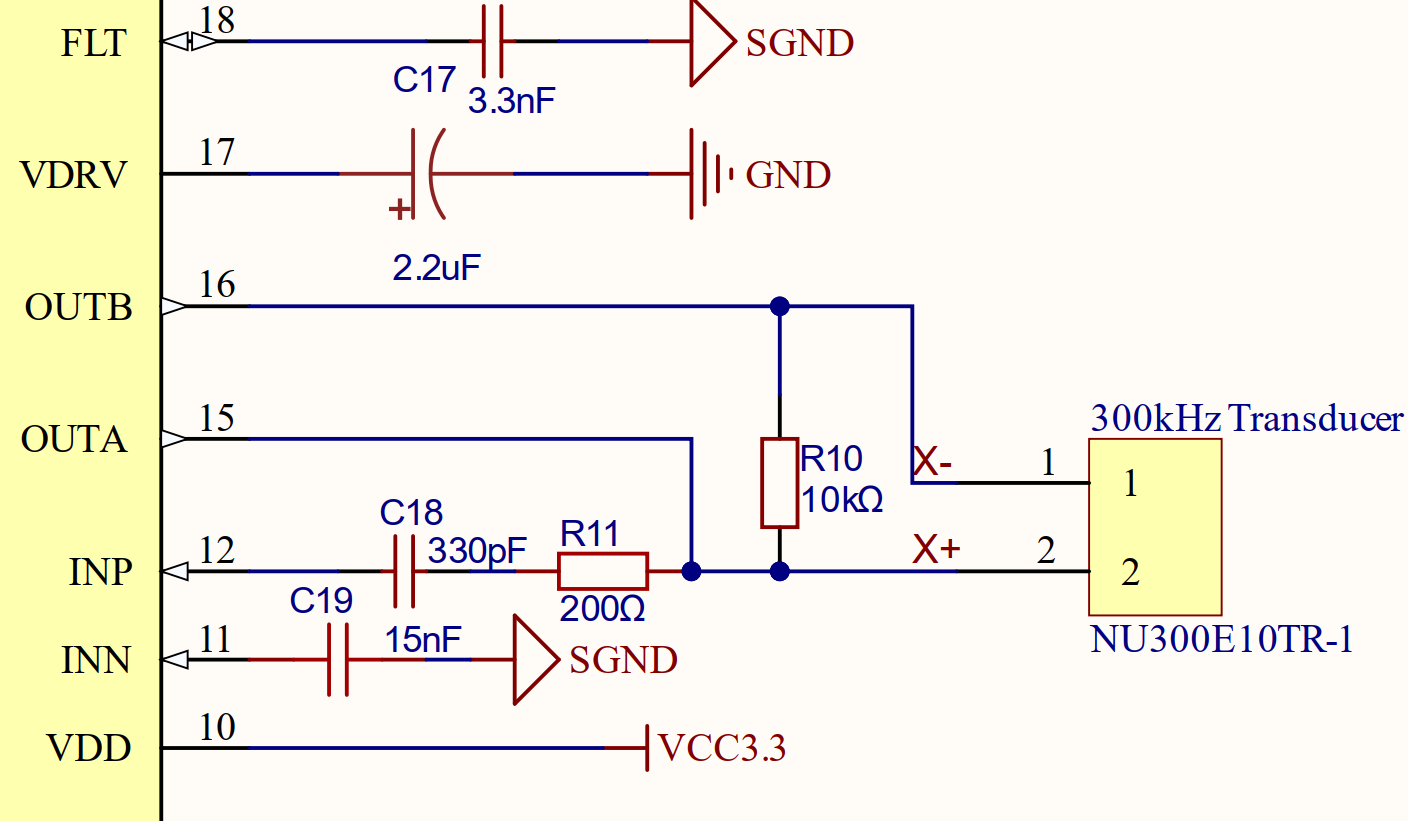
\includegraphics[height=4.5cm]{figure/OUTA PIN.png}
		\end{minipage}
		\label{实际配置方式}
	}
	\caption{超声换能器驱动电路设计}
	\label{超声换能器驱动电路设计}
\end{figure}
    \subsubsection{芯片配置指示电路}
    CPLD芯片通过SPI协议向TUSS4470芯片发送配置数据,并接收其反馈回数据。在芯片返回的数据当中,有一位的状态位用来反映芯片是否准备就绪,当芯片准备就绪后该位置1,可供MCU进行下一步的工作。如图为芯片配置指示电路,当芯片配置就绪后,MCU该引脚拉高,LED灯亮,用来指示芯片的配置状态。
    \subsubsection{分离接地电路}
    由于外围电路中包含多种类型的信号,例如VPWR引脚的电源信号,VOUT引脚的模拟信号,VOUT引脚的模拟信号,SCLK等引脚的数字信号。当产生数字信号的引脚产生脉冲时,其变换速度较快,将会在数字地产生较大的噪声;而模拟信号又容易受到外接的干扰,如果将数字信号和模拟信号直接接入同一个大地,将会严重影响模拟信号的准确性,对于超声波传感器而言,是非常致命的。本设计在原理图设计的过程中便解决了不同类型分离接地\upcite{分离接地}的问题,采用的方法是:先将不同类型的信号连接到0$\Omega$电阻,再连接到大地,0$\Omega$电阻相当于很窄的电容通道,能够有效的限制环路电流,使噪声得到抑制。起分离接地作用的电路如\ref{分离接地电路}所示。
     \begin{figure}[!h]
        \centering
        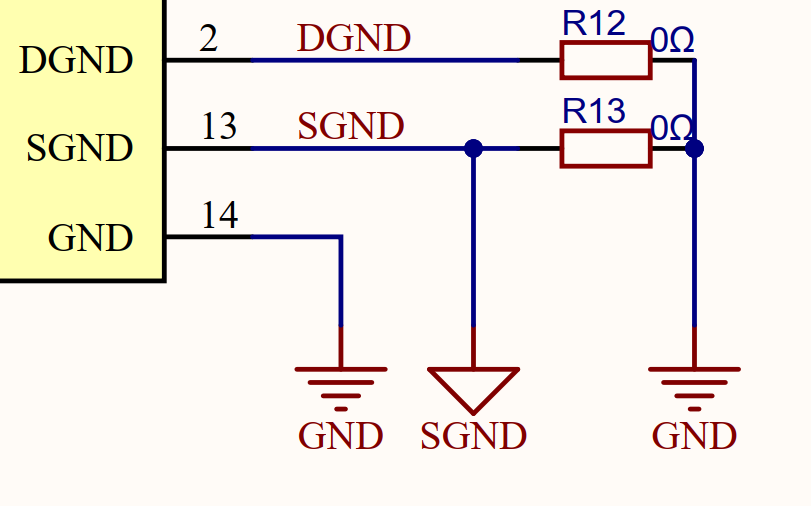
\includegraphics[width=7cm]{figure/seperate ground.png}
        \caption{分离接地电路}
        \label{分离接地电路}
    \end{figure}
	\subsubsection{TUSS4479芯片外围电路PCB设计}
    由于本设计中涉及到的信号类型较多,包括了数字信号、模拟信号、高频信号、大功率信号,各信号间会存在较大的干扰,因此在布线过程中将各信号分离十分重要,直接关系到传感器的稳定性和精度。如图\ref{TUSS4470芯片外围电路PCB设计}为TUSS4470芯片外围电路PCB设计,图\ref{TUSS4470芯片引脚图}为芯片对应的引脚图。本设计采用两层板来完成布线。
  \begin{figure}[!h]
   		\begin{minipage}[t]{0.5\linewidth}
  			\centering
  			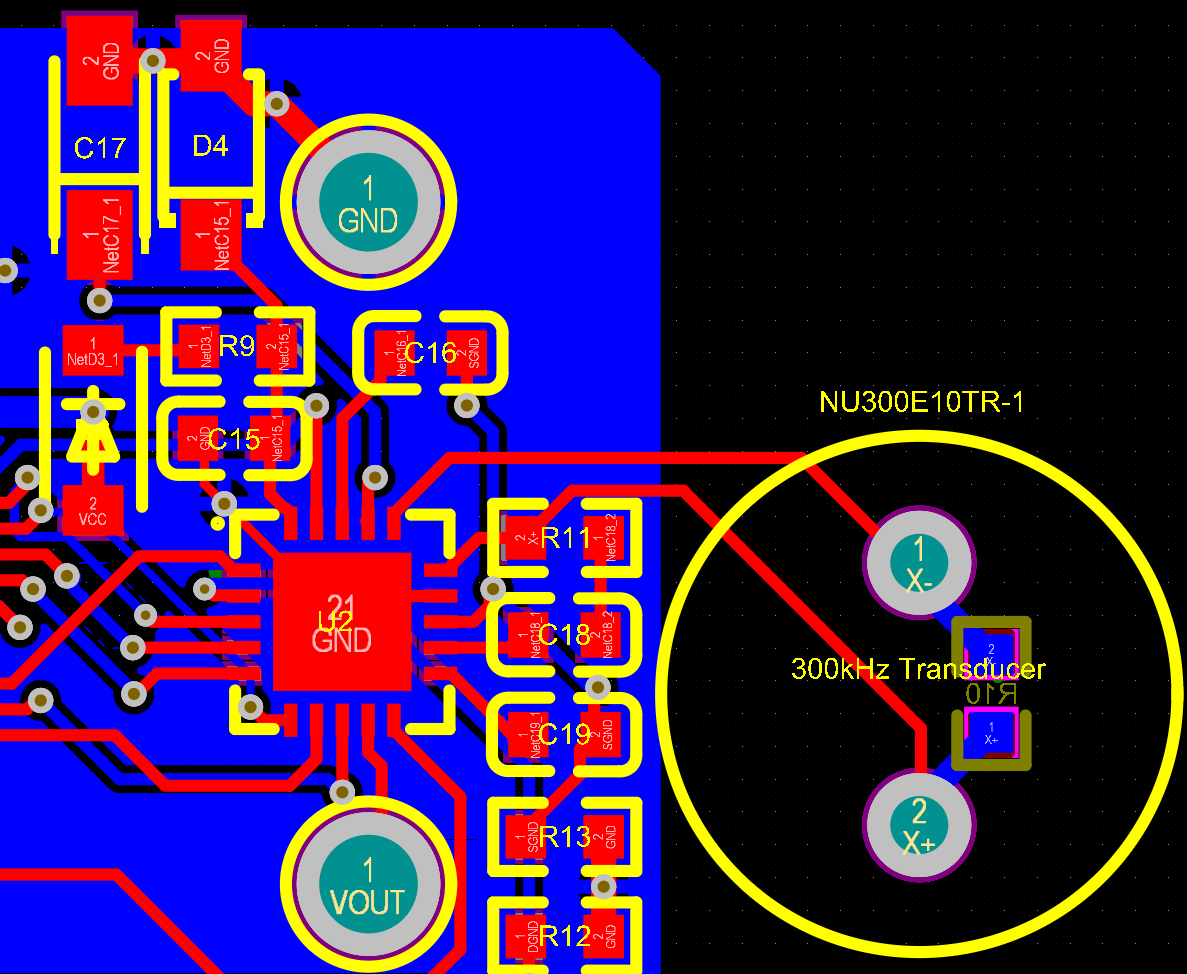
\includegraphics[height=5cm]{figure/TUSS4470 pcb.png}
  			\caption{TUSS4470芯片外围电路PCB设计}
  			\label{TUSS4470芯片外围电路PCB设计}
  		\end{minipage}
   		\begin{minipage}[t]{0.5\linewidth}
  			\centering
  			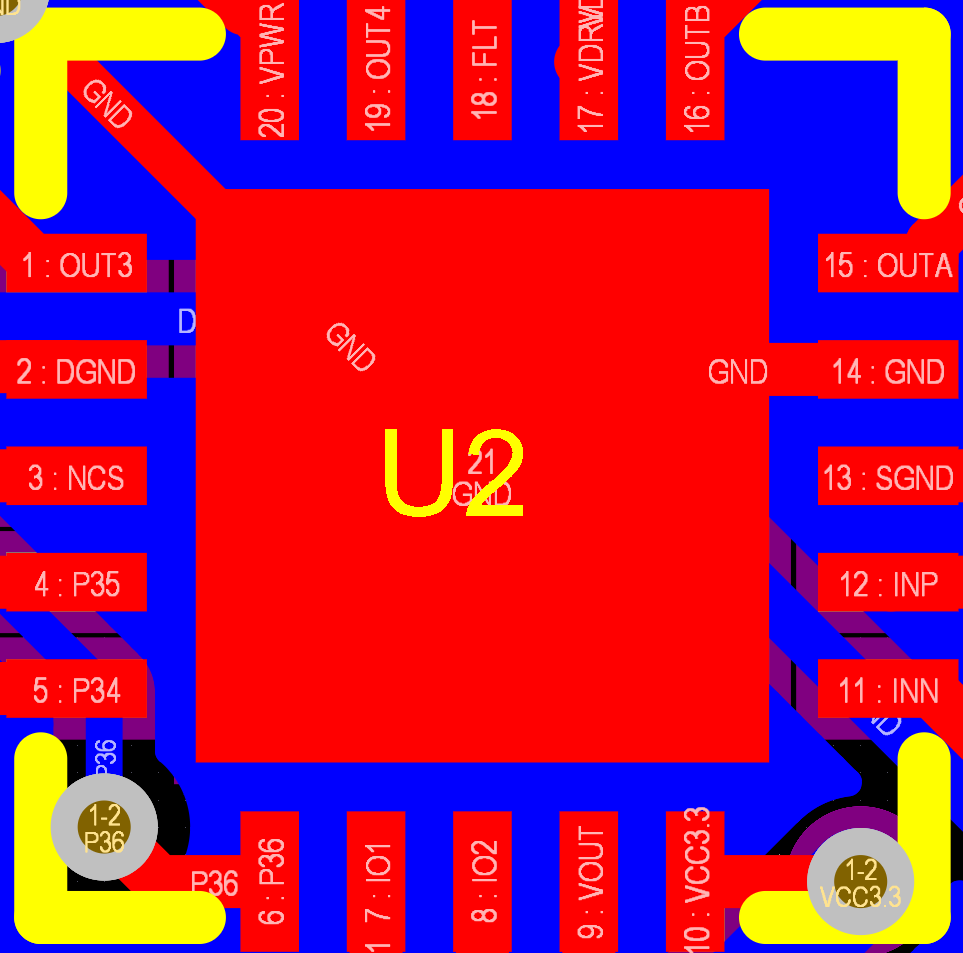
\includegraphics[height=5cm]{figure/TUSS4470 PIN.png}
  			\caption{TUSS4470芯片引脚图}
  			\label{TUSS4470芯片引脚图}
  		\end{minipage}  		 
  \end{figure}\par
    在TUSS4470驱动芯片的PCB设计过程中,最重要的就是将芯片的电源信号、数字信号以及模拟信号进行分离。参考芯片手册\upcite{TUSS4470芯片手册},在布线时考虑到了如下事项。\par
    \paragraph{各类信号分离接地}
    在连接到主地前,数字接地、传感器接地、回波接地都要先通过0$\Omega$电阻或者铜迹线,如图\ref{分离接地电路},本设计在原理图设计时采用了0$\Omega$电阻的方式来实现分离接地,因此在布线时就不需要考虑该问题。
     \paragraph{回波接收引脚}
    INN、INP引脚作为回波信号的接收引脚,对噪声干扰十分敏感,所以其布线必须要短且直,并且保证INN引脚的电容尽量靠近芯片引脚,以减少干扰,但考虑到后续需手工焊接,电容与芯片引脚间仍要保持一定的间隙,以减小手工焊接的难度。假设不考虑测试成本,采用贴片工艺,电容与芯片引脚间的距离还可再进一步减小,以获得到具有更高稳定性的回波信号。
    \paragraph{VOUT引脚}
    VOUT引脚作为模拟信号输出端,与外界的连线应该尽量短直,避免产生寄生效应\upcite{寄生效应},以及外部噪声干扰引起的噪声耦合。\par
    \paragraph{超声换能器驱动}
    芯片与OUTA、OUTB引脚间的布线应尽可能短且直,以保证发出脉冲信号的质量,从而提高传感器的精度。考虑到两个引脚输出的是大功率、高频率的模拟信号,连接到两引脚的线宽应不能太小。\par
    \paragraph{VPWR引脚}
        根据芯片手册推荐,VPWR的解调电容应尽可能靠近引脚。\par
     \paragraph{信号分离}
     数字信号引脚如TXD、RXD、 SCLK、 NCS、IO1、 IO2、 OUT3、OUT4应远离模拟信号引脚,避免信号间的干扰。\par
\subsection{本章小结}
本章主要介绍了超声波接近传感器硬件部分的设计,首先介绍了超声波接近传感器控制电路的设计,该部分包括了原理图设计和PCB设计,重点讲解了JTAG下载模块的设计和时钟包地处理。然后又详细介绍了TUSS4470芯片外围电路的设计,该部分讲解了各管脚连接器件的选型以及PCB设计过程中需要注意的事项,原理图设计部分详细介绍了VPWR引脚、VDRV引脚以及各类信号分离接地处理的设计,而PCB设计部分则详细介绍了各类器件的布局原则,以减少信号间的相互干扰。\par
至此已介绍完成了超声波接近传感器原理图设计和PCB设计部分的工作,下一章将详细讲解传感器的软件设计部分。

      
    
    
    
 %------------------第四章---------------------------
    \newpage
	\section{传感器程序设计}
    \subsection{传感器检测原理与检测策略}
    

    
    \subsubsection{检测原理}
    超声波一般指振动频率超过20KHz的脉冲波,其具有频率高、波长锻、穿透性强以及绕射性小等特点\upcite{检测原理},当遇到杂质或材料分界面时,会产生显著的反射效应形成回波利用回波信号可进行距离检测、表面缺陷排查、材质判断等方面的应用,而本设计中超声波传感器则用于生产线钢化玻璃的接近检测。
    超声波信号的振幅会随其传播距离的增大而不断减小,通过滤波解调等处理,可将回波信号处理成一个简单的单峰信号,如公式\ref{VOUT公式}以及图\ref{回波接收模块}所示,将不同距离的回波进行处理,可以得到不同峰值的单峰信号,通过检测峰值来判断物体是否到达指定位置。
    如图\ref{VOUT输出},为20V驱动电压下, LNA\_GAIN = 0x0; VOUT\_SCALE\_SEL = 0x0; 
LOGAMP\_DIS\_FIRST = 0x0; LOGAMP\_DIS\_LAST = 0x0时不同距离对应VOUT的输出,可以看到,随着检测距离的减小,VOUT输出的峰值也在不断减小。\par
    \begin{figure}[H]
        \centering
        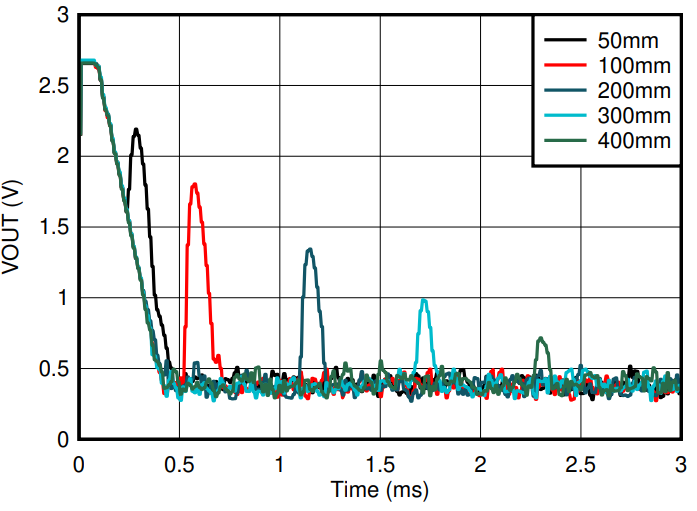
\includegraphics[width=10cm]{figure/VOUT image.png}
        \caption{VOUT输出}
        \label{VOUT输出}
    \end{figure}
    在应用中,首先通过SPI接口向ECHO\_INT\_CONFIG寄存器配置VOUT引脚的阈值,当引脚的电压超过所配置的阈值时,即判断为检测到了物体,OUT4引脚拉高,将其作为控制信号连接至MCU。\par
    TUSS4470驱动芯片还提供了过零检测的功能,通过OUT3引脚输出的过零信号,可对回波频率进行再次检测,增加对其它信号的抗干扰性。该过零信号来自图\ref{TUSS4470芯片功能框图}
    中的对数模块,当信号在其中进行解调时,可根据应用选取特定阶段的信号作为零点。该过零信号仅在OUT4拉高时才有输出,以避免其它噪声的干扰。
    \subsubsection{检测策略}
      在配置完成TUSS4470驱动芯片后,即可开始产生脉冲信号并通过超声换能器发送脉冲波。与传统的超声波传感器不同,采用该驱动芯片可发送指定次数、指定脉冲数的脉冲波,这就为我们设计丰富的检测策略提供了硬件基础。考虑到钢化玻璃处于复杂的工厂环境,传感器易受到各种电磁信号的影响,因此增加传感器的稳定性就变得至关重要。\par
      本设计采用多次发射脉冲波的检测策略,在发送完一次指定脉冲数的脉冲波之后,传感器就进入检测模式,假如检测到了有效回波,检测标志位加一。连续发射五次脉冲,以五次脉冲波的发射作为一次检测周期,每个检测周期后都会更新检测状态。当一个检测周期内有超过三次检测到有效回波时,判断为检测到物体,DETECTED\_STATE=1,LED灯亮;有效脉冲波的次数小于或等于三次时,判断为未检测到物体,DETECTED\_STATE=0,\par\noindent LED灯灭。如图\ref{检测逻辑流程图}为实现检测逻辑的程序流程图,图\ref{检测状态转移图}为检测状态转移图。
     \begin{figure}[H]
      \begin{minipage}{0.5\linewidth}
		\centering
		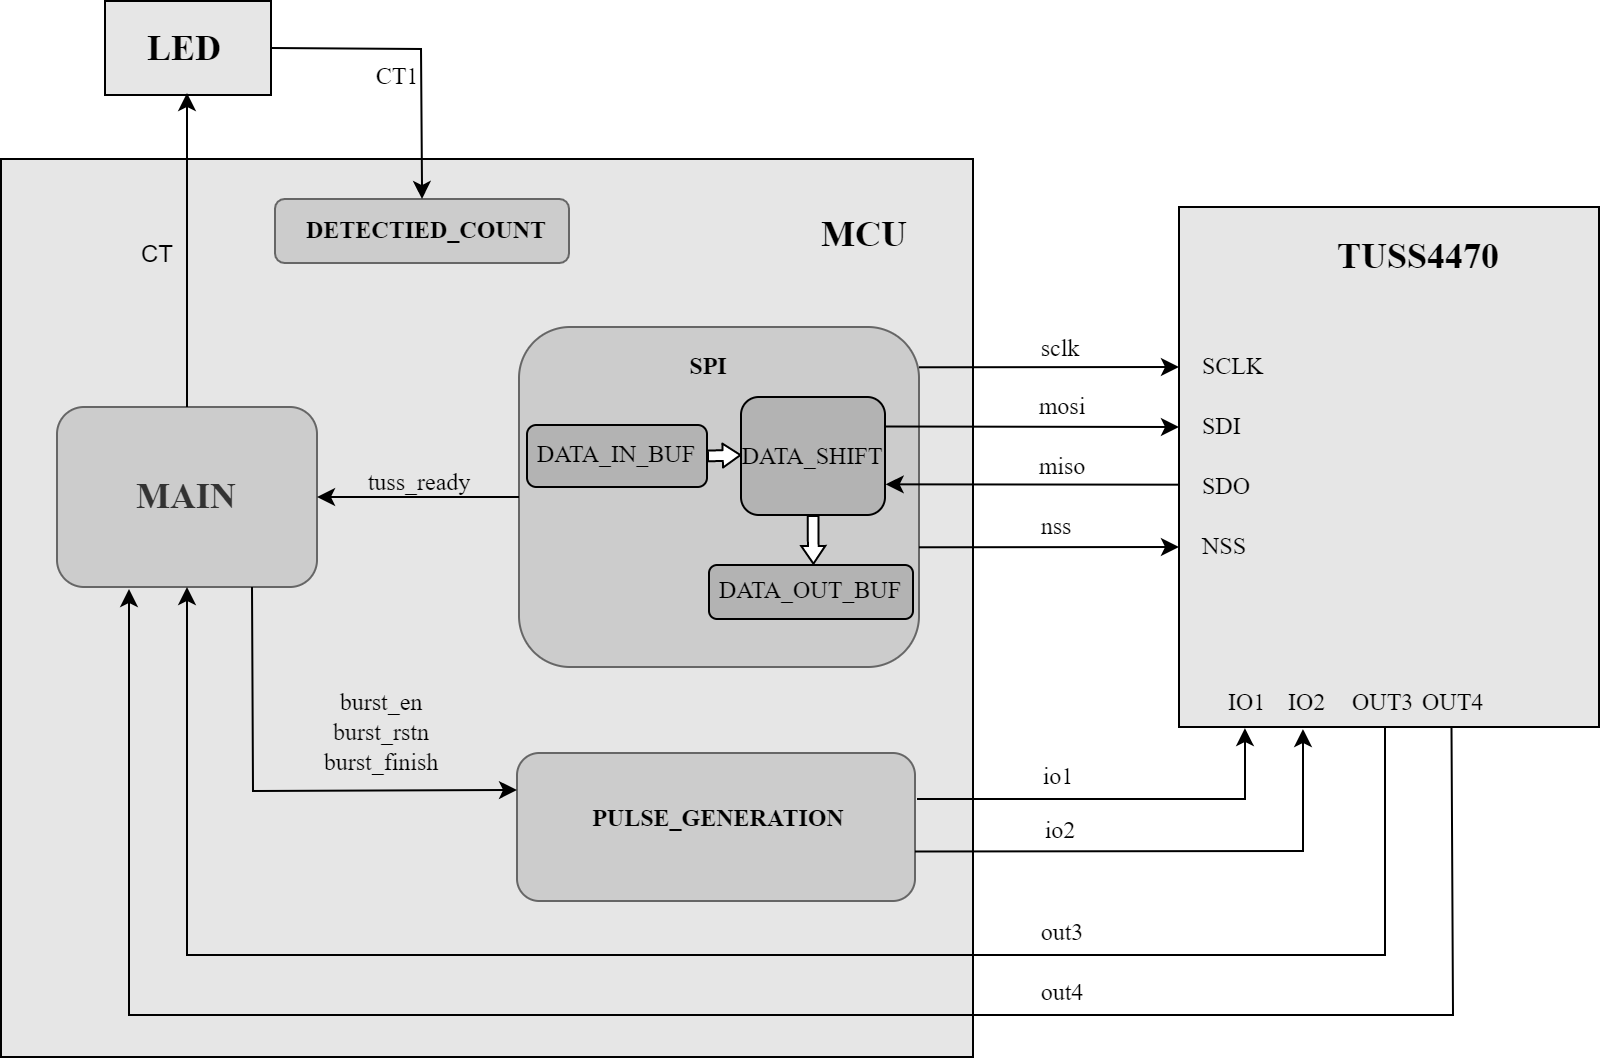
\includegraphics[width=5cm]{figure/Overall program block diagram.png}
		\caption{检测逻辑流程图}
		\label{检测逻辑流程图}%文中引用该图片代号
	\end{minipage}
	%\qquad
	\begin{minipage}{0.4\linewidth}
		\centering
		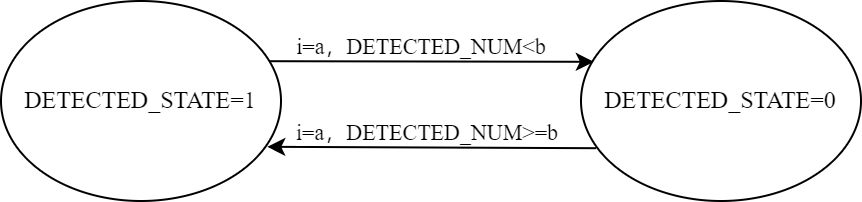
\includegraphics[width=5cm]{figure/LED state transition diagram.png}
		\caption{检测状态转移图}
		\label{检测状态转移图}%文中引用该图片代号
	\end{minipage}
\end{figure}
    此种检测策略可以极大的增加传感器的稳定性,只有在指定位置持续检测到钢化玻璃时才会认为检测到物体,一定程度上可以避免发生因外界干扰而出现错误检测的情况。
    
      
      
  
      
    
    \subsection{传感器程序设计,解释代码}
    \subsubsection{程序总体设计}
    本设计所使用的EPM240T100C5N芯片采用Verilog HDL作为编程语言,Quartus II作为编程烧录软件。Verilog HDL\upcite{Verilog介绍}是一种硬件描述语言(HDL:Hardware Description Language),以文本形式来描述数字系统硬件的结构和行为的语言,用它可以表示逻辑电路图、逻辑表达式,还可以表示数字逻辑系统所完成的逻辑功能。\par
    在本设计中,如图\ref{程序整体框图}所示,将MCU分成四个模块,分别是:MAIN模块、SPI模块、PULSE\_GENERATION模块、DETECTED\_COUNT模块,实现配置TUSS4470芯片、产生脉冲信号、到位指示以及计数等功能。
    
         \begin{figure}[H]
        \centering
        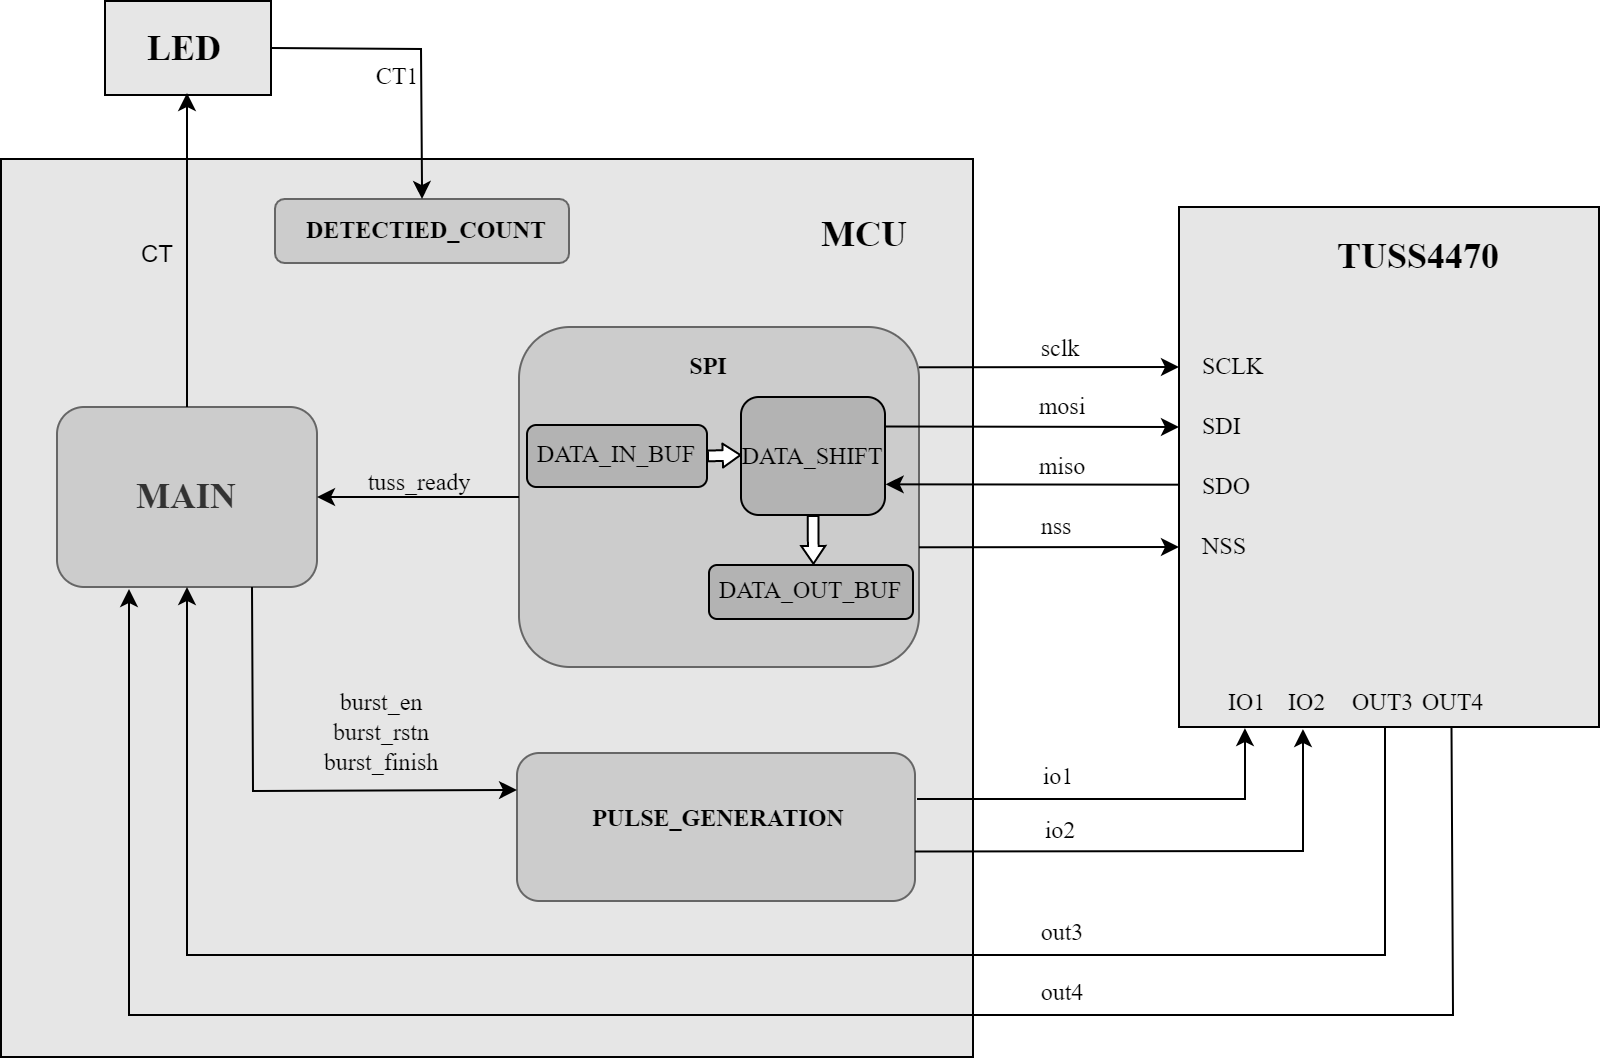
\includegraphics[width=12cm]{figure/Overall program block diagram.png}
        \songti\zihao{5}\caption{程序整体框图}
        \label{程序整体框图}
    \end{figure}
    
    \subsubsection{控制模块}
    图\ref{程序整体框图}中的MAIN模块为传感器的控制模块,其作用在于,协调各模块间的工作,是程序的主要部分,图\ref{MAIN模块程序流程图}为MAIN模块的工作流程图。
    首先是SPI模块向TUSS4470芯片发送配置数据,并接收从TUSS4470反馈回的芯片状态;根据反馈数据判断芯片是否准备就绪,当准备就绪后向MAIN模块发送tuss\_ready信号;之后通过IO1、IO2引脚配合控制产生脉冲信号,在每次发送完脉冲信号后,都会根据OUT3、OUT4引脚返回的信息判断本次是否检测到物体;多次检测到预定回波后即确认为检测到物体,通过CT引脚控制LED灯亮;检测计数模块也将进行计数。
    \begin{figure}[H]
        \centering
        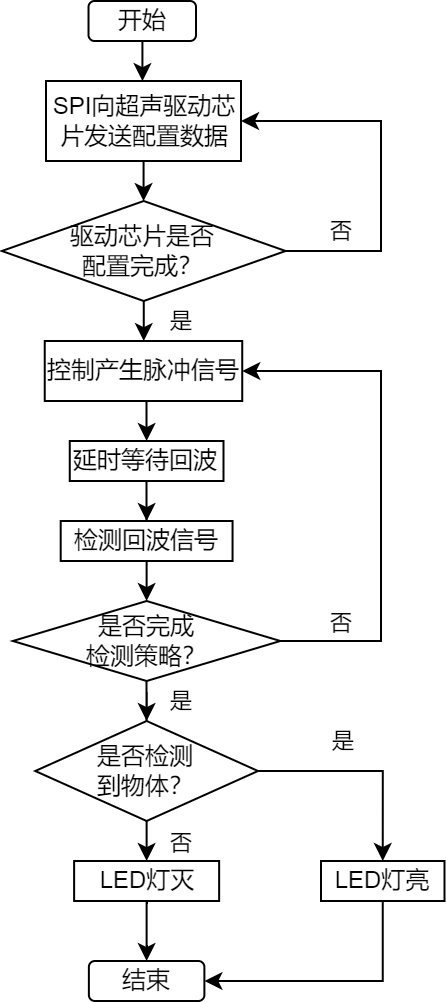
\includegraphics[width=5cm]{figure/MAIN module flow chart.png}
        \songti\zihao{5}\caption{MAIN模块程序流程图}
        \label{MAIN模块程序流程图}
    \end{figure}
    
    
    
    \subsubsection{SPI通信模块}
    \noindent
    \textbf{1、介绍}\par
    在本设计中,MCU芯片通过SPI通信协议来配置TUSS4470芯片。SPI\upcite{SPI}是串行外设接口(Serial Peripheral Interface)的缩写,是Motorola公司推出的一种同步串行接口技术,是一种高速、全双工、同步的通信总线。\par
    在本设计中,采用的是四线制SPI,其包括:SCLK(时钟信号)、NCS(片选信号)、MOSI(MCU输出信号)、MISO(MCU输入信号)。SCLK时钟信号和NCS片选信号都由主设备产生,NCS信号拉低为有效信号。
    
    \noindent
    \textbf{2、模式选择}\par
    SPI通信模式通过CPOL(时钟极性)和CPHA(时钟相位)来确定。其中CPOL配置SCLK电平的有效态,当CPOL=0时,SCLK低电平处于空闲态,高电平有效,当CPOL=1时,SCLK高电平为空闲态,低电平有效;CPHA配置数据采样发生在第几个边沿,当CPHA=0时,在第一个边沿数据采样,在第二个边沿数据发送,当CPHA=1时,在第一个边沿数据发送,在第二个边沿数据采样。\par
    根据芯片手册可以得知驱动芯片为高电平有效,在上升沿接收数据,在下降沿发送数据,即MCU在上升沿发送数据,在下降沿接收数据,可以得知选择的SPI模式为:CPOL=0,CPHA=1。
    
    \noindent
    \textbf{3、实现原理}\par
    SPI的全双工通信通过一个移位寄存器DATA\_SHIFT来实现。待发送的数据首先写入DATA\_IN\_BUF中进行缓存,需要发送时写入DATA\_SHIFT中,通过移位先将高位数据发送给从机,再将接收到的数据存储到低位,以8位的移位寄存器为例,其工作示意图如图\ref{移位寄存器工作示意图}所示,当发送完成8位数据11110000时,也完成了数据的接收。在接收完成数据后,将数据存入到DATA\_OUT\_BUF寄存器中,至此实现了一帧数据的收发流程。
        \begin{figure}[H]
        \centering
        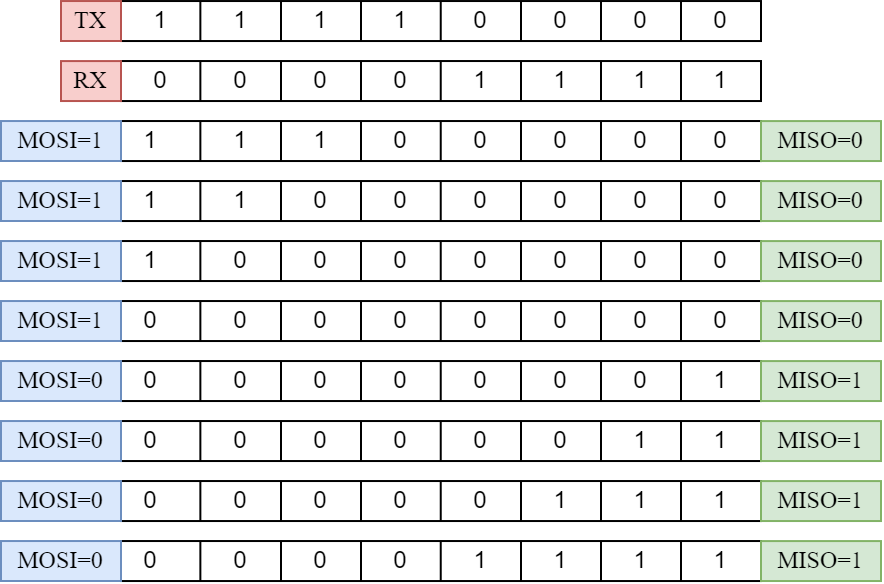
\includegraphics[width=10cm]{figure/DATA_SHIFT.png}
        \songti\zihao{5}\caption{移位寄存器工作示意图}
        \label{移位寄存器工作示意图}
    \end{figure}
    
    
    \noindent
    \textbf{4、程序设计}\par
    单帧数据的发送采用线性序列机的方式来实现,即利用一个计数器不断计数,计数器的每一个值都对应一个时刻,在不同时刻对DATA\_SHIFT寄存器采取不同操作,如表\ref{线性序列机}所示。当复位时,对DATA\_SHIFT寄存器进行初始化;当计数器CNT为0时,将DATA\_IN\_BUF内的数据赋值给DATA\_SHIFT;当CNT为1-16时,DATA\_SHIFT寄存器进行移位操作;当CNT=17时,将DATA\_SHIFT内的数据赋值给DATA\_OUT\_BUF,至此单帧数据收发完毕,在这基础上,将进行多帧数据的收发。
    
    \begin{table}[H]
        \centering
        \caption{线性序列机}
    \begin{tabular}{c|c}
    \hline
    CNT & 操作  \\ \hline
    复位 & \begin{lstlisting}
        DATA_SHIFT=0;DATA_OUT_BUF=0;
            \end{lstlisting}    \\ \hline
    
    0 & \begin{lstlisting}
        DATA_SHIFT=DATA_IN_BUF;
        \end{lstlisting}   \\ \hline
    
    1-16&  \begin{lstlisting}
    mosi<=DATA_SHIFT[15];DATA_SHIFT<={DATA_SHIFT[14:0],miso};
            \end{lstlisting} \\ \hline
    
    17&     \begin{lstlisting}
        DATA_OUT_BUF<=DATA_SHIFT;
            \end{lstlisting}  \\ \hline
            
        \end{tabular}
                \label{线性序列机}
    \end{table}
    
    TUSS4470芯片采用高位先发的方式来收发数据,当NCS信号拉低时,SPI模块开始工作,当NCS拉高,SPI模块停止工作,完成一帧数据的收发。SPI无法实现连续收发多帧的数据,在每帧数据的收发之间NCS需要经历低-高-低的过程。实现多帧数据收发的程序流程图如图\ref{收发多帧数据程序流程图}所示,该程序可一次性发送9帧16位的数据至TUSS4470驱动芯片。
    \begin{figure}[H]
        \centering
        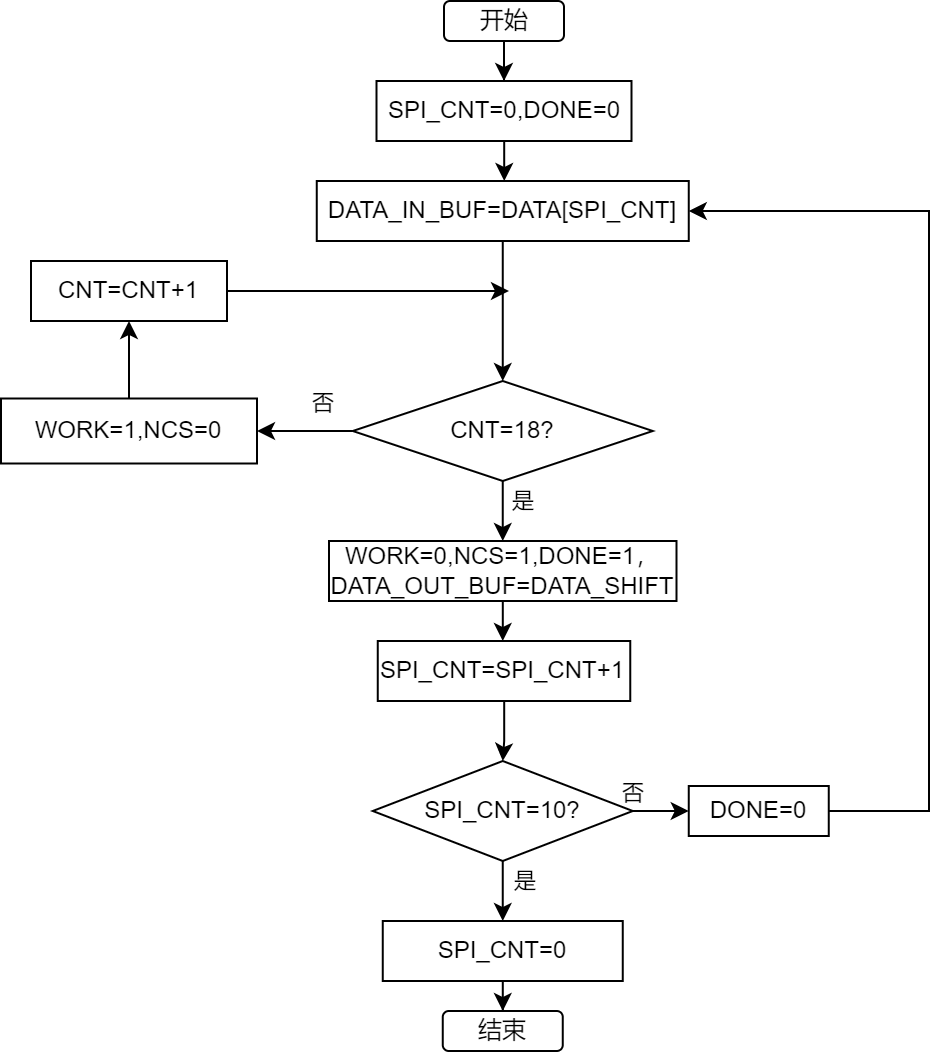
\includegraphics[width=10cm]{figure/SPI Program Flow Chart.png}
        \songti\zihao{5}\caption{收发多帧数据程序流程图}
        \label{收发多帧数据程序流程图}
    \end{figure} 
    图中SPI\_CNT用于记录收发数据的帧数;DONE为每帧数据发送完成标志位;WORK为工作位,用于记录工作状态;DATA为一个$10\times16$的数组,用于存放配置数据。
    程序开始运行后,首先进行数据初始化,然后将DATA寄存器内的数据赋给DATA\_IN\_BUF寄存器,片选信号NCS拉低,进行单帧数据的收发。当CNT=18时完成单帧数据的收发,DONE置1,片选信号NCS拉高,帧数计数位SPI\_CNT+1,DONE、CNT置零。在将DATA内的数据发送完成后,根据驱动芯片返回的数据判断芯片是否完成配置,如果完成配置,SPI通信模块将向main模块发送tuss\_ready信号,反之则重新进行配置。
    
    
    

    
    \noindent
    \textbf{5、数据结构}\par
    图\ref{SPI数据结构图1}为SPI通信的数据结构图
    \begin{figure}[H]
        \centering
        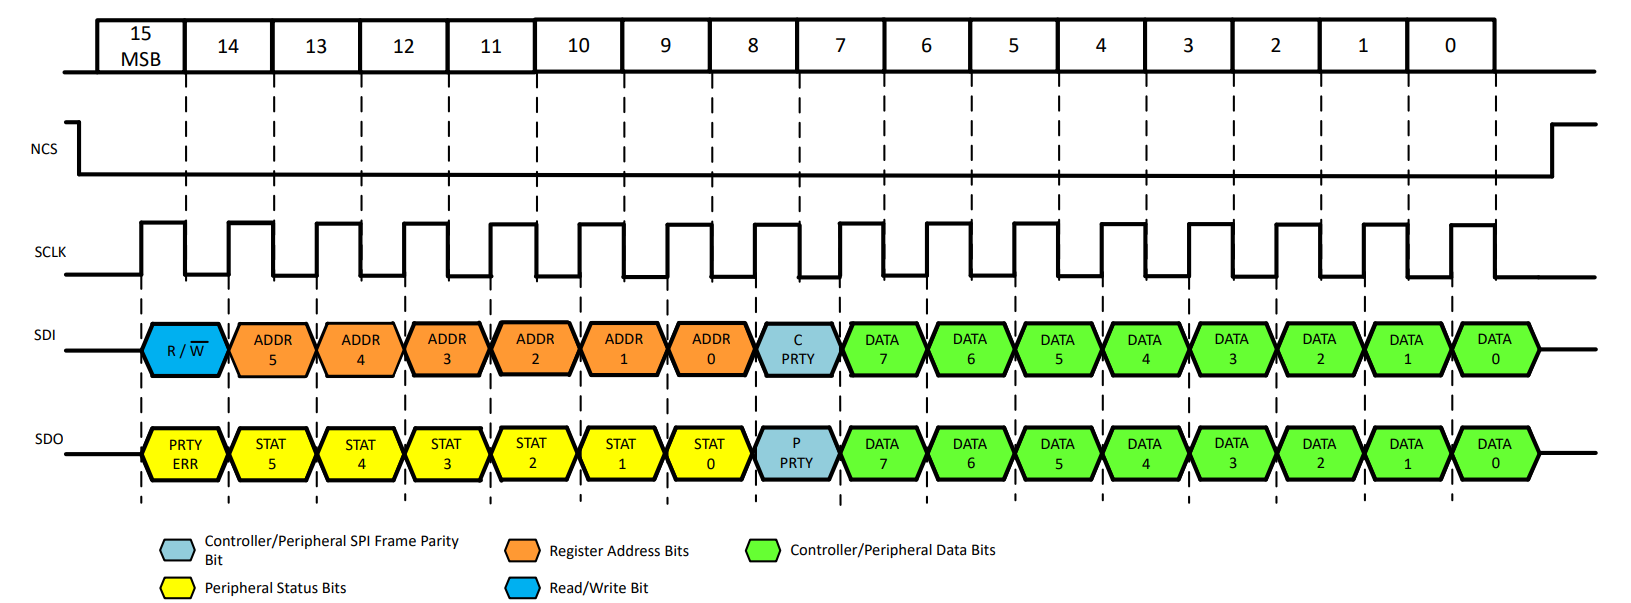
\includegraphics[width=10cm]{figure/SPI Frame.png}
        \songti\zihao{5}\caption{SPI数据结构图1}
        \label{SPI数据结构图1}
    \end{figure}
    MCU通过SDI引脚向驱动芯片发送配置数据,通过SDO引脚接收驱动芯片返回的数据。SDI发送数据的第15位为读写选择位,当其选择为write模式或者read模式时,数据收发数据的结构都有所不同,如图\ref{SPI数据结构图2}所示。
    \begin{figure}[H]
        \centering
        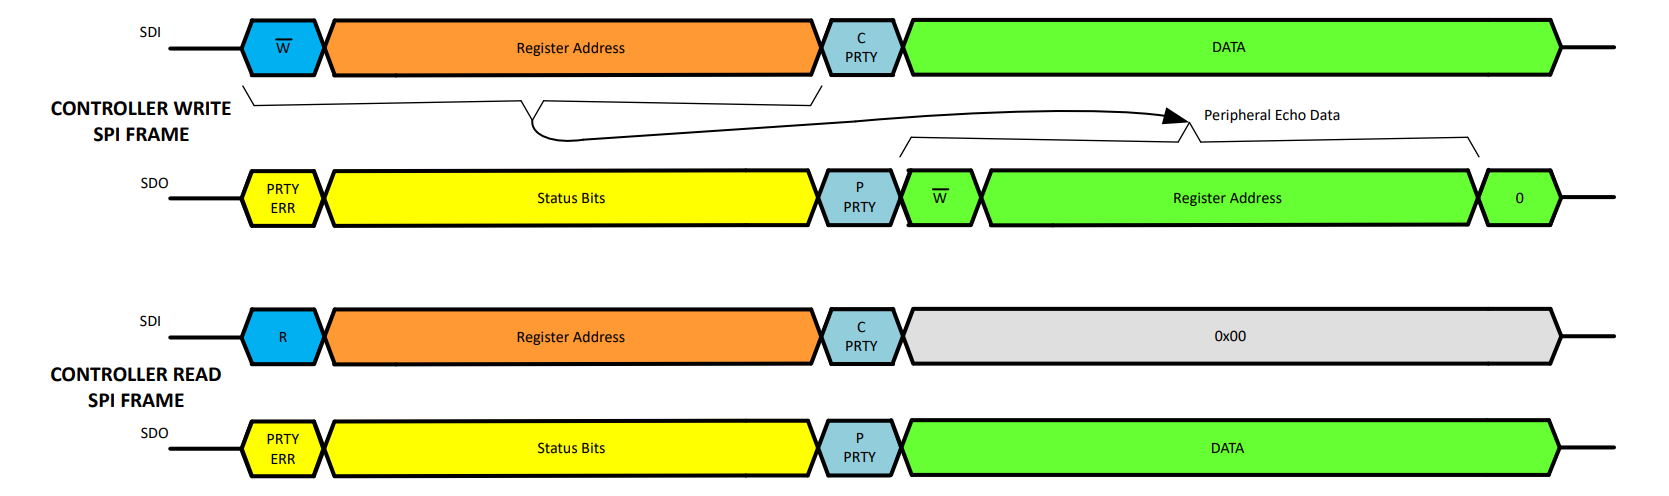
\includegraphics[width=12cm]{figure/SPI Transfer Sequence.png}
        \songti\zihao{5}\caption{SPI数据结构图2}
        \label{SPI数据结构图2}
    \end{figure}
    在write模式下,SDI14位-9位为寄存器地址,第8位为奇校验位,7位-0位为寄存器配置数据。SDO第一位为奇校验错误位,用于记录发送数据的奇校验是否通过,未通过校验时该位置1,14位-9位为驱动芯片的状态位,用于反映芯片当前的状态模式,如表\ref{芯片状态表}所示。第8位为奇校验位,7位-0位为写入寄存器的地址。\par
    
    \begin{table}[H]
        \centering
        \zihao{5}\caption{芯片状态表}
        \songti\zihao{5}
        \begin{tabular}{c|c}
            \hline
            \textbf{STATUS BIT }& \textbf{DESCRIPTION}      \\ \hline
            STAT 5 - VDRV\_READY    &   VDRV引脚达到配置电压值时置1  \\ \hline
            STAT 4 - PULSE\_NUM\_FLT &  发生脉冲数目错误是置1  \\\hline
            STAT 3 - DRV\_PULSE\_FLT &  脉冲发生无响应时置1 \\\hline
            STAT 2 - EE\_CRC\_FLT & 加载内部EEPROM存储器出现CRC错误时置1\\\hline
            STAT <1:0> - DEV\_STATE  &  \makecell{芯片模式:\\
                                        00 - 检测模式\\
                                        01 - 脉冲发生模式\\
                                        10 - 待机模式\\
                                        11 - 睡眠模式} \\\hline
            
      
            \end{tabular}
        \label{芯片状态表}    
         \end{table}
    在read模式下,SDI的14位-9位为读取寄存器地址,7位-0位为0,SDO的7位-0位为该寄存器内存储的数据。
    
    


    
    \noindent
    \textbf{6、寄存器配置}\par
    TUSS4470超声驱动芯片各寄存器的配置如表\ref{寄存器配置}所示。
      \begin{table}[H]
        \centering
        \zihao{5}\caption{寄存器配置}
        \songti\zihao{5}
        \begin{tabular}{c|c|c|c}
        \hline
        \textbf{寄存器名} & \textbf{缩写}& \textbf{地址} &\textbf{配置值}\\ \hline
        Bandpass filter settings&BPF\_CONFIG\_1&0x10& 0x25 \\ \hline
        Bandpass filter settings&BPF\_CONFIG\_2&0x11& 0x00\\ \hline
        Log-amp configuration&DEV\_CTRL\_1&0x12& 0xB3\\ \hline
        Log-amp configuration&DEV\_CTRL\_2&0x13& 0x02\\ \hline
        Log-amp configuration&DEV\_CTRL\_3&0x14& 0x03\\ \hline
        VDRV Regulator Control&VDRV\_CTRL&0x16& 0x07\\ \hline
        Echo Interrupt Control &ECHO\_INT\_CONFIG&0x17&0x0F \\ \hline  
        Zero Crossing configuration &ZC\_CONFIG&0x18& 0xD4\\ \hline 
        Burst pulse configuration &BURST\_PULSE&0x1A& 0x08\\ \hline 
        Time of Flight Config&TOF\_CONFIG&0x1B& 0x00\\ \hline 
        Fault status bits&DEV\_STAT&0x1C& 0x00\\ \hline
        Device ID&DEVICE\_ID&0x1D& 0x00\\ \hline
        Revision ID &REV\_ID&0x1E& 0x00\\ \hline
        
            \end{tabular}
        \label{寄存器配置}    
         \end{table}
    其中BPF\_CONFIG\_1用于配置带通滤波器的中心频率,该频率需匹配超声波传感器的工作频率,查阅芯片手册可以得知,当寄存器配置为0x25时,带通滤波器的中心频率为301.28KHZ,与超声波传感器最匹配;\par
    BPF\_CONFIG\_2用于设置滤波器的Q因素,修正滤波器的频率范围;\par
    DEV\_CTRL\_1用于调整对数放大器参数,通过查阅资料,将其设置为0xB3;\par
    DEV\_CTRL\_2用于设置放大器(LNA)的增益;\par
    DEV\_CTRL\_3用于配置脉冲发生的模式,本设计采用IO\_MODE3,故将该寄存器配置为0x03;\par
    VDRV\_CTRL寄存器主要用于配置VDRV引脚的参考电压,当该引脚的实际电压超过参考电压时,驱动芯片的VDRV\_READY状态位置1,然后通过SPI将该状态位返回至MCU芯片。本设计采用12V的驱动电压,根据芯片手册所给出的公式得出该寄存器配置为0x0F;\par
    ECHO\_INT\_CONFIG用于配置VOUT引脚的参考阈值,当VOUT引脚输出电压超过该阈值时,即判断为检测到物体,OUT4拉高。本设计所需的检测距离为200mm,根据实验将电压阈值设置为1V,寄存器配置为0x0F;\par
    ZC\_CONFIG寄存器用于配置过零信号,以提高传感器的抗干扰性。选取380mV作为零点,配合OUT4信号进行接近检测,寄存器配置为0xD4;\par
    BURST\_PULSE寄存器的前五位用于配置每个脉冲波的脉冲数,本设计的脉冲数为8,故配置其为0x08;\par
    TOF\_CONFIG寄存器用于待机模式和睡眠模式的设置,本设计只使用到脉冲发生模式和检测模式,暂不需要使用到这两种模式,故配置为0x00;\par
    DEV\_STAT寄存器为芯片的状态寄存器,包括了VDRV状态、脉冲发生状态,可供MCU芯片读取,故不需写入数据,配置为0x00;\par
    DEVICE\_ID和REV\_ID寄存器存放的是芯片的固定参数,无需写入,配置为0x00。
    
    \subsubsection{脉冲发生模块}
    TUSS4470超声驱动芯片有4种脉冲模式来为超声传感器提供激励。在每个模式中,超声发出脉冲的频率取决于外部输入时钟的频率,这可以让使用者产生精确的时钟来匹配超声波传感器的固有频率,从而产生最高的声压水平。在本设计中,将采用脉冲模式1来产生脉冲信号。\par
    在脉冲模式1中,IO2引脚将作为外部时钟输入引脚,IO1作为控制引脚。如图\ref{脉冲模式1}所示,当IO1引脚拉低时,进入脉冲发生模式,在检测到IO2引脚的第一个下降沿时,开始产生脉冲,产生脉冲的数目将通过下降沿的个数来计算。4当产生脉冲的数目达到寄存器内的配置值,或者IO1引脚的信号拉高时,都将退出脉冲发生模式,取决于哪个事件先发生。在进入到脉冲发生模式后,OUTA和OUTB引脚的信号都将取决于IO1和IO2引脚,当需要连续产生多次脉冲时,IO2引脚的信号需要经历低-高-低的过程。
     \begin{figure}[H]
        \centering
        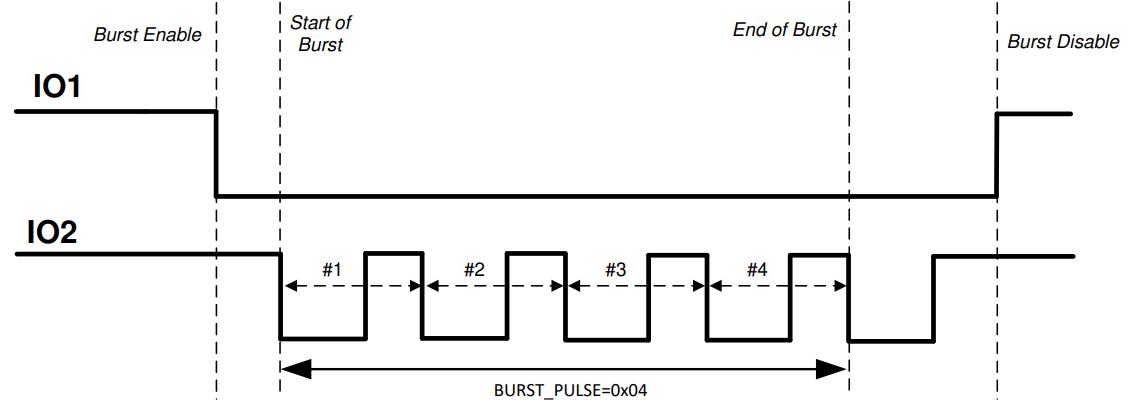
\includegraphics[width=12cm]{figure/IO MODE1.png}
        \songti\zihao{5}\caption{脉冲模式1}
        \label{脉冲模式1}
    \end{figure}
    在本设计的脉冲发生模块中,将能产生指定频率,指定脉冲数,指定次数的脉冲波,程序流程图如图所示。
    
   
    
    
    
       \begin{figure}[H]
        \centering
        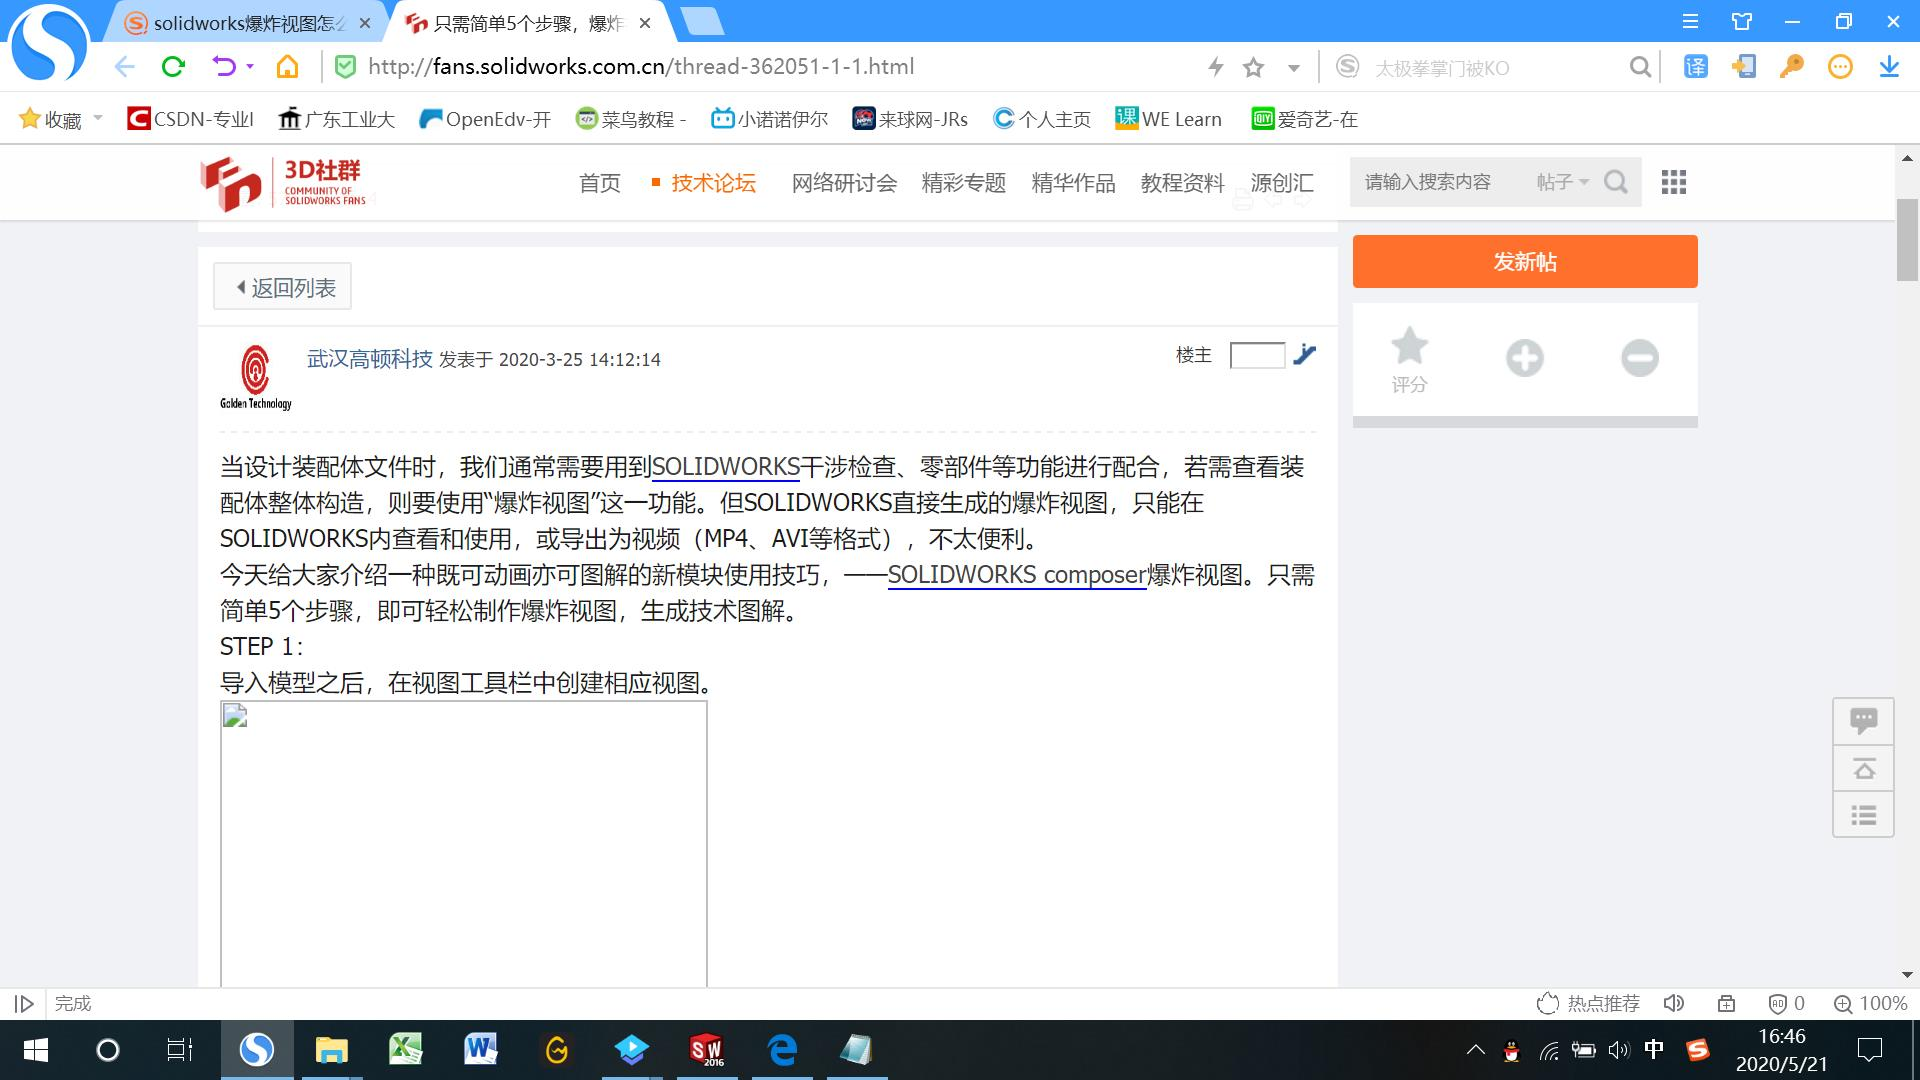
\includegraphics[width=12cm]{figure/1.jpg}
        \songti\zihao{5}\caption{脉冲发生模块程序流程图}
        \label{脉冲发生模块程序流程图}
    \end{figure}
    
  
    \subsubsection{检测计数模块}
    \songti\zihao{-4}{
    该模块功能在于,对到达指定位置的钢化玻璃进行计数,可以准确得知流水线上到位钢化玻璃的数量,便于后续统计。
    \begin{figure}[H]
        \centering
        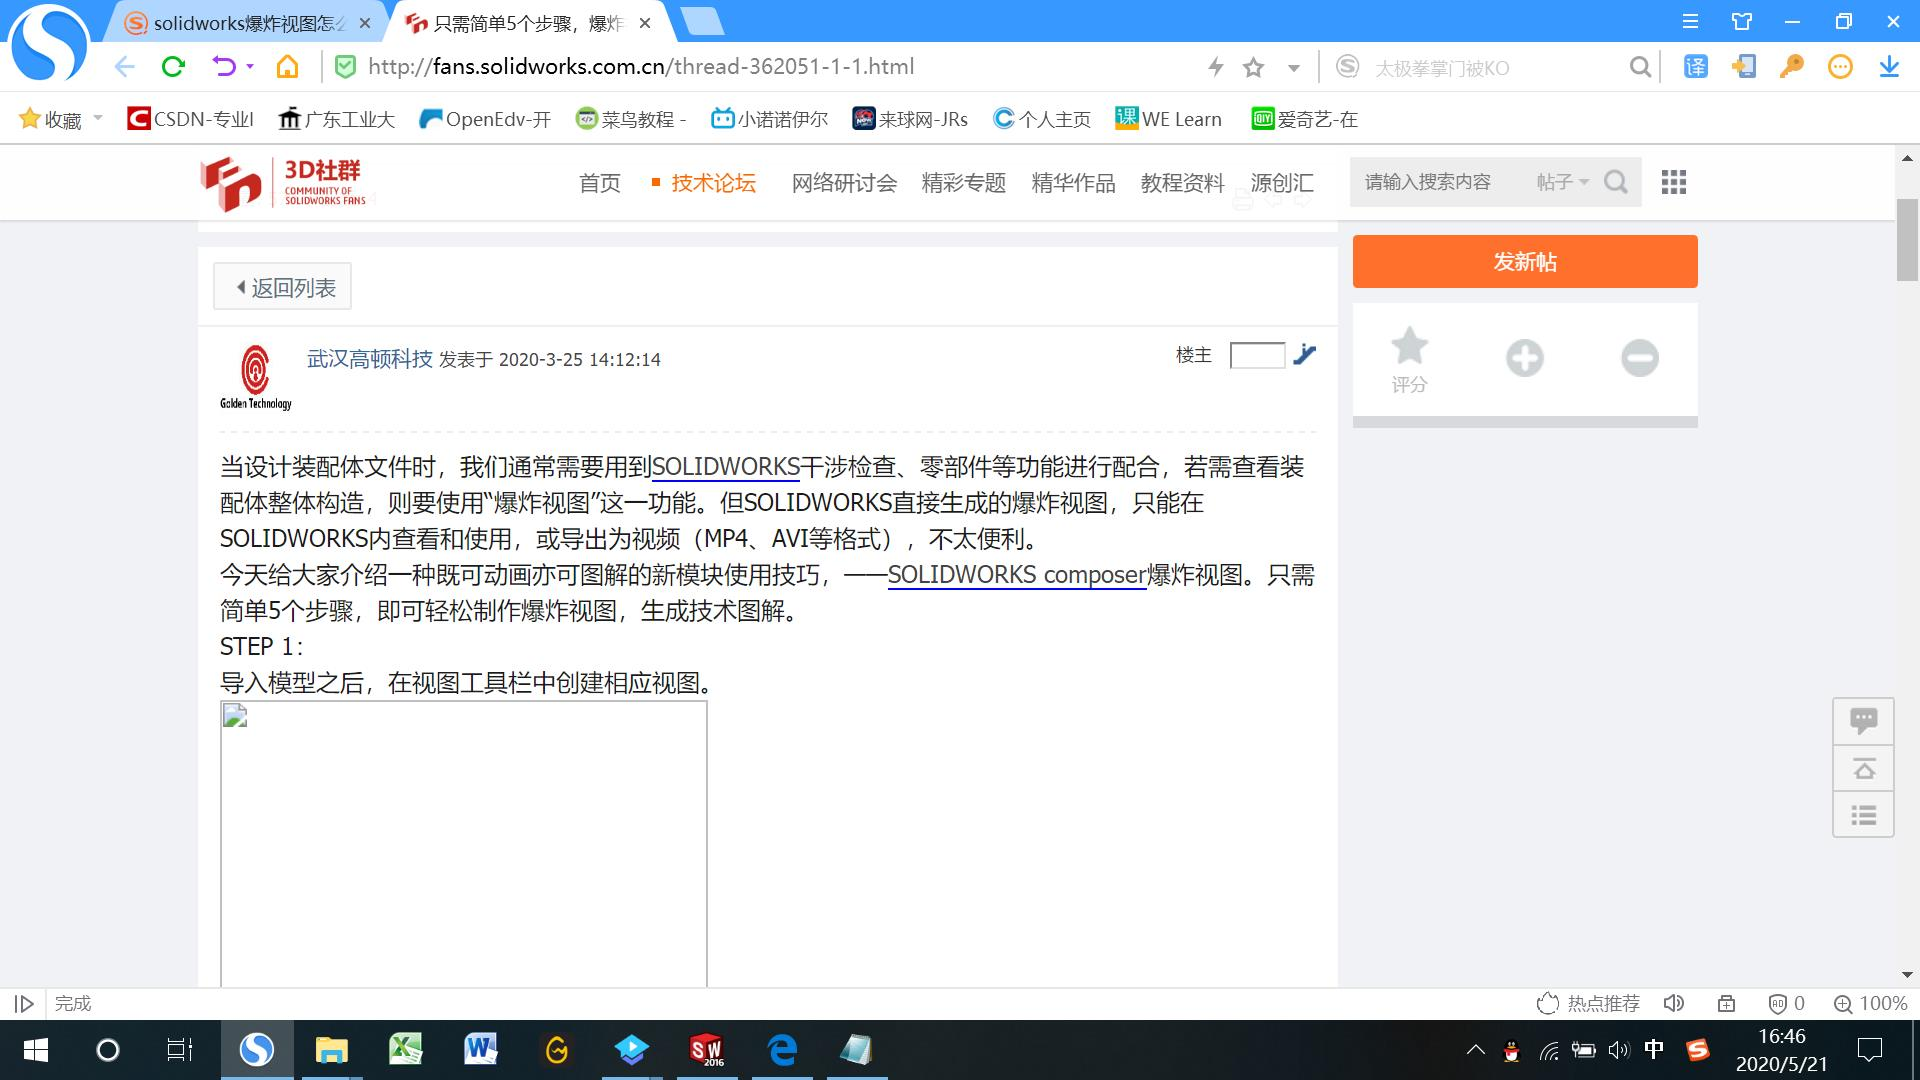
\includegraphics[width=10cm]{figure/1.jpg}
        \songti\zihao{5}{\caption{检测计数模块流程图}}
        \label{检测计数模块流程图}
    \end{figure}

    其功能实现流程如图\ref{检测计数模块流程图}示:当一块玻璃到位后,到位检测指示灯LED1变亮,CPLD芯片从CT\_1口得到一个高电平信号,计数寄存器object\_num加1;当钢化玻璃离开检测区域后,检测指示灯灭,等待下一块玻璃到位。\par
    
    }   
    
    \subsubsection{仿真模拟}
    
    %------------------第五章---------------------------
    \newpage
	\section{超声波接近传感器实物制作与检测}
 \subsection{超声波接近传感器实物制作}
 \subsubsection{超声波接近传感器焊接}
	在完成硬件部分和软件部分的设计之后,就将进行元器件采购、打板、实物焊接制作。如图\ref{PCB实物焊接图}为焊接完成后的实物图。
	\begin{figure}[!h]
	    \centering
	    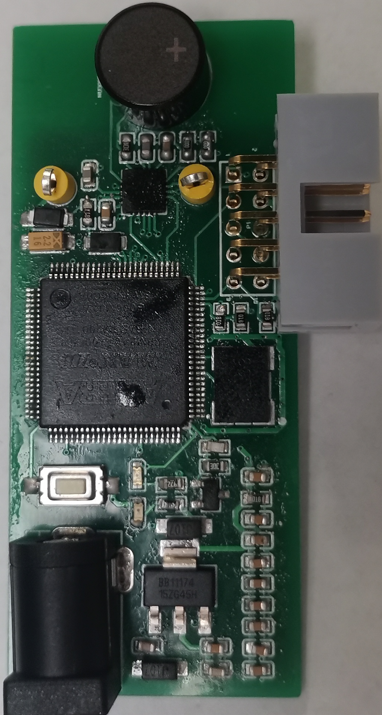
\includegraphics[width=8cm,angle=-90]{figure/physical map.png}
	    \caption{PCB实物焊接图}
	    \label{PCB实物焊接图}
	\end{figure}\par
 在焊接开始之前,为方便后续的焊接,首先要确定各个元器件的焊接顺序。根据焊接经验,本设计选取的焊接顺序为CPLD芯片->TUSS4470超声驱动芯片->其它贴片器。在确定好焊接顺序后,就可以开始正式焊接。首先清理电路板并检查电路板上是否有问题(例如:短路、断路等),然后用电烙铁焊接好CPLD芯片,并确保各引脚间没有存在虚焊、粘结等情况;焊接完成CPLD芯片后进行驱动芯片的焊接,首先在电路板上涂上焊锡膏,将芯片正确摆放,用热风枪加热焊锡膏使其融化,并轻轻按压芯片使焊盘上锡,最后再用电烙铁将粘结的引脚分离;其它的贴片器件贼按照涂焊锡膏、摆放器件、用热风枪加热的步骤来完成焊接;插件使用电烙铁来焊接。\par
 在完成焊接后,还需检查焊点是否光滑、平整、没有短路和冷焊等问题,使用显微镜或放大镜检查焊点的质量。检查无误后,再用洗板水清洗电路板,去除在焊接过程中多余的松香、锡膏等杂物。清洗完成后,就可以通电进行程序的调试。

\subsubsection{超声波接近传感器调试}
通过示波器对各引脚输出的波形进行检测,然后修改程序,直至每个引脚可以输出正常波形,以下为传感器正常工作时各引脚输出的波形。\par
	\begin{figure}[!h]
	    \centering
	    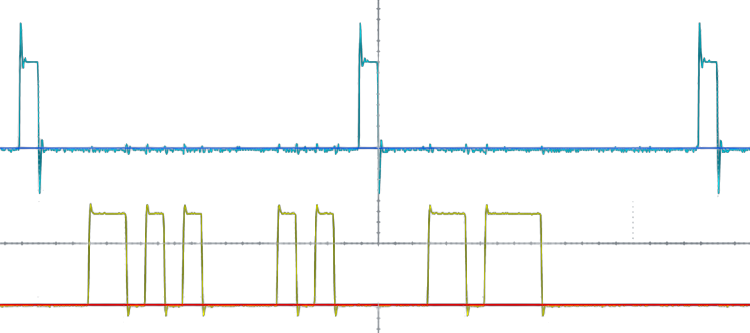
\includegraphics[width=8cm,height=3.5cm]{figure/debug waveform1.png}
	    \caption{SPI发送数据波形图}
	    \label{SPI发送数据波形图}
	\end{figure}\par
 如图\ref{SPI发送数据波形图},为采样率100$MHz$时示波器采集的波形,上方蓝色的为NSS端口的波形,下方黄色的为MOSI端口向驱动芯片发送的配置数据。可以看到,当NSS信号拉低时,MCU开始发送数据,等待一帧数据发送完成后,NSS拉高,并且在下一帧数据发送前,NSS会再次拉低,以实现低-高-低的过程。本设计的程序可以实现连续发送10帧配置数据的功能。
    \begin{figure}[!h]
	    \centering
	    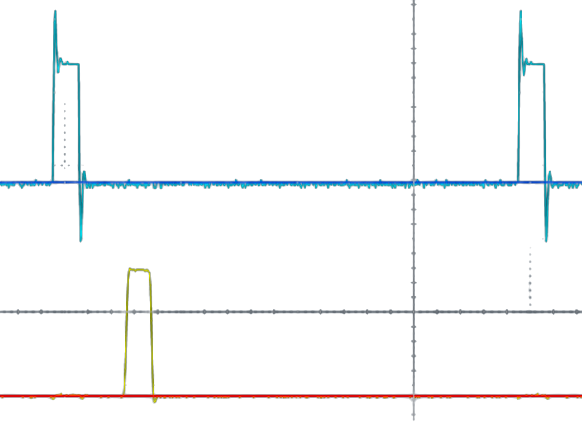
\includegraphics[width=8cm,height=3.5cm]{figure/debug waveform2.png}
	    \caption{SPI接收数据波形图}
	    \label{SPI接收数据波形图}
	\end{figure}\par
 图\ref{SPI接收数据波形图}为SPI接收数据的波形图,上方蓝色的波形为NSS端口发送的信号,下方黄色的为MISO端口接收的波形信号。当每次NSS信号拉低时,超声驱动芯片会向MCU返回数据,返回数据的结构如图\ref{SPI数据结构图1}和表\ref{芯片状态表}所示,当传感器正常工作时,只有VDRV\_READY状态位为1,其余位都为0。
 \newpage
   \begin{figure}[!h]
	    \centering
	    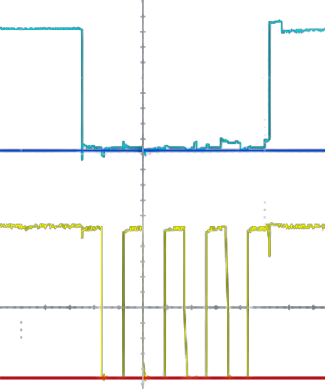
\includegraphics[width=8cm,height=3.5cm]{figure/debug waveform9.png}
	    \caption{io1、io2引脚波形图}
	    \label{io1、io2引脚波形图}
	\end{figure}\par
 如图\ref{io1、io2引脚波形图}所示,蓝色波形为io1引脚输出信号,黄色波形为io2引脚信号,两引脚按照IO模式3产生信号,当io1引脚信号拉低时,io2开始产生波形,直到产生指定脉冲数波形后,io1拉高,停止产生波形。
 
 \begin{figure}[!h]
	    \centering
	    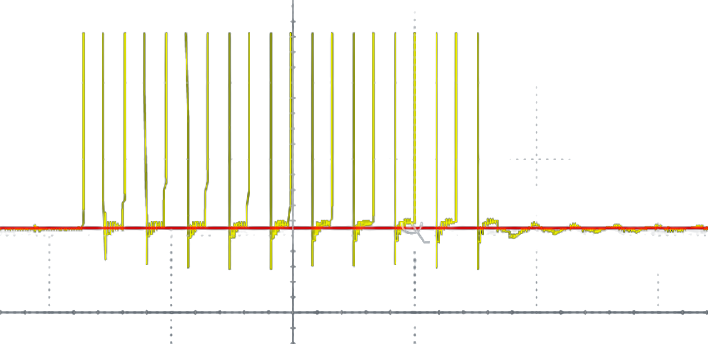
\includegraphics[width=8cm,height=3.5cm]{figure/debug waveform3.png}
	    \caption{超声探头波形图1}
	    \label{超声探头波形图1}
	\end{figure}\par
 图\ref{超声探头波形图1}为OUTA和OUTB引脚输出的波形,采样频率50$MHz$,可以看到,探头发出了10个周期频率为300$MHz$的脉冲波。
  \begin{figure}[!h]
	    \centering
	    \includegraphics[width=8cm]{figure/debug waveform4.png}
	    \caption{超声探头波形图2}
	    \label{超声探头波形图2}
	\end{figure}\par
 图\ref{超声探头波形图2}为示波器采样率10$MHz$时采集到的波形,超声探头连续的发送波形,以10个脉冲为发送周期,每过$2.4ms$完成一次脉冲的发送。
 \newpage
 \begin{figure}[!h]
	    \centering
	    \includegraphics[width=8cm,height=3.5cm]{figure/debug waveform5.png}
	    \caption{VOUT引脚波形图(无物体遮挡)}
	    \label{VOUT引脚波形图(无物体遮挡)}
	\end{figure}\par

 图\ref{VOUT引脚波形图(无物体遮挡)}为无物体遮挡的情况下,VOUT引脚输出的波形,采样频率为1$MHz$。第一个波峰为探头发出脉冲信号时所引起的干扰,在设计检测程序时需要屏蔽该段的信号,经测量,该段信号的持续时间约为发射脉冲后的$0.5ms$。
 \begin{figure}[!h]
	    \centering
	    \includegraphics[width=8cm,height=3.5cm]{figure/debug waveform6.png}
	    \caption{VOUT引脚波形图(有物体遮挡)}
	    \label{VOUT引脚波形图(有物体遮挡)}
	\end{figure}\par
 图\ref{VOUT引脚波形图(有物体遮挡)}为有物体遮挡时VOUT引脚的输出波形,采样频率为1$MHz$。当有物体遮挡时,发射的10个脉冲波遇到物体后会进行反射,重新被探头所接收。经过芯片的放大解调处理,形成第二个峰值较低的波峰。
 \begin{figure}[!h]
	    \centering
	    \includegraphics[width=8cm,height=3.5cm]{figure/debug waveform7.png}
	    \caption{OUT4引脚波形图(无物体遮挡)}
	    \label{OUT4引脚波形图(无物体遮挡)}
	\end{figure}\par
 图\ref{OUT4引脚波形图(无物体遮挡)}为OUT4引脚的输出波形,采样频率为1$MHz$。根据芯片手册中所介绍内容,我们不难知道,当VOUT引脚的电压值超过所设定的阈值时,OUT4引脚就会拉高。上图所示波形VOUT的阈值设置为0.9V,当VOUT形成第一个波峰时,电压值超过0.9V的频段OUT4也会拉高。
 \newpage
 \begin{figure}[!h]
	    \centering
	    \includegraphics[width=8cm,height=3.5cm]{figure/debug wave form8.png}
	    \caption{OUT4引脚波形图(有物体遮挡)}
	    \label{OUT4引脚波形图(有物体遮挡)}
	\end{figure}\par
 图\ref{OUT4引脚波形图(有物体遮挡)}为有物体遮挡时OUT4引脚输出的波形,采样频率为1$MHz$。当有物体遮挡时,VOUT处理回波产生第二个波峰,而这第二个波峰才是检测所需要用到的有效信号。在这个频段中,VOUT电压值超过所设定的阈值,OUT4第二次拉高,该信号将作为检测物体的重要触发事件。为屏蔽OUT4的第一次拉高信号,在MAIN模块中需要延时一段时间,跳过第一个信号后再开始进行检测,此时只会检测到OUT4的第二个拉高信号,检测有效。

 

\subsection{超声波接近传感器实验}

\subsubsection{实验器材}
在本设计的实验测试当中,采用新型的虚拟示波器,如图所示。该示波器是一种基于计算机的数字示波器,通过采集模拟信号并转换为数字信号,再利用计算机对信号进行处理、显示和分析,实现波形显示的功能。配合功能强大的上位机软件,该示波器具有显示灵活、精度高、波形数据可存储等优点,十分适合本设计的试验调试。\par
其它实验材料如图所示,包括了直尺、12V直流电源供电插头、$100mm\times100mm$的测试板材。

\subsubsection{超声波接近传感器性能参数测试}
在本设计的实验中,对传感器的各性能参数进行了测试,如表所示,有效检测范围为$100mm\sim200mm$,传感器精度为$1mm$,LED检测指示灯刷新的频率为$Hz$,即每过$10ms$完成一次检测状态的刷新。
 \begin{table}[!h]
        \centering
        \caption{性能参数表}

        \begin{GDUTtable}{\textwidth}{Y Y Y}
            \textbf{参数名 }& \textbf{参数值} &\textbf{单位}    \\ 
            \hline
            检测范围    &   100-200 & $mm$  \\ 
            检测精度 &  1 & $mm$  \\\
            检测周期 &  2.4 &$ms$  \\      
      
            \end{GDUTtable}
        \label{芯片状态表}    
         \end{table}


\subsubsection{超声波接近传感器稳定性测试}
在有干扰的情况下进行性能测试

干扰源选取:可度量的干扰源

在检测周期不变的情况下,调整检测逻辑,观察应对干扰的效果

\subsubsection{不同材料的测试}
将测试物体放置在距离超声波传感器$150mm$的位置,每次发射脉冲数为8的脉冲,对于不同材料的检测物体进行测试,观察VOUT波形的峰值,测量五次取平均值。实验材料为亚克力板、纸板、陶瓷板、玻璃,实验结果如表所示。
 \begin{table}[!h]
        \centering
        \caption{不同材料测试结果}
        \begin{GDUTtable}{\textwidth}{Y Y Y}
            \textbf{材料类型 }& \textbf{VOUT波形峰值} &\textbf{单位}      \\
            \hline
            亚克力板 & 0.79 &v  \\
            纸板 & 0.78 &v \\
            陶瓷板 & 0.79 &v\\
            玻璃 & 0.8 &v\\
            \end{GDUTtable}
        \label{芯片状态表}    
         \end{table}
根据实验结果,我们可以画出各材料对应回波峰值的折线图,如图所示。通过观察图形,我们可以得知,VOUT回波与物体的材质并无太大关系,当检测物体材质改变时,VOUT引脚输出的波形并没有太大的变化,而与反射脉冲波的强度有关。

\subsubsection{不同脉冲数的测试}
将检测物体放置在距离超声波传感器$150mm$的位置,改变每次发送脉冲波的脉冲数,观察VOUT波形峰值的变化情况。
亚克力板,脉冲数3,5,7,9,11
纸板
石板
石英玻璃,脉冲数3,5,7,9,11
图中每个数据点都为实验五次取平均值后的结果,可以看到,当每次发射脉冲波的脉冲数越多时,VOUT引脚的峰值就越大。



\subsubsection{不同距离的测试}
以亚克力板作为检测物体,将测试物体放置在距离传感器$50mm$,$100mm$,$150mm$,$200mm$,$250mm$的位置,测试其回波信号$t$值的大小,$t$值为波峰距离检测周期起点的时间,实验结果如图所示。


当检测距离增加时,VOUT第二个波峰的峰值在不断减小,距离检测起点的时间也在不断增加,与图\ref{VOUT输出}对比,实验结果相近,可以证明传感器脉冲发射检测没有异常。
\subsection{本章小结}
本章首先介绍了超声波接近传感器实物焊接的流程,然后列举了实物调试过程中所记录的波形图,将其与仿真波形进行了比较。然后介绍了实验器材以及五种实验方案的设计,列举了处理后的实验数据,并对实验结果进行初步分析。下一章将对本设计所存在的不足进行总结,提出对后续的展望。








\newpage
\section{总结与展望}
在本研究中,我们成功地基于TUSS4470芯片设计并制作了超声波接近传感器,并使用CPLD芯片实现了传感器的控制电路。我们详细地介绍了超声波传感器的工作原理和设计流程,并对CPLD芯片的控制电路、电源电路、JTAG下载模块和时钟模块等进行了详细的分析和讨论。通过实验验证,我们证明了该传感器具有高精度、高灵敏度、低功耗等优点,可应用于机器人导航、工业自动化、智能家居等领域。\par
尽管本设计完成了一定成果,但仍然存在一些局限性和不足之处。未来的研究可以从以下几个方面进行深入研究:\par
将CPLD芯片用价格低廉、封装小的国产FPGA芯片替代。随着国内FPGA技术的发展和成熟,其在性能、功耗和成本等方面的优势逐渐显现,通过使用国产FPGA芯片,可以进一步降低传感器成本,提高传感器的经济性。同时,在本设计中CPLD芯片的引脚并未被完全利用,存在浪费,可选择引脚更少的国产FPGA,提高引脚的利用率。此外,国产FPGA的封装只有CPLD芯片的$\frac{1}{4}$,可以极大减小超声传感器的尺寸,利于其在生产线上的布置。\par
改进硬件电路设计,本设计在进行实验的过程中,发现PCB电路板存在工作不稳定的情况,经过排查,发现降压芯片的选取不合理,功率不满足电路板的需求,导致电路板容易发热。后续需要优化电路板设计,优化器件选型,提高电路板的稳定性和可靠性。\par
改善PCB布局设计,减小信号间的相互干扰。在本设计的PCB布局中虽然已经考虑到了信号间的隔离,但是仍然存在干扰,后续需要继续优化PCB的设计,可将二层板替换成四层板,从而可以更好的将模拟信号、数字信号、电源信号布局分离,提高信号的稳定性。\par
改进超声波传感器的信号处理算法以及检测策略,进一步提高传感器的精度和灵敏度。在本设计中,一个检测周期进行了五次的检测,耗时10ms,而检测策略的选择则需要根据应用场景进行判断,这需要进行大量的实验才可以得出其规律,这都是未来可以进行的研究工作。\par
针对不同领域的应用场景,对传感器进行测试实验。在本设计中,只对于几种材料、距离进行测试实验,然而在实际的应用中,这几组实验是远远不够的,需要对更多类型的材料、距离进行实验测试。如若有需求,还应该搭建更加稳定的实验平台,对于测试物体的检测距离、移动速度都加以更精确的控制。\par
在未来的研究中,我们将进一步深入探究传感器技术的发展和应用,为实现智能化、自动化的社会和工业系统做出更多的贡献。


%!TEX root = ../main.tex
\makesection{结论}

%%!TEX root = ../main.tex
\section{Ⅰ级叶/盘转子错频方案的对比分析}
在叶轮机械领域,对一个实际的叶盘转子,错频是指由于单个叶片之间因几何上或结构上的不同而造成的其在固有频率上的差异\cite{刘国钧1979图书馆史研究}。
\subsection{多自由度系统的强迫响应分析}
由前面的分析可知,响应分析在数学上是一个具有 38 个自由度的二阶线性
微分方程的数值积分问题\cite{张和生1998地质力学系统理论, 1988汉语拼音正词法基本规则, 情感工学破解"舒服"之迷, 王明亮1998关于中国学术期刊标准化数据库系统工程的进展}。

\subsubsection{动态响应的计算方法}
\paragraph{系统的运动方程}
多自由度系统运动微分方程的一般形式为:……
\begin{enumerate}
    \item ……
    \item ……
\end{enumerate}

\paragraph{微分方程组的数值积分}
一介常系数微分方程组的初值问题可表述为:……

\subsubsection{强迫相应前的准备工作}
……


\begin{equation}
    \vec{P}_{i}(u)=\sum_{j=0}^{k} \vec{V}_{i} \Lambda_{i}\left(k ; \vec{\beta}_{1}, \cdots \vec{\beta}_{n} ; u\right)
\end{equation}

\begin{equation}
    \frac{|A(s)|^{2}}{|A(o)|^{2}}=\frac{\rho_{1} \rho_{2}}{\left(s+\rho_{1}\right)\left(s+\rho_{2}\right)}
\end{equation}

\begin{figure}[ht]
    \centering
    \includegraphics[width=0.5\textwidth]{example-image}\figurenotation{此图中的曲线对应关系与\autoref{fig:figname1}相同}
    \caption{部分相干调解与非相干解调平均误码性能的比较}
\end{figure}

\begin{figure}[ht]
    \centering
    \includegraphics[width=0.5\textwidth]{example-image}\figurenotation[]{
        1-太阳模拟器;2-单管及31 个PCM 容器;3-气泵;\\
        4-干燥过滤器;5-手动调节阀;6-孔板流量计;\\
        7-空气预热器;8,9-调功器;10-空气换热器.
    }
    \caption{单管换热系统流程图}
    \label{fig:figname1}
\end{figure}


\begin{figure}[ht]
    \subfloat[分布符合 $1/f$ 规律图]{\includegraphics[width = 0.3\textwidth]{example-image}}
	\hfill
	\subfloat[大小与色彩]{\includegraphics[width = 0.3\textwidth]{example-image}}
	\hfill
	\subfloat[间距、大小与色彩均符合 $1/f$ 规律图符合 $1/f$ 规律图]{\includegraphics[width = 0.3\textwidth]{example-image}} 
    \caption{图案例}    %大图名称
    \label{fig:figname2}    %图片引用标记
\end{figure}
    
引用图片样例如下:
\begin{itemize}
    \item 只引用编号:\verb|\ref{fig:figname1}| \ref{fig:figname1}
    \item 引用类型和编号:\verb|\autoref{fig:figname1}| \autoref{fig:figname1}
    \item 引用类型、编号、标题:\verb|\fullref{fig:figname1}| \fullref{fig:figname1}
\end{itemize}


\begin{table}[ht]
    \caption{方法——干扰抑制结果}
    \label{tab:1}
    \centering
    \begin{GDUTtable}{\textwidth}{Y|Y|Y|Y|Y}
        干扰类型                   & 目标信号                 & 阵元数                & 干扰采样值数 & SINR(dB) \\ \hline
        \multirow{4}{*}{第一类干扰} & \multirow{2}{*}{信号1} & 8                  & --     & 30.58    \\ \cline{3-5} 
                               &                      & 4                  & --     & 21.16    \\ \cline{2-5} 
                               & \multirow{2}{*}{信号4} & 8                  & --     & 38.28    \\ \cline{3-5} 
                               &                      & 4                  & --     & 19.41    \\ \hline
        \multirow{3}{*}{第二类干扰} & \multirow{3}{*}{信号4} & \multirow{2}{*}{8} & 30     & 4.69     \\ \cline{4-5} 
                               &                      &                    & 19     & 4.83     \\ \cline{3-5} 
                               &                      & 4                  & 30     & -0.42  \\
    \end{GDUTtable}
\end{table}



\begin{table}[ht]
    \caption{各组分$lgB_i$值}
    \label{tab:2}
    \centering
    \begin{GDUTtable}{\textwidth}{YYYYY}
        \multicolumn{1}{c|}{\multirow{4}{*}{序号}} & \multicolumn{2}{c|}{\multirow{2}{*}{$T = 1500K$}} & \multicolumn{2}{c}{\multirow{2}{*}{$T = 2000K$}} \\
\multicolumn{1}{c|}{}                    & \multicolumn{2}{c|}{}                             & \multicolumn{2}{c}{}                             \\ \cline{2-5} 
\multicolumn{1}{c|}{}                    & \multicolumn{2}{c|}{\multirow{2}{*}{组分$lgB_i$}}   & \multicolumn{2}{c}{\multirow{2}{*}{组分$lgB_i$}}   \\
\multicolumn{1}{c|}{}                    & \multicolumn{2}{c|}{}                             & \multicolumn{2}{c}{}                             \\ \hline
1                                        & abc                     & 123                     & abc                     & 123                    \\
2                                        & abc                     & 124                     & abc                     & 124                    \\
3                                        & abc                     & 125                     & abc                     & 125                    \\
4                                        & abc                     & 126                     & abc                     & 126                    \\
5                                        & abc                     & 127                     & abc                     & 127                    \\
6                                        & abc                     & 128                     & abc                     & 128                    \\
7                                        & abc                     & 129                     & abc                     & 129                    \\
8                                        & abc                     & 130                     & abc                     & 130                    \\
9                                        & abc                     & 131                     & abc                     & 131                    \\
10                                       & abc                     & 132                     & abc                     & 132                    \\
11                                       & abc                     & 133                     & abc                     & 133                    \\
12                                       & abc                     & 134                     & abc                     & 134                    \\
13                                       & abc                     & 135                     & abc                     & 135                    \\
14                                       & abc                     & 136                     & abc                     & 136                    \\
15                                       & abc                     & 137                     & abc                     & 137                   \\
    \end{GDUTtable}\tablenotation{“+”表示重要组分,“*”表示冗余组分.}
\end{table}

\begin{table}[ht]
    \caption{压降损失计算结果Pa}
    \label{tab:3}
    \centering
    \begin{GDUTtable}{\textwidth}{YYY}
        换热器 & 热边压降损失  & 冷边压降损失  \\ \hline
        初级  & 2974.37 & 2931.52 \\
        次级  & 2924.65 & 3789.76 \\
    \end{GDUTtable}
\end{table}


\makereference{Reference}


%!TEX root = ../main.tex
\makesection{致谢}
在广东工业大学本科四年的生活即将结束,回首过去四年,没有太多的风花雪月,有的是一个个踏实学习的日日夜夜。衷心感谢在这四年中给我提供帮助的人们。\par
首先我要感谢在大一大二指导过我画法几何的莫春柳老师,老师严谨的教学态度、幽默风趣的教学风格使我印象深刻。在老师指导我的过程中,老师不仅提供了教学上的帮助,还激发了我对本专业知识的浓厚兴趣,为我之后的学习生活提供了动力。\par
感谢机电工程学院仿生与智能机器人实验室的张涛老师,张老师专心科研、认真指导学生,在我大三参与实验室课题期间,每周都会组织组会进行汇报和指导工作。而更让我受益匪浅的是老师对待科研工作的巨大热情,感染着身边的人们,为我心中埋下了科研梦想的种子。\par
感谢我的毕业论文指导老师刘桂贤老师,老师对我们的毕业课题十分认真负责,在老师的指导和督促下,我们按时完成了要求的任务。\par
感谢在人生节点上给我提供建议和帮助的师兄师姐们,他们在我四年的生活中给予了我许多宝贵的意见。\par
感谢我的本科宿舍的室友们,四年里我们互相勉励,互相指导学习,完成了很多科目的课程设计、参加一次又一次科技学术比赛。来到毕业期每个人又各自找到了新的生活目标,去往五湖四海,有望江湖再见。
感谢我的家人对我的支持,在四年里不断对我进行支持和鼓励,为我的求学生涯提供了坚实的物质基础。\par
感谢机电工程学院足球队的队员们,在我心情烦闷时都会陪伴着我,为我提供建议、排忧解难。\par
感谢母校的培养,广东工业大学为我提供了学习的平台,无论今后身在何处,我都会秉持与发扬广工精神,以团结、勤奋、求是、创新的校训作为自己的行事准则,展现广工人“好用、实用、耐用、听话、出活”的人才气质。\par
最后,感谢本论文的评审老师以及参加答辩的专家、老师们,感谢你们对本论文提出的宝贵意见。

%!TEX root = ../main.tex
\makeappendix{主要程序代码}
\noindent
顶层模块
\lstinputlisting[language=Verilog]{./code/ultrasonic_sensor3_1.v}
\noindent
MAIN模块
\lstinputlisting[language=Verilog]{./code/main.v}
\noindent
SPI模块
\lstinputlisting[language=Verilog]{./code/spi.v}
\noindent
脉冲信号发生模块
\lstinputlisting[language=Verilog]{./code/pulse_generation.v}
\noindent
检测计数模块
\lstinputlisting[language=Verilog]{./code/detected_count.v}
TESTBENCH仿真激励文件
\lstinputlisting[language=Verilog]{./code/ultrasonic_sensor3_1.vt}

%!TEX root = ../main.tex
\makeappendix{器件采购表}

@booklet{ID,
	ALTauthor = {author},
	ALTeditor = {editor},
	title = {title},
	date = {date},
	OPTsubtitle = {subtitle},
	OPTtitleaddon = {titleaddon},
	OPTlanguage = {language},
	OPThowpublished = {howpublished},
	OPTtype = {type},
	OPTnote = {note},
	OPTlocation = {location},
	OPTchapter = {chapter},
	OPTpages = {pages},
	OPTpagetotal = {pagetotal},
	OPTaddendum = {addendum},
	OPTpubstate = {pubstate},
	OPTdoi = {doi},
	OPTeprint = {eprint},
	OPTeprintclass = {eprintclass},
	OPTeprinttype = {eprinttype},
	OPTurl = {url},
	OPTurldate = {urldate},
}


\end{document}